\documentclass[10pt]{article}
\usepackage[margin=2.2cm]{geometry}
\usepackage{booktabs,longtable,graphicx,array}
\usepackage[hidelinks]{hyperref}
\setlength{\tabcolsep}{4pt}
\newcommand{\stackcell}[1]{\begin{tabular}[t]{@{}l@{}}#1\end{tabular}}
\title{tropical: FloydWarshall}
\date{2026-10-24T16:14:17}
\begin{document}
\maketitle

\section{Key results}
This report covers 240 runs (5 seeds; 0 diverged) under frozen hash \texttt{765d817c3d73}.
\paragraph{Where to look.} The headline metric is \texttt{ood\_len\_f1} (higher is better).
\autoref{fig:ood_len_f1} plots it against \texttt{fishr\_lambda}.
\autoref{tab:summary-ood_len_f1} gives every cell's mean with its 95\% bootstrap CI.
\autoref{tab:control-ood_len_f1} compares each level with the control.
\autoref{tab:trend-ood_len_f1} gives the trend.
\autoref{tab:paired-ood_len_f1} gives the paired contrasts.
Its tests take the parametric path: values away from the metric bounds.
Cells are compared within a seed: a seed index fixes the data and the initialization.
Comparisons are marked significant at $p < 0.05$ after the stated correction.

\subsection{\texttt{ood\_len\_f1}}
\begin{figure}[tbp]
\centering
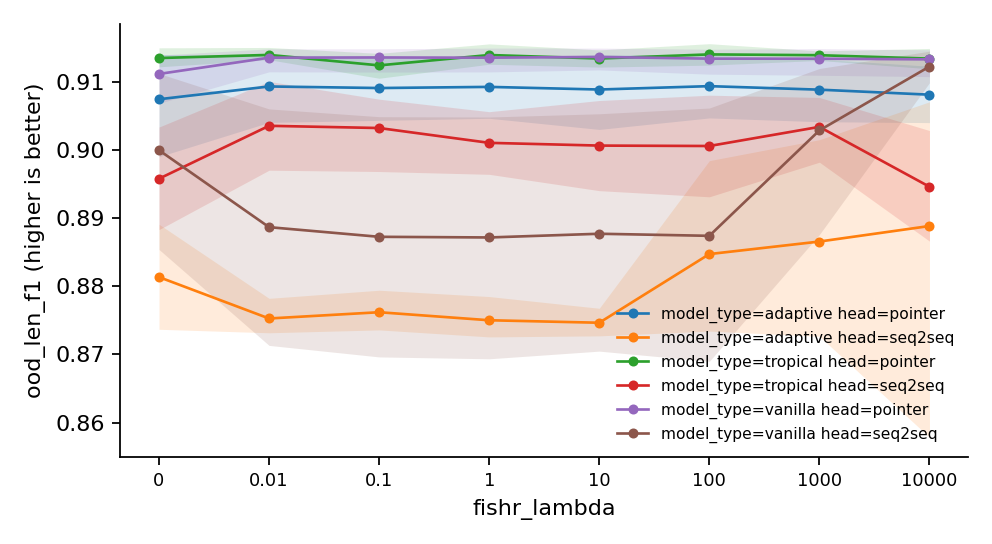
\includegraphics[width=\textwidth]{metric_ood_len_f1.png}
\caption{\texttt{ood\_len\_f1} against \texttt{fishr\_lambda}: the mean over seeds with a 95\% bootstrap CI, one line per combination of the other factors.}
\label{fig:ood_len_f1}
\end{figure}

{\small
\begin{longtable}{lllrlrrr}
\caption{\texttt{ood\_len\_f1} per cell: mean, 95\% bootstrap CI, SD, seeds, diverged runs.}\label{tab:summary-ood_len_f1}\\
\toprule
\texttt{model\_type} & \texttt{head} & \texttt{fishr\_lambda} & mean & 95\% CI & SD & $n$ & div.\\
\midrule
\endhead
adaptive & pointer & 0 & 0.9074 & [0.899, 0.914] & 0.0097 & 5 & 0\\
adaptive & pointer & 0.01 & 0.9093 & [0.904, 0.914] & 0.00625 & 5 & 0\\
adaptive & pointer & 0.1 & 0.9091 & [0.904, 0.914] & 0.0063 & 5 & 0\\
adaptive & pointer & 1 & 0.9092 & [0.905, 0.913] & 0.00574 & 5 & 0\\
adaptive & pointer & 10 & 0.9088 & [0.903, 0.914] & 0.00692 & 5 & 0\\
adaptive & pointer & 100 & 0.9093 & [0.905, 0.914] & 0.00609 & 5 & 0\\
adaptive & pointer & 1000 & 0.9088 & [0.904, 0.913] & 0.00594 & 5 & 0\\
adaptive & pointer & 1e+04 & 0.9081 & [0.904, 0.912] & 0.00533 & 5 & 0\\
adaptive & seq2seq & 0 & 0.8813 & [0.874, 0.889] & 0.00973 & 5 & 0\\
adaptive & seq2seq & 0.01 & 0.8753 & [0.873, 0.878] & 0.00333 & 5 & 0\\
adaptive & seq2seq & 0.1 & 0.8762 & [0.874, 0.879] & 0.00379 & 5 & 0\\
adaptive & seq2seq & 1 & 0.875 & [0.873, 0.878] & 0.00396 & 5 & 0\\
adaptive & seq2seq & 10 & 0.8746 & [0.873, 0.877] & 0.00292 & 5 & 0\\
adaptive & seq2seq & 100 & 0.8847 & [0.873, 0.898] & 0.0159 & 5 & 0\\
adaptive & seq2seq & 1000 & 0.8866 & [0.873, 0.901] & 0.0185 & 5 & 0\\
adaptive & seq2seq & 1e+04 & 0.8888 & [0.858, 0.907] & 0.0354 & 5 & 0\\
tropical & pointer & 0 & 0.9135 & [0.912, 0.915] & 0.00176 & 5 & 0\\
tropical & pointer & 0.01 & 0.9139 & [0.913, 0.915] & 0.00119 & 5 & 0\\
tropical & pointer & 0.1 & 0.9124 & [0.91, 0.914] & 0.00241 & 5 & 0\\
tropical & pointer & 1 & 0.9139 & [0.913, 0.916] & 0.00188 & 5 & 0\\
tropical & pointer & 10 & 0.9134 & [0.912, 0.915] & 0.00162 & 5 & 0\\
tropical & pointer & 100 & 0.914 & [0.912, 0.916] & 0.00197 & 5 & 0\\
tropical & pointer & 1000 & 0.9139 & [0.913, 0.915] & $8.98\times10^{-4}$ & 5 & 0\\
tropical & pointer & 1e+04 & 0.9134 & [0.912, 0.915] & 0.00195 & 5 & 0\\
tropical & seq2seq & 0 & 0.8958 & [0.888, 0.903] & 0.01 & 5 & 0\\
tropical & seq2seq & 0.01 & 0.9035 & [0.897, 0.91] & 0.00839 & 5 & 0\\
tropical & seq2seq & 0.1 & 0.9032 & [0.897, 0.907] & 0.00699 & 5 & 0\\
tropical & seq2seq & 1 & 0.901 & [0.896, 0.906] & 0.00612 & 5 & 0\\
tropical & seq2seq & 10 & 0.9006 & [0.894, 0.907] & 0.00855 & 5 & 0\\
tropical & seq2seq & 100 & 0.9006 & [0.893, 0.908] & 0.00993 & 5 & 0\\
tropical & seq2seq & 1000 & 0.9034 & [0.898, 0.908] & 0.00624 & 5 & 0\\
tropical & seq2seq & 1e+04 & 0.8946 & [0.887, 0.903] & 0.0104 & 5 & 0\\
vanilla & pointer & 0 & 0.9111 & [0.907, 0.914] & 0.00489 & 5 & 0\\
vanilla & pointer & 0.01 & 0.9135 & [0.911, 0.915] & 0.00236 & 5 & 0\\
vanilla & pointer & 0.1 & 0.9135 & [0.911, 0.915] & 0.00241 & 5 & 0\\
vanilla & pointer & 1 & 0.9135 & [0.911, 0.915] & 0.00236 & 5 & 0\\
vanilla & pointer & 10 & 0.9136 & [0.912, 0.915] & 0.00219 & 5 & 0\\
vanilla & pointer & 100 & 0.9134 & [0.911, 0.915] & 0.00254 & 5 & 0\\
vanilla & pointer & 1000 & 0.9134 & [0.911, 0.915] & 0.00271 & 5 & 0\\
vanilla & pointer & 1e+04 & 0.9133 & [0.911, 0.915] & 0.00284 & 5 & 0\\
vanilla & seq2seq & 0 & 0.8999 & [0.885, 0.911] & 0.0166 & 5 & 0\\
vanilla & seq2seq & 0.01 & 0.8887 & [0.871, 0.906] & 0.0229 & 5 & 0\\
vanilla & seq2seq & 0.1 & 0.8872 & [0.87, 0.905] & 0.0234 & 5 & 0\\
vanilla & seq2seq & 1 & 0.8872 & [0.869, 0.905] & 0.0236 & 5 & 0\\
vanilla & seq2seq & 10 & 0.8877 & [0.87, 0.905] & 0.0234 & 5 & 0\\
vanilla & seq2seq & 100 & 0.8874 & [0.869, 0.906] & 0.0249 & 5 & 0\\
vanilla & seq2seq & 1000 & 0.9029 & [0.888, 0.912] & 0.0168 & 5 & 0\\
vanilla & seq2seq & 1e+04 & 0.9122 & [0.91, 0.914] & 0.00296 & 5 & 0\\
\bottomrule
\end{longtable}
}

{\small
\begin{longtable}{lllrrrl}
\caption{\texttt{ood\_len\_f1}: each level of \texttt{fishr\_lambda} against its control (0), within each combination of the other factors. parametric: Dunnett vs control.}\label{tab:control-ood_len_f1}\\
\toprule
\texttt{model\_type} & \texttt{head} & \texttt{fishr\_lambda} & difference & 95\% CI & $p$ & \\
\midrule
\endhead
adaptive & pointer & 0.01 & 0.001874 & [-0.00975, 0.0135] & 0.9977 & \\
adaptive & pointer & 0.1 & 0.001644 & [-0.00998, 0.0133] & 0.9990 & \\
adaptive & pointer & 1 & 0.001812 & [-0.00982, 0.0134] & 0.9981 & \\
adaptive & pointer & 10 & 0.001426 & [-0.0102, 0.0131] & 0.9996 & \\
adaptive & pointer & 100 & 0.001921 & [-0.00971, 0.0135] & 0.9973 & \\
adaptive & pointer & 1000 & 0.001405 & [-0.0102, 0.013] & 0.9996 & \\
adaptive & pointer & 1e+04 & $6.698\times10^{-4}$ & [-0.011, 0.0123] & 1.0000 & \\
adaptive & seq2seq & 0.01 & -0.006069 & [-0.0336, 0.0215] & 0.9859 & \\
adaptive & seq2seq & 0.1 & -0.005151 & [-0.0327, 0.0224] & 0.9944 & \\
adaptive & seq2seq & 1 & -0.006328 & [-0.0339, 0.0212] & 0.9823 & \\
adaptive & seq2seq & 10 & -0.006693 & [-0.0343, 0.0209] & 0.9762 & \\
adaptive & seq2seq & 100 & 0.003377 & [-0.0242, 0.031] & 0.9996 & \\
adaptive & seq2seq & 1000 & 0.005214 & [-0.0224, 0.0328] & 0.9940 & \\
adaptive & seq2seq & 1e+04 & 0.007491 & [-0.0201, 0.0351] & 0.9581 & \\
tropical & pointer & 0.01 & $4.576\times10^{-4}$ & [-0.00263, 0.00355] & 0.9986 & \\
tropical & pointer & 0.1 & -0.001078 & [-0.00417, 0.00201] & 0.8738 & \\
tropical & pointer & 1 & $4.429\times10^{-4}$ & [-0.00265, 0.00353] & 0.9989 & \\
tropical & pointer & 10 & $-7.008\times10^{-5}$ & [-0.00316, 0.00302] & 1.0000 & \\
tropical & pointer & 100 & $5.329\times10^{-4}$ & [-0.00256, 0.00362] & 0.9965 & \\
tropical & pointer & 1000 & $4.158\times10^{-4}$ & [-0.00267, 0.0035] & 0.9992 & \\
tropical & pointer & 1e+04 & $-8.520\times10^{-5}$ & [-0.00317, 0.003] & 1.0000 & \\
tropical & seq2seq & 0.01 & 0.007759 & [-0.00707, 0.0226] & 0.5562 & \\
tropical & seq2seq & 0.1 & 0.007434 & [-0.0074, 0.0223] & 0.5988 & \\
tropical & seq2seq & 1 & 0.00526 & [-0.00957, 0.0201] & 0.8655 & \\
tropical & seq2seq & 10 & 0.004858 & [-0.00997, 0.0197] & 0.9023 & \\
tropical & seq2seq & 100 & 0.004797 & [-0.01, 0.0196] & 0.9073 & \\
tropical & seq2seq & 1000 & 0.007602 & [-0.00723, 0.0224] & 0.5766 & \\
tropical & seq2seq & 1e+04 & -0.001179 & [-0.016, 0.0137] & 1.0000 & \\
vanilla & pointer & 0.01 & 0.002386 & [-0.00269, 0.00746] & 0.6593 & \\
vanilla & pointer & 0.1 & 0.002413 & [-0.00266, 0.00749] & 0.6490 & \\
vanilla & pointer & 1 & 0.002382 & [-0.00269, 0.00745] & 0.6609 & \\
vanilla & pointer & 10 & 0.002494 & [-0.00258, 0.00757] & 0.6174 & \\
vanilla & pointer & 100 & 0.002241 & [-0.00283, 0.00731] & 0.7147 & \\
vanilla & pointer & 1000 & 0.002235 & [-0.00284, 0.00731] & 0.7170 & \\
vanilla & pointer & 1e+04 & 0.002138 & [-0.00293, 0.00721] & 0.7533 & \\
vanilla & seq2seq & 0.01 & -0.01129 & [-0.0471, 0.0245] & 0.9172 & \\
vanilla & seq2seq & 0.1 & -0.0127 & [-0.0485, 0.0231] & 0.8657 & \\
vanilla & seq2seq & 1 & -0.0128 & [-0.0486, 0.023] & 0.8617 & \\
vanilla & seq2seq & 10 & -0.01225 & [-0.0481, 0.0236] & 0.8834 & \\
vanilla & seq2seq & 100 & -0.01256 & [-0.0484, 0.0233] & 0.8715 & \\
vanilla & seq2seq & 1000 & 0.002902 & [-0.0329, 0.0387] & 1.0000 & \\
vanilla & seq2seq & 1e+04 & 0.01227 & [-0.0236, 0.0481] & 0.8829 & \\
\bottomrule
\end{longtable}
}

{\small
\begin{longtable}{llrrrrr}
\caption{\texttt{ood\_len\_f1} against log10 \texttt{fishr\_lambda}: parametric: OLS slope t-test, seed-bootstrap CI, with the Jonckheere--Terpstra ordered-trend $\tau$ and $p$.}\label{tab:trend-ood_len_f1}\\
\toprule
\texttt{model\_type} & \texttt{head} & estimate & 95\% CI & $p$ & JT $\tau$ & JT $p$\\
\midrule
\endhead
adaptive & pointer & $-1.422\times10^{-4}$ & [$-4.55\times10^{-4}$, $6.48\times10^{-5}$] & 0.7668 & -0.059 & 0.6717\\
adaptive & seq2seq & 0.00254 & [$5.02\times10^{-4}$, 0.00396] & 0.0601 & 0.147 & 0.2823\\
tropical & pointer & $5.173\times10^{-5}$ & [$-6.31\times10^{-5}$, $1.74\times10^{-4}$] & 0.7235 & 0.04 & 0.7688\\
tropical & seq2seq & $-9.620\times10^{-4}$ & [-0.00173, $-1.96\times10^{-4}$] & 0.1598 & -0.181 & 0.1776\\
vanilla & pointer & $-4.433\times10^{-5}$ & [$-1.24\times10^{-4}$, $1.22\times10^{-5}$] & 0.8210 & -0.0476 & 0.7297\\
vanilla & seq2seq & 0.003647 & [$5.46\times10^{-4}$, 0.00675] & 0.0408 & 0.173 & 0.1984\\
\bottomrule
\end{longtable}
}

{\small
\begin{longtable}{lrrrl}
\caption{\texttt{ood\_len\_f1}: paired contrasts by seed, Holm-corrected across the cells. parametric: paired t-test by seed, Holm.}\label{tab:paired-ood_len_f1}\\
\toprule
contrast (within) & difference & 95\% CI & $p$ & \\
\midrule
\endhead
\stackcell{model\_type: tropical - vanilla\\\footnotesize head=pointer fishr\_lambda=0 } & 0.002332 & [-0.00348, 0.00815] & 1.0000 & \\
\stackcell{model\_type: tropical - vanilla\\\footnotesize head=pointer fishr\_lambda=0.01 } & $4.037\times10^{-4}$ & [-0.00277, 0.00358] & 1.0000 & \\
\stackcell{model\_type: tropical - vanilla\\\footnotesize head=pointer fishr\_lambda=0.1 } & -0.001159 & [-0.00521, 0.00289] & 1.0000 & \\
\stackcell{model\_type: tropical - vanilla\\\footnotesize head=pointer fishr\_lambda=1 } & $3.929\times10^{-4}$ & [-0.00334, 0.00413] & 1.0000 & \\
\stackcell{model\_type: tropical - vanilla\\\footnotesize head=pointer fishr\_lambda=10 } & $-2.323\times10^{-4}$ & [-0.00378, 0.00331] & 1.0000 & \\
\stackcell{model\_type: tropical - vanilla\\\footnotesize head=pointer fishr\_lambda=100 } & $6.239\times10^{-4}$ & [-0.00227, 0.00351] & 1.0000 & \\
\stackcell{model\_type: tropical - vanilla\\\footnotesize head=pointer fishr\_lambda=1000 } & $5.126\times10^{-4}$ & [-0.00294, 0.00396] & 1.0000 & \\
\stackcell{model\_type: tropical - vanilla\\\footnotesize head=pointer fishr\_lambda=1e+04 } & $1.091\times10^{-4}$ & [-0.00269, 0.00291] & 1.0000 & \\
\stackcell{model\_type: tropical - vanilla\\\footnotesize head=seq2seq fishr\_lambda=0 } & -0.004183 & [-0.032, 0.0236] & 1.0000 & \\
\stackcell{model\_type: tropical - vanilla\\\footnotesize head=seq2seq fishr\_lambda=0.01 } & 0.01486 & [-0.0174, 0.0472] & 1.0000 & \\
\stackcell{model\_type: tropical - vanilla\\\footnotesize head=seq2seq fishr\_lambda=0.1 } & 0.01595 & [-0.0114, 0.0433] & 1.0000 & \\
\stackcell{model\_type: tropical - vanilla\\\footnotesize head=seq2seq fishr\_lambda=1 } & 0.01387 & [-0.013, 0.0408] & 1.0000 & \\
\stackcell{model\_type: tropical - vanilla\\\footnotesize head=seq2seq fishr\_lambda=10 } & 0.01293 & [-0.0204, 0.0462] & 1.0000 & \\
\stackcell{model\_type: tropical - vanilla\\\footnotesize head=seq2seq fishr\_lambda=100 } & 0.01317 & [-0.0212, 0.0475] & 1.0000 & \\
\stackcell{model\_type: tropical - vanilla\\\footnotesize head=seq2seq fishr\_lambda=1000 } & $5.174\times10^{-4}$ & [-0.0256, 0.0266] & 1.0000 & \\
\stackcell{model\_type: tropical - vanilla\\\footnotesize head=seq2seq fishr\_lambda=1e+04 } & -0.01763 & [-0.0285, -0.00673] & 0.1746 & \\
\stackcell{model\_type: adaptive - vanilla\\\footnotesize head=pointer fishr\_lambda=0 } & -0.003711 & [-0.0159, 0.00845] & 1.0000 & \\
\stackcell{model\_type: adaptive - vanilla\\\footnotesize head=pointer fishr\_lambda=0.01 } & -0.004223 & [-0.00994, 0.00149] & 1.0000 & \\
\stackcell{model\_type: adaptive - vanilla\\\footnotesize head=pointer fishr\_lambda=0.1 } & -0.00448 & [-0.0105, 0.00153] & 1.0000 & \\
\stackcell{model\_type: adaptive - vanilla\\\footnotesize head=pointer fishr\_lambda=1 } & -0.004281 & [-0.00971, 0.00115] & 1.0000 & \\
\stackcell{model\_type: adaptive - vanilla\\\footnotesize head=pointer fishr\_lambda=10 } & -0.004779 & [-0.0114, 0.00181] & 1.0000 & \\
\stackcell{model\_type: adaptive - vanilla\\\footnotesize head=pointer fishr\_lambda=100 } & -0.004031 & [-0.0101, 0.00201] & 1.0000 & \\
\stackcell{model\_type: adaptive - vanilla\\\footnotesize head=pointer fishr\_lambda=1000 } & -0.004542 & [-0.0101, 0.00106] & 1.0000 & \\
\stackcell{model\_type: adaptive - vanilla\\\footnotesize head=pointer fishr\_lambda=1e+04 } & -0.005179 & [-0.0102, $-1.70\times10^{-4}$] & 0.7270 & \\
\stackcell{model\_type: adaptive - vanilla\\\footnotesize head=seq2seq fishr\_lambda=0 } & -0.01861 & [-0.0403, 0.00308] & 1.0000 & \\
\stackcell{model\_type: adaptive - vanilla\\\footnotesize head=seq2seq fishr\_lambda=0.01 } & -0.01339 & [-0.044, 0.0173] & 1.0000 & \\
\stackcell{model\_type: adaptive - vanilla\\\footnotesize head=seq2seq fishr\_lambda=0.1 } & -0.01106 & [-0.0417, 0.0196] & 1.0000 & \\
\stackcell{model\_type: adaptive - vanilla\\\footnotesize head=seq2seq fishr\_lambda=1 } & -0.01214 & [-0.0445, 0.0202] & 1.0000 & \\
\stackcell{model\_type: adaptive - vanilla\\\footnotesize head=seq2seq fishr\_lambda=10 } & -0.01305 & [-0.0445, 0.0184] & 1.0000 & \\
\stackcell{model\_type: adaptive - vanilla\\\footnotesize head=seq2seq fishr\_lambda=100 } & -0.002676 & [-0.0324, 0.0271] & 1.0000 & \\
\stackcell{model\_type: adaptive - vanilla\\\footnotesize head=seq2seq fishr\_lambda=1000 } & -0.0163 & [-0.055, 0.0224] & 1.0000 & \\
\stackcell{model\_type: adaptive - vanilla\\\footnotesize head=seq2seq fishr\_lambda=1e+04 } & -0.02339 & [-0.0691, 0.0223] & 1.0000 & \\
\stackcell{head: pointer - seq2seq\\\footnotesize model\_type=adaptive fishr\_lambda=0 } & 0.02608 & [0.00659, 0.0456] & 0.3395 & \\
\stackcell{head: pointer - seq2seq\\\footnotesize model\_type=adaptive fishr\_lambda=0.01 } & 0.03402 & [0.0263, 0.0417] & 0.0058 & *\\
\stackcell{head: pointer - seq2seq\\\footnotesize model\_type=adaptive fishr\_lambda=0.1 } & 0.03288 & [0.0241, 0.0417] & 0.0103 & *\\
\stackcell{head: pointer - seq2seq\\\footnotesize model\_type=adaptive fishr\_lambda=1 } & 0.03422 & [0.0272, 0.0412] & 0.0041 & *\\
\stackcell{head: pointer - seq2seq\\\footnotesize model\_type=adaptive fishr\_lambda=10 } & 0.0342 & [0.0257, 0.0427] & 0.0081 & *\\
\stackcell{head: pointer - seq2seq\\\footnotesize model\_type=adaptive fishr\_lambda=100 } & 0.02463 & [$4.43\times10^{-4}$, 0.0488] & 0.5561 & \\
\stackcell{head: pointer - seq2seq\\\footnotesize model\_type=adaptive fishr\_lambda=1000 } & 0.02227 & [-0.00361, 0.0482] & 0.7526 & \\
\stackcell{head: pointer - seq2seq\\\footnotesize model\_type=adaptive fishr\_lambda=1e+04 } & 0.01926 & [-0.0211, 0.0596] & 0.9511 & \\
\stackcell{head: pointer - seq2seq\\\footnotesize model\_type=tropical fishr\_lambda=0 } & 0.0177 & [0.00459, 0.0308] & 0.3395 & \\
\stackcell{head: pointer - seq2seq\\\footnotesize model\_type=tropical fishr\_lambda=0.01 } & 0.0104 & [$5.42\times10^{-4}$, 0.0203] & 0.5561 & \\
\stackcell{head: pointer - seq2seq\\\footnotesize model\_type=tropical fishr\_lambda=0.1 } & 0.009186 & [$4.84\times10^{-4}$, 0.0179] & 0.5561 & \\
\stackcell{head: pointer - seq2seq\\\footnotesize model\_type=tropical fishr\_lambda=1 } & 0.01288 & [0.00462, 0.0211] & 0.2467 & \\
\stackcell{head: pointer - seq2seq\\\footnotesize model\_type=tropical fishr\_lambda=10 } & 0.01277 & [0.00207, 0.0235] & 0.4427 & \\
\stackcell{head: pointer - seq2seq\\\footnotesize model\_type=tropical fishr\_lambda=100 } & 0.01343 & [0.00198, 0.0249] & 0.4427 & \\
\stackcell{head: pointer - seq2seq\\\footnotesize model\_type=tropical fishr\_lambda=1000 } & 0.01051 & [0.00312, 0.0179] & 0.3035 & \\
\stackcell{head: pointer - seq2seq\\\footnotesize model\_type=tropical fishr\_lambda=1e+04 } & 0.01879 & [0.0061, 0.0315] & 0.2794 & \\
\stackcell{head: pointer - seq2seq\\\footnotesize model\_type=vanilla fishr\_lambda=0 } & 0.01118 & [-0.012, 0.0343] & 0.9511 & \\
\stackcell{head: pointer - seq2seq\\\footnotesize model\_type=vanilla fishr\_lambda=0.01 } & 0.02486 & [-0.00514, 0.0548] & 0.7526 & \\
\stackcell{head: pointer - seq2seq\\\footnotesize model\_type=vanilla fishr\_lambda=0.1 } & 0.0263 & [-0.00434, 0.0569] & 0.7526 & \\
\stackcell{head: pointer - seq2seq\\\footnotesize model\_type=vanilla fishr\_lambda=1 } & 0.02636 & [-0.00447, 0.0572] & 0.7526 & \\
\stackcell{head: pointer - seq2seq\\\footnotesize model\_type=vanilla fishr\_lambda=10 } & 0.02593 & [-0.00447, 0.0563] & 0.7526 & \\
\stackcell{head: pointer - seq2seq\\\footnotesize model\_type=vanilla fishr\_lambda=100 } & 0.02598 & [-0.00674, 0.0587] & 0.7526 & \\
\stackcell{head: pointer - seq2seq\\\footnotesize model\_type=vanilla fishr\_lambda=1000 } & 0.01052 & [-0.0105, 0.0316] & 0.9511 & \\
\stackcell{head: pointer - seq2seq\\\footnotesize model\_type=vanilla fishr\_lambda=1e+04 } & 0.001052 & [-0.0052, 0.0073] & 0.9511 & \\
\bottomrule
\end{longtable}
}

\clearpage
\appendix
\section{Other metrics}
\subsection{\texttt{ood\_len\_exact}}
\begin{figure}[tbp]
\centering
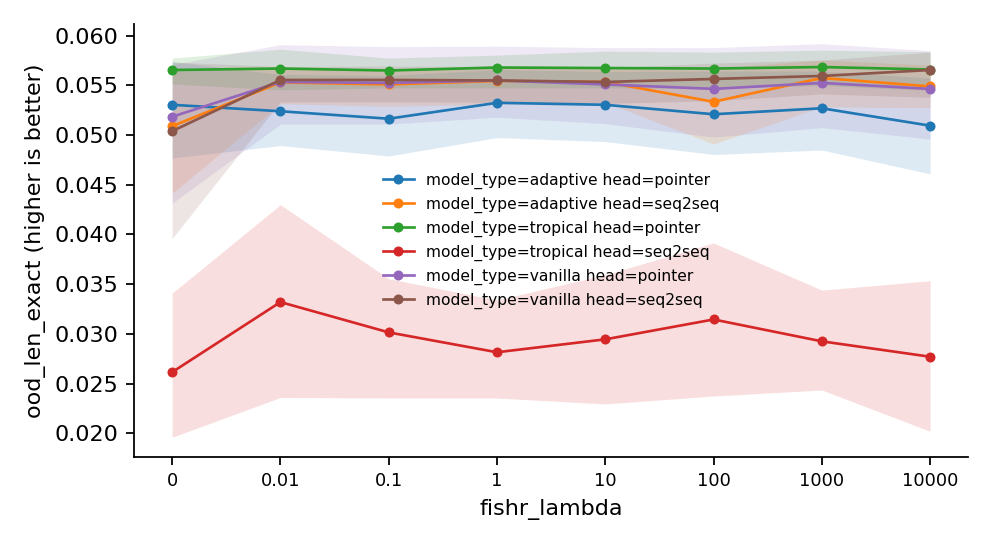
\includegraphics[width=\textwidth]{metric_ood_len_exact.png}
\caption{\texttt{ood\_len\_exact} against \texttt{fishr\_lambda}: the mean over seeds with a 95\% bootstrap CI, one line per combination of the other factors.}
\label{fig:ood_len_exact}
\end{figure}

{\small
\begin{longtable}{lllrlrrr}
\caption{\texttt{ood\_len\_exact} per cell: mean, 95\% bootstrap CI, SD, seeds, diverged runs.}\label{tab:summary-ood_len_exact}\\
\toprule
\texttt{model\_type} & \texttt{head} & \texttt{fishr\_lambda} & mean & 95\% CI & SD & $n$ & div.\\
\midrule
\endhead
adaptive & pointer & 0 & 0.05305 & [0.0477, 0.0574] & 0.0065 & 5 & 0\\
adaptive & pointer & 0.01 & 0.0524 & [0.0489, 0.0561] & 0.00479 & 5 & 0\\
adaptive & pointer & 0.1 & 0.05165 & [0.0479, 0.056] & 0.00525 & 5 & 0\\
adaptive & pointer & 1 & 0.05325 & [0.0497, 0.0566] & 0.00443 & 5 & 0\\
adaptive & pointer & 10 & 0.05305 & [0.0493, 0.0564] & 0.00472 & 5 & 0\\
adaptive & pointer & 100 & 0.0521 & [0.048, 0.0565] & 0.00548 & 5 & 0\\
adaptive & pointer & 1000 & 0.0527 & [0.0485, 0.0565] & 0.00498 & 5 & 0\\
adaptive & pointer & 1e+04 & 0.05095 & [0.0461, 0.0557] & 0.00634 & 5 & 0\\
adaptive & seq2seq & 0 & 0.0509 & [0.0442, 0.0566] & 0.0079 & 5 & 0\\
adaptive & seq2seq & 0.01 & 0.0553 & [0.0531, 0.0568] & 0.00241 & 5 & 0\\
adaptive & seq2seq & 0.1 & 0.0551 & [0.0529, 0.0566] & 0.00245 & 5 & 0\\
adaptive & seq2seq & 1 & 0.05545 & [0.0531, 0.057] & 0.00259 & 5 & 0\\
adaptive & seq2seq & 10 & 0.05535 & [0.0533, 0.0568] & 0.00243 & 5 & 0\\
adaptive & seq2seq & 100 & 0.05335 & [0.0491, 0.0568] & 0.00492 & 5 & 0\\
adaptive & seq2seq & 1000 & 0.05575 & [0.0529, 0.0576] & 0.00315 & 5 & 0\\
adaptive & seq2seq & 1e+04 & 0.0549 & [0.0527, 0.0571] & 0.00281 & 5 & 0\\
tropical & pointer & 0 & 0.05655 & [0.0551, 0.0578] & 0.0018 & 5 & 0\\
tropical & pointer & 0.01 & 0.0567 & [0.0546, 0.0587] & 0.00274 & 5 & 0\\
tropical & pointer & 0.1 & 0.0565 & [0.0548, 0.0578] & 0.00197 & 5 & 0\\
tropical & pointer & 1 & 0.0568 & [0.0548, 0.0581] & 0.00229 & 5 & 0\\
tropical & pointer & 10 & 0.05675 & [0.0548, 0.0585] & 0.00237 & 5 & 0\\
tropical & pointer & 100 & 0.0567 & [0.0547, 0.0583] & 0.00239 & 5 & 0\\
tropical & pointer & 1000 & 0.05685 & [0.055, 0.0586] & 0.0024 & 5 & 0\\
tropical & pointer & 1e+04 & 0.0566 & [0.0545, 0.0584] & 0.0025 & 5 & 0\\
tropical & seq2seq & 0 & 0.02615 & [0.0196, 0.0341] & 0.0091 & 5 & 0\\
tropical & seq2seq & 0.01 & 0.0332 & [0.0236, 0.043] & 0.0129 & 5 & 0\\
tropical & seq2seq & 0.1 & 0.03015 & [0.0236, 0.0355] & 0.00753 & 5 & 0\\
tropical & seq2seq & 1 & 0.02815 & [0.0235, 0.0334] & 0.00654 & 5 & 0\\
tropical & seq2seq & 10 & 0.02945 & [0.0229, 0.036] & 0.00834 & 5 & 0\\
tropical & seq2seq & 100 & 0.03145 & [0.0238, 0.0391] & 0.0102 & 5 & 0\\
tropical & seq2seq & 1000 & 0.02925 & [0.0244, 0.0344] & 0.0066 & 5 & 0\\
tropical & seq2seq & 1e+04 & 0.0277 & [0.0202, 0.0354] & 0.0112 & 5 & 0\\
vanilla & pointer & 0 & 0.05185 & [0.0432, 0.0571] & 0.00945 & 5 & 0\\
vanilla & pointer & 0.01 & 0.05535 & [0.0511, 0.0591] & 0.00515 & 5 & 0\\
vanilla & pointer & 0.1 & 0.05525 & [0.0511, 0.0589] & 0.00494 & 5 & 0\\
vanilla & pointer & 1 & 0.0555 & [0.0518, 0.0589] & 0.00457 & 5 & 0\\
vanilla & pointer & 10 & 0.0551 & [0.0511, 0.0588] & 0.00513 & 5 & 0\\
vanilla & pointer & 100 & 0.05465 & [0.0498, 0.0588] & 0.00601 & 5 & 0\\
vanilla & pointer & 1000 & 0.05525 & [0.0507, 0.0592] & 0.00543 & 5 & 0\\
vanilla & pointer & 1e+04 & 0.05465 & [0.0496, 0.0585] & 0.00577 & 5 & 0\\
vanilla & seq2seq & 0 & 0.0504 & [0.0396, 0.0573] & 0.0121 & 5 & 0\\
vanilla & seq2seq & 0.01 & 0.05555 & [0.0533, 0.0569] & 0.00245 & 5 & 0\\
vanilla & seq2seq & 0.1 & 0.05555 & [0.0533, 0.057] & 0.00244 & 5 & 0\\
vanilla & seq2seq & 1 & 0.0555 & [0.0533, 0.0569] & 0.00241 & 5 & 0\\
vanilla & seq2seq & 10 & 0.05535 & [0.0532, 0.0568] & 0.00235 & 5 & 0\\
vanilla & seq2seq & 100 & 0.05565 & [0.0534, 0.0573] & 0.00258 & 5 & 0\\
vanilla & seq2seq & 1000 & 0.05595 & [0.0541, 0.0576] & 0.00225 & 5 & 0\\
vanilla & seq2seq & 1e+04 & 0.05655 & [0.0538, 0.0584] & 0.00308 & 5 & 0\\
\bottomrule
\end{longtable}
}

{\small
\begin{longtable}{lllrrrl}
\caption{\texttt{ood\_len\_exact}: each level of \texttt{fishr\_lambda} against its control (0), within each combination of the other factors. parametric: Dunnett vs control.}\label{tab:control-ood_len_exact}\\
\toprule
\texttt{model\_type} & \texttt{head} & \texttt{fishr\_lambda} & difference & 95\% CI & $p$ & \\
\midrule
\endhead
adaptive & pointer & 0.01 & $-6.500\times10^{-4}$ & [-0.01, 0.00871] & 1.0000 & \\
adaptive & pointer & 0.1 & -0.0014 & [-0.0108, 0.00796] & 0.9985 & \\
adaptive & pointer & 1 & $2.000\times10^{-4}$ & [-0.00916, 0.00956] & 1.0000 & \\
adaptive & pointer & 10 & 0 & [-0.00936, 0.00936] & 1.0000 & \\
adaptive & pointer & 100 & $-9.500\times10^{-4}$ & [-0.0103, 0.00841] & 0.9999 & \\
adaptive & pointer & 1000 & $-3.500\times10^{-4}$ & [-0.00971, 0.00901] & 1.0000 & \\
adaptive & pointer & 1e+04 & -0.0021 & [-0.0115, 0.00726] & 0.9843 & \\
adaptive & seq2seq & 0.01 & 0.0044 & [-0.00261, 0.0114] & 0.3701 & \\
adaptive & seq2seq & 0.1 & 0.0042 & [-0.00281, 0.0112] & 0.4170 & \\
adaptive & seq2seq & 1 & 0.00455 & [-0.00246, 0.0116] & 0.3371 & \\
adaptive & seq2seq & 10 & 0.00445 & [-0.00256, 0.0115] & 0.3589 & \\
adaptive & seq2seq & 100 & 0.00245 & [-0.00456, 0.00946] & 0.8728 & \\
adaptive & seq2seq & 1000 & 0.00485 & [-0.00216, 0.0119] & 0.2770 & \\
adaptive & seq2seq & 1e+04 & 0.004 & [-0.00301, 0.011] & 0.4671 & \\
tropical & pointer & 0.01 & $1.500\times10^{-4}$ & [-0.00391, 0.00421] & 1.0000 & \\
tropical & pointer & 0.1 & $-5.000\times10^{-5}$ & [-0.00411, 0.00401] & 1.0000 & \\
tropical & pointer & 1 & $2.500\times10^{-4}$ & [-0.00381, 0.00431] & 1.0000 & \\
tropical & pointer & 10 & $2.000\times10^{-4}$ & [-0.00386, 0.00426] & 1.0000 & \\
tropical & pointer & 100 & $1.500\times10^{-4}$ & [-0.00391, 0.00421] & 1.0000 & \\
tropical & pointer & 1000 & $3.000\times10^{-4}$ & [-0.00376, 0.00436] & 1.0000 & \\
tropical & pointer & 1e+04 & $5.000\times10^{-5}$ & [-0.00401, 0.00411] & 1.0000 & \\
tropical & seq2seq & 0.01 & 0.00705 & [-0.00918, 0.0233] & 0.7291 & \\
tropical & seq2seq & 0.1 & 0.004 & [-0.0122, 0.0202] & 0.9743 & \\
tropical & seq2seq & 1 & 0.002 & [-0.0142, 0.0182] & 0.9996 & \\
tropical & seq2seq & 10 & 0.0033 & [-0.0129, 0.0195] & 0.9909 & \\
tropical & seq2seq & 100 & 0.0053 & [-0.0109, 0.0215] & 0.9037 & \\
tropical & seq2seq & 1000 & 0.0031 & [-0.0131, 0.0193] & 0.9937 & \\
tropical & seq2seq & 1e+04 & 0.00155 & [-0.0147, 0.0178] & 0.9999 & \\
vanilla & pointer & 0.01 & 0.0035 & [-0.00695, 0.0139] & 0.8929 & \\
vanilla & pointer & 0.1 & 0.0034 & [-0.00705, 0.0138] & 0.9051 & \\
vanilla & pointer & 1 & 0.00365 & [-0.0068, 0.0141] & 0.8733 & \\
vanilla & pointer & 10 & 0.00325 & [-0.0072, 0.0137] & 0.9218 & \\
vanilla & pointer & 100 & 0.0028 & [-0.00765, 0.0132] & 0.9608 & \\
vanilla & pointer & 1000 & 0.0034 & [-0.00705, 0.0138] & 0.9051 & \\
vanilla & pointer & 1e+04 & 0.0028 & [-0.00765, 0.0132] & 0.9608 & \\
vanilla & seq2seq & 0.01 & 0.00515 & [-0.00341, 0.0137] & 0.4130 & \\
vanilla & seq2seq & 0.1 & 0.00515 & [-0.00341, 0.0137] & 0.4129 & \\
vanilla & seq2seq & 1 & 0.0051 & [-0.00346, 0.0137] & 0.4229 & \\
vanilla & seq2seq & 10 & 0.00495 & [-0.00361, 0.0135] & 0.4535 & \\
vanilla & seq2seq & 100 & 0.00525 & [-0.00331, 0.0138] & 0.3934 & \\
vanilla & seq2seq & 1000 & 0.00555 & [-0.00301, 0.0141] & 0.3383 & \\
vanilla & seq2seq & 1e+04 & 0.00615 & [-0.00241, 0.0147] & 0.2439 & \\
\bottomrule
\end{longtable}
}

{\small
\begin{longtable}{llrrrrr}
\caption{\texttt{ood\_len\_exact} against log10 \texttt{fishr\_lambda}: parametric: OLS slope t-test, seed-bootstrap CI, with the Jonckheere--Terpstra ordered-trend $\tau$ and $p$.}\label{tab:trend-ood_len_exact}\\
\toprule
\texttt{model\_type} & \texttt{head} & estimate & 95\% CI & $p$ & JT $\tau$ & JT $p$\\
\midrule
\endhead
adaptive & pointer & $-1.214\times10^{-4}$ & [$-3.84\times10^{-4}$, $1.79\times10^{-5}$] & 0.7675 & -0.0248 & 0.8664\\
adaptive & seq2seq & $-7.143\times10^{-5}$ & [$-1.86\times10^{-4}$, $2.14\times10^{-5}$] & 0.7749 & 0.0819 & 0.5397\\
tropical & pointer & $1.071\times10^{-5}$ & [$-3.57\times10^{-5}$, $6.07\times10^{-5}$] & 0.9545 & 0.0152 & 0.9150\\
tropical & seq2seq & $-5.357\times10^{-4}$ & [-0.00169, $6.00\times10^{-4}$] & 0.4718 & -0.0762 & 0.5745\\
vanilla & pointer & $-1.054\times10^{-4}$ & [$-3.00\times10^{-4}$, $4.82\times10^{-5}$] & 0.8005 & -0.0248 & 0.8580\\
vanilla & seq2seq & $1.411\times10^{-4}$ & [$6.61\times10^{-5}$, $2.11\times10^{-4}$] & 0.4798 & 0.137 & 0.2939\\
\bottomrule
\end{longtable}
}

{\small
\begin{longtable}{lrrrl}
\caption{\texttt{ood\_len\_exact}: paired contrasts by seed, Holm-corrected across the cells. parametric: paired t-test by seed, Holm.}\label{tab:paired-ood_len_exact}\\
\toprule
contrast (within) & difference & 95\% CI & $p$ & \\
\midrule
\endhead
\stackcell{model\_type: tropical - vanilla\\\footnotesize head=pointer fishr\_lambda=0 } & 0.0047 & [-0.00821, 0.0176] & 1.0000 & \\
\stackcell{model\_type: tropical - vanilla\\\footnotesize head=pointer fishr\_lambda=0.01 } & 0.00135 & [-0.00345, 0.00615] & 1.0000 & \\
\stackcell{model\_type: tropical - vanilla\\\footnotesize head=pointer fishr\_lambda=0.1 } & 0.00125 & [-0.00377, 0.00627] & 1.0000 & \\
\stackcell{model\_type: tropical - vanilla\\\footnotesize head=pointer fishr\_lambda=1 } & 0.0013 & [-0.00369, 0.00629] & 1.0000 & \\
\stackcell{model\_type: tropical - vanilla\\\footnotesize head=pointer fishr\_lambda=10 } & 0.00165 & [-0.00421, 0.00751] & 1.0000 & \\
\stackcell{model\_type: tropical - vanilla\\\footnotesize head=pointer fishr\_lambda=100 } & 0.00205 & [-0.00435, 0.00845] & 1.0000 & \\
\stackcell{model\_type: tropical - vanilla\\\footnotesize head=pointer fishr\_lambda=1000 } & 0.0016 & [-0.00375, 0.00695] & 1.0000 & \\
\stackcell{model\_type: tropical - vanilla\\\footnotesize head=pointer fishr\_lambda=1e+04 } & 0.00195 & [-0.00403, 0.00793] & 1.0000 & \\
\stackcell{model\_type: tropical - vanilla\\\footnotesize head=seq2seq fishr\_lambda=0 } & -0.02425 & [-0.0405, -0.00797] & 0.1442 & \\
\stackcell{model\_type: tropical - vanilla\\\footnotesize head=seq2seq fishr\_lambda=0.01 } & -0.02235 & [-0.0398, -0.00492] & 0.2122 & \\
\stackcell{model\_type: tropical - vanilla\\\footnotesize head=seq2seq fishr\_lambda=0.1 } & -0.0254 & [-0.0367, -0.0141] & 0.0419 & *\\
\stackcell{model\_type: tropical - vanilla\\\footnotesize head=seq2seq fishr\_lambda=1 } & -0.02735 & [-0.0372, -0.0175] & 0.0226 & *\\
\stackcell{model\_type: tropical - vanilla\\\footnotesize head=seq2seq fishr\_lambda=10 } & -0.0259 & [-0.0364, -0.0154] & 0.0333 & *\\
\stackcell{model\_type: tropical - vanilla\\\footnotesize head=seq2seq fishr\_lambda=100 } & -0.0242 & [-0.0374, -0.011] & 0.0776 & \\
\stackcell{model\_type: tropical - vanilla\\\footnotesize head=seq2seq fishr\_lambda=1000 } & -0.0267 & [-0.0358, -0.0176] & 0.0200 & *\\
\stackcell{model\_type: tropical - vanilla\\\footnotesize head=seq2seq fishr\_lambda=1e+04 } & -0.02885 & [-0.0415, -0.0162] & 0.0419 & *\\
\stackcell{model\_type: adaptive - vanilla\\\footnotesize head=pointer fishr\_lambda=0 } & 0.0012 & [-0.00329, 0.00569] & 1.0000 & \\
\stackcell{model\_type: adaptive - vanilla\\\footnotesize head=pointer fishr\_lambda=0.01 } & -0.00295 & [-0.0127, 0.00678] & 1.0000 & \\
\stackcell{model\_type: adaptive - vanilla\\\footnotesize head=pointer fishr\_lambda=0.1 } & -0.0036 & [-0.0136, 0.0064] & 1.0000 & \\
\stackcell{model\_type: adaptive - vanilla\\\footnotesize head=pointer fishr\_lambda=1 } & -0.00225 & [-0.0114, 0.00686] & 1.0000 & \\
\stackcell{model\_type: adaptive - vanilla\\\footnotesize head=pointer fishr\_lambda=10 } & -0.00205 & [-0.0122, 0.00807] & 1.0000 & \\
\stackcell{model\_type: adaptive - vanilla\\\footnotesize head=pointer fishr\_lambda=100 } & -0.00255 & [-0.0144, 0.00932] & 1.0000 & \\
\stackcell{model\_type: adaptive - vanilla\\\footnotesize head=pointer fishr\_lambda=1000 } & -0.00255 & [-0.0129, 0.0078] & 1.0000 & \\
\stackcell{model\_type: adaptive - vanilla\\\footnotesize head=pointer fishr\_lambda=1e+04 } & -0.0037 & [-0.0152, 0.00781] & 1.0000 & \\
\stackcell{model\_type: adaptive - vanilla\\\footnotesize head=seq2seq fishr\_lambda=0 } & $5.000\times10^{-4}$ & [-0.019, 0.02] & 1.0000 & \\
\stackcell{model\_type: adaptive - vanilla\\\footnotesize head=seq2seq fishr\_lambda=0.01 } & $-2.500\times10^{-4}$ & [$-9.78\times10^{-4}$, $4.78\times10^{-4}$] & 1.0000 & \\
\stackcell{model\_type: adaptive - vanilla\\\footnotesize head=seq2seq fishr\_lambda=0.1 } & $-4.500\times10^{-4}$ & [-0.00105, $1.47\times10^{-4}$] & 1.0000 & \\
\stackcell{model\_type: adaptive - vanilla\\\footnotesize head=seq2seq fishr\_lambda=1 } & $-5.000\times10^{-5}$ & [$-6.47\times10^{-4}$, $5.47\times10^{-4}$] & 1.0000 & \\
\stackcell{model\_type: adaptive - vanilla\\\footnotesize head=seq2seq fishr\_lambda=10 } & 0 & [$-5.81\times10^{-4}$, $5.81\times10^{-4}$] & 1.0000 & \\
\stackcell{model\_type: adaptive - vanilla\\\footnotesize head=seq2seq fishr\_lambda=100 } & -0.0023 & [-0.00805, 0.00345] & 1.0000 & \\
\stackcell{model\_type: adaptive - vanilla\\\footnotesize head=seq2seq fishr\_lambda=1000 } & $-2.000\times10^{-4}$ & [-0.00249, 0.00209] & 1.0000 & \\
\stackcell{model\_type: adaptive - vanilla\\\footnotesize head=seq2seq fishr\_lambda=1e+04 } & -0.00165 & [-0.0049, 0.0016] & 1.0000 & \\
\stackcell{head: pointer - seq2seq\\\footnotesize model\_type=adaptive fishr\_lambda=0 } & 0.00215 & [-0.0116, 0.0159] & 1.0000 & \\
\stackcell{head: pointer - seq2seq\\\footnotesize model\_type=adaptive fishr\_lambda=0.01 } & -0.0029 & [-0.00982, 0.00402] & 1.0000 & \\
\stackcell{head: pointer - seq2seq\\\footnotesize model\_type=adaptive fishr\_lambda=0.1 } & -0.00345 & [-0.0108, 0.00389] & 1.0000 & \\
\stackcell{head: pointer - seq2seq\\\footnotesize model\_type=adaptive fishr\_lambda=1 } & -0.0022 & [-0.0093, 0.0049] & 1.0000 & \\
\stackcell{head: pointer - seq2seq\\\footnotesize model\_type=adaptive fishr\_lambda=10 } & -0.0023 & [-0.0098, 0.0052] & 1.0000 & \\
\stackcell{head: pointer - seq2seq\\\footnotesize model\_type=adaptive fishr\_lambda=100 } & -0.00125 & [-0.0129, 0.0104] & 1.0000 & \\
\stackcell{head: pointer - seq2seq\\\footnotesize model\_type=adaptive fishr\_lambda=1000 } & -0.00305 & [-0.0107, 0.00462] & 1.0000 & \\
\stackcell{head: pointer - seq2seq\\\footnotesize model\_type=adaptive fishr\_lambda=1e+04 } & -0.00395 & [-0.0119, 0.00399] & 1.0000 & \\
\stackcell{head: pointer - seq2seq\\\footnotesize model\_type=tropical fishr\_lambda=0 } & 0.0304 & [0.0192, 0.0416] & 0.0366 & *\\
\stackcell{head: pointer - seq2seq\\\footnotesize model\_type=tropical fishr\_lambda=0.01 } & 0.0235 & [0.00705, 0.04] & 0.2821 & \\
\stackcell{head: pointer - seq2seq\\\footnotesize model\_type=tropical fishr\_lambda=0.1 } & 0.02635 & [0.0156, 0.0371] & 0.0480 & *\\
\stackcell{head: pointer - seq2seq\\\footnotesize model\_type=tropical fishr\_lambda=1 } & 0.02865 & [0.0188, 0.0385] & 0.0293 & *\\
\stackcell{head: pointer - seq2seq\\\footnotesize model\_type=tropical fishr\_lambda=10 } & 0.0273 & [0.0166, 0.038] & 0.0435 & *\\
\stackcell{head: pointer - seq2seq\\\footnotesize model\_type=tropical fishr\_lambda=100 } & 0.02525 & [0.0112, 0.0393] & 0.1374 & \\
\stackcell{head: pointer - seq2seq\\\footnotesize model\_type=tropical fishr\_lambda=1000 } & 0.0276 & [0.02, 0.0352] & 0.0133 & *\\
\stackcell{head: pointer - seq2seq\\\footnotesize model\_type=tropical fishr\_lambda=1e+04 } & 0.0289 & [0.0147, 0.0431] & 0.0911 & \\
\stackcell{head: pointer - seq2seq\\\footnotesize model\_type=vanilla fishr\_lambda=0 } & 0.00145 & [-0.0209, 0.0238] & 1.0000 & \\
\stackcell{head: pointer - seq2seq\\\footnotesize model\_type=vanilla fishr\_lambda=0.01 } & $-2.000\times10^{-4}$ & [-0.0063, 0.0059] & 1.0000 & \\
\stackcell{head: pointer - seq2seq\\\footnotesize model\_type=vanilla fishr\_lambda=0.1 } & $-3.000\times10^{-4}$ & [-0.00596, 0.00536] & 1.0000 & \\
\stackcell{head: pointer - seq2seq\\\footnotesize model\_type=vanilla fishr\_lambda=1 } & $-1.388\times10^{-18}$ & [-0.00534, 0.00534] & 1.0000 & \\
\stackcell{head: pointer - seq2seq\\\footnotesize model\_type=vanilla fishr\_lambda=10 } & $-2.500\times10^{-4}$ & [-0.00621, 0.00571] & 1.0000 & \\
\stackcell{head: pointer - seq2seq\\\footnotesize model\_type=vanilla fishr\_lambda=100 } & -0.001 & [-0.00919, 0.00719] & 1.0000 & \\
\stackcell{head: pointer - seq2seq\\\footnotesize model\_type=vanilla fishr\_lambda=1000 } & $-7.000\times10^{-4}$ & [-0.00631, 0.00491] & 1.0000 & \\
\stackcell{head: pointer - seq2seq\\\footnotesize model\_type=vanilla fishr\_lambda=1e+04 } & -0.0019 & [-0.00967, 0.00587] & 1.0000 & \\
\bottomrule
\end{longtable}
}

\subsection{\texttt{ood\_val\_f1}}
\begin{figure}[tbp]
\centering
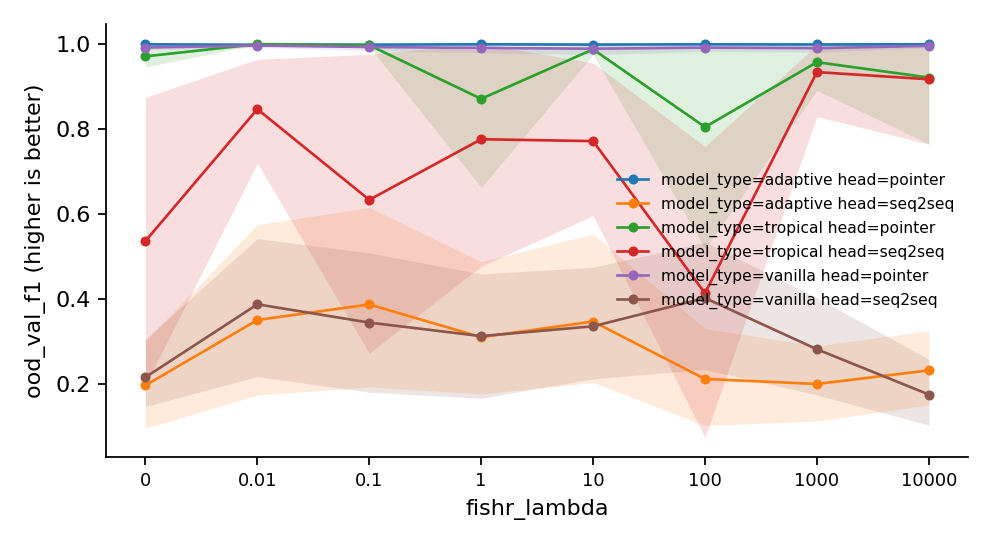
\includegraphics[width=\textwidth]{metric_ood_val_f1.png}
\caption{\texttt{ood\_val\_f1} against \texttt{fishr\_lambda}: the mean over seeds with a 95\% bootstrap CI, one line per combination of the other factors.}
\label{fig:ood_val_f1}
\end{figure}

{\small
\begin{longtable}{lllrlrrr}
\caption{\texttt{ood\_val\_f1} per cell: mean, 95\% bootstrap CI, SD, seeds, diverged runs.}\label{tab:summary-ood_val_f1}\\
\toprule
\texttt{model\_type} & \texttt{head} & \texttt{fishr\_lambda} & mean & 95\% CI & SD & $n$ & div.\\
\midrule
\endhead
adaptive & pointer & 0 & 0.9985 & [0.996, 1] & 0.00289 & 5 & 0\\
adaptive & pointer & 0.01 & 0.9975 & [0.995, 1] & 0.00294 & 5 & 0\\
adaptive & pointer & 0.1 & 0.9977 & [0.996, 1] & 0.00243 & 5 & 0\\
adaptive & pointer & 1 & 0.9985 & [0.997, 1] & 0.00204 & 5 & 0\\
adaptive & pointer & 10 & 0.9979 & [0.996, 1] & 0.00259 & 5 & 0\\
adaptive & pointer & 100 & 0.9985 & [0.997, 1] & 0.00192 & 5 & 0\\
adaptive & pointer & 1000 & 0.9981 & [0.996, 0.999] & 0.00199 & 5 & 0\\
adaptive & pointer & 1e+04 & 0.9987 & [0.997, 1] & 0.00169 & 5 & 0\\
adaptive & seq2seq & 0 & 0.1969 & [0.0961, 0.301] & 0.133 & 5 & 0\\
adaptive & seq2seq & 0.01 & 0.3504 & [0.174, 0.575] & 0.258 & 5 & 0\\
adaptive & seq2seq & 0.1 & 0.3871 & [0.193, 0.615] & 0.255 & 5 & 0\\
adaptive & seq2seq & 1 & 0.3101 & [0.177, 0.488] & 0.211 & 5 & 0\\
adaptive & seq2seq & 10 & 0.3469 & [0.204, 0.552] & 0.233 & 5 & 0\\
adaptive & seq2seq & 100 & 0.2118 & [0.102, 0.33] & 0.151 & 5 & 0\\
adaptive & seq2seq & 1000 & 0.2001 & [0.113, 0.29] & 0.114 & 5 & 0\\
adaptive & seq2seq & 1e+04 & 0.2321 & [0.151, 0.325] & 0.114 & 5 & 0\\
tropical & pointer & 0 & 0.9702 & [0.945, 0.996] & 0.033 & 5 & 0\\
tropical & pointer & 0.01 & 0.999 & [0.998, 1] & 0.00104 & 5 & 0\\
tropical & pointer & 0.1 & 0.9965 & [0.993, 0.999] & 0.00425 & 5 & 0\\
tropical & pointer & 1 & 0.8704 & [0.662, 0.985] & 0.23 & 5 & 0\\
tropical & pointer & 10 & 0.9867 & [0.974, 0.996] & 0.0143 & 5 & 0\\
tropical & pointer & 100 & 0.804 & [0.518, 0.993] & 0.311 & 5 & 0\\
tropical & pointer & 1000 & 0.9565 & [0.89, 1] & 0.0785 & 5 & 0\\
tropical & pointer & 1e+04 & 0.9204 & [0.765, 0.999] & 0.174 & 5 & 0\\
tropical & seq2seq & 0 & 0.5362 & [0.198, 0.874] & 0.445 & 5 & 0\\
tropical & seq2seq & 0.01 & 0.8461 & [0.719, 0.963] & 0.167 & 5 & 0\\
tropical & seq2seq & 0.1 & 0.633 & [0.272, 0.975] & 0.455 & 5 & 0\\
tropical & seq2seq & 1 & 0.7754 & [0.477, 1] & 0.334 & 5 & 0\\
tropical & seq2seq & 10 & 0.7709 & [0.596, 0.955] & 0.23 & 5 & 0\\
tropical & seq2seq & 100 & 0.4134 & [0.0748, 0.758] & 0.44 & 5 & 0\\
tropical & seq2seq & 1000 & 0.9332 & [0.829, 0.997] & 0.115 & 5 & 0\\
tropical & seq2seq & 1e+04 & 0.9163 & [0.764, 1] & 0.167 & 5 & 0\\
vanilla & pointer & 0 & 0.9909 & [0.985, 0.997] & 0.00773 & 5 & 0\\
vanilla & pointer & 0.01 & 0.9956 & [0.991, 0.999] & 0.0052 & 5 & 0\\
vanilla & pointer & 0.1 & 0.9922 & [0.984, 1] & 0.0108 & 5 & 0\\
vanilla & pointer & 1 & 0.99 & [0.979, 0.999] & 0.013 & 5 & 0\\
vanilla & pointer & 10 & 0.9882 & [0.974, 0.999] & 0.016 & 5 & 0\\
vanilla & pointer & 100 & 0.9908 & [0.982, 1] & 0.0118 & 5 & 0\\
vanilla & pointer & 1000 & 0.9894 & [0.98, 0.998] & 0.0119 & 5 & 0\\
vanilla & pointer & 1e+04 & 0.995 & [0.99, 0.999] & 0.00584 & 5 & 0\\
vanilla & seq2seq & 0 & 0.2159 & [0.147, 0.306] & 0.105 & 5 & 0\\
vanilla & seq2seq & 0.01 & 0.3873 & [0.217, 0.542] & 0.209 & 5 & 0\\
vanilla & seq2seq & 0.1 & 0.3444 & [0.181, 0.508] & 0.21 & 5 & 0\\
vanilla & seq2seq & 1 & 0.3126 & [0.166, 0.459] & 0.191 & 5 & 0\\
vanilla & seq2seq & 10 & 0.3357 & [0.212, 0.474] & 0.17 & 5 & 0\\
vanilla & seq2seq & 100 & 0.4021 & [0.234, 0.533] & 0.191 & 5 & 0\\
vanilla & seq2seq & 1000 & 0.2817 & [0.174, 0.403] & 0.147 & 5 & 0\\
vanilla & seq2seq & 1e+04 & 0.1753 & [0.103, 0.258] & 0.0989 & 5 & 0\\
\bottomrule
\end{longtable}
}

{\small
\begin{longtable}{lllrrrl}
\caption{\texttt{ood\_val\_f1}: each level of \texttt{fishr\_lambda} against its control (0), within each combination of the other factors. rank: Wilcoxon signed-rank by seed, Holm.}\label{tab:control-ood_val_f1}\\
\toprule
\texttt{model\_type} & \texttt{head} & \texttt{fishr\_lambda} & difference & 95\% CI & $p$ & \\
\midrule
\endhead
adaptive & pointer & 0.01 & $-5.508\times10^{-4}$ & [-0.00218, $2.50\times10^{-5}$] & 1.0000 & \\
adaptive & pointer & 0.1 & $-2.874\times10^{-4}$ & [-0.00316, 0.00128] & 1.0000 & \\
adaptive & pointer & 1 & $-9.610\times10^{-5}$ & [$-9.38\times10^{-4}$, 0.00101] & 1.0000 & \\
adaptive & pointer & 10 & $-9.270\times10^{-5}$ & [-0.00165, $3.30\times10^{-4}$] & 1.0000 & \\
adaptive & pointer & 100 & $-1.298\times10^{-4}$ & [$-9.13\times10^{-4}$, $9.72\times10^{-4}$] & 1.0000 & \\
adaptive & pointer & 1000 & $-3.555\times10^{-4}$ & [-0.00143, $7.50\times10^{-4}$] & 1.0000 & \\
adaptive & pointer & 1e+04 & $3.090\times10^{-6}$ & [-0.0019, 0.00222] & 1.0000 & \\
adaptive & seq2seq & 0.01 & 0.1463 & [-0.0287, 0.342] & 1.0000 & \\
adaptive & seq2seq & 0.1 & 0.1325 & [-0.0157, 0.391] & 1.0000 & \\
adaptive & seq2seq & 1 & 0.1006 & [-0.0173, 0.25] & 1.0000 & \\
adaptive & seq2seq & 10 & 0.1654 & [$-2.31\times10^{-4}$, 0.304] & 1.0000 & \\
adaptive & seq2seq & 100 & -0.05391 & [-0.154, 0.218] & 1.0000 & \\
adaptive & seq2seq & 1000 & $-1.478\times10^{-4}$ & [-0.11, 0.151] & 1.0000 & \\
adaptive & seq2seq & 1e+04 & -0.0307 & [-0.129, 0.202] & 1.0000 & \\
tropical & pointer & 0.01 & 0.01565 & [0.00311, 0.0544] & 1.0000 & \\
tropical & pointer & 0.1 & 0.0154 & [0.00366, 0.0489] & 0.8750 & \\
tropical & pointer & 1 & -0.03139 & [-0.299, 0.0236] & 1.0000 & \\
tropical & pointer & 10 & 0.01558 & [-0.00208, 0.0368] & 1.0000 & \\
tropical & pointer & 100 & -0.006786 & [-0.429, 0.0214] & 1.0000 & \\
tropical & pointer & 1000 & 0.0157 & [-0.101, 0.0545] & 1.0000 & \\
tropical & pointer & 1e+04 & 0.01528 & [-0.221, 0.0543] & 1.0000 & \\
tropical & seq2seq & 0.01 & 0.2234 & [0.0447, 0.591] & 1.0000 & \\
tropical & seq2seq & 0.1 & 0 & [-0.158, 0.403] & 1.0000 & \\
tropical & seq2seq & 1 & 0 & [-0.0465, 0.638] & 1.0000 & \\
tropical & seq2seq & 10 & 0.2554 & [-0.185, 0.678] & 1.0000 & \\
tropical & seq2seq & 100 & 0 & [-0.572, 0.218] & 1.0000 & \\
tropical & seq2seq & 1000 & 0.3605 & [0.072, 0.729] & 1.0000 & \\
tropical & seq2seq & 1e+04 & 0.2485 & [0.0495, 0.729] & 1.0000 & \\
vanilla & pointer & 0.01 & 0.004756 & [-0.0037, 0.0128] & 1.0000 & \\
vanilla & pointer & 0.1 & $1.215\times10^{-4}$ & [-0.0096, 0.0121] & 1.0000 & \\
vanilla & pointer & 1 & $1.588\times10^{-4}$ & [-0.0126, 0.0116] & 1.0000 & \\
vanilla & pointer & 10 & $-5.296\times10^{-5}$ & [-0.0199, 0.0108] & 1.0000 & \\
vanilla & pointer & 100 & $4.984\times10^{-5}$ & [-0.0123, 0.0119] & 1.0000 & \\
vanilla & pointer & 1000 & $2.336\times10^{-4}$ & [-0.0128, 0.0104] & 1.0000 & \\
vanilla & pointer & 1e+04 & $1.464\times10^{-4}$ & [-0.00351, 0.0117] & 1.0000 & \\
vanilla & seq2seq & 0.01 & 0.1753 & [0.0564, 0.289] & 0.4375 & \\
vanilla & seq2seq & 0.1 & 0.05913 & [0.0214, 0.277] & 0.5000 & \\
vanilla & seq2seq & 1 & 0.005633 & [0.00382, 0.201] & 0.4375 & \\
vanilla & seq2seq & 10 & 0.1114 & [0.0491, 0.19] & 0.4375 & \\
vanilla & seq2seq & 100 & 0.1501 & [0.0778, 0.294] & 0.5000 & \\
vanilla & seq2seq & 1000 & 0.02088 & [0.00523, 0.144] & 0.5000 & \\
vanilla & seq2seq & 1e+04 & -0.03068 & [-0.166, 0.0607] & 1.0000 & \\
\bottomrule
\end{longtable}
}

{\small
\begin{longtable}{llrrrrr}
\caption{\texttt{ood\_val\_f1} against log10 \texttt{fishr\_lambda}: rank: Spearman rho, seed-bootstrap CI, with the Jonckheere--Terpstra ordered-trend $\tau$ and $p$.}\label{tab:trend-ood_val_f1}\\
\toprule
\texttt{model\_type} & \texttt{head} & estimate & 95\% CI & $p$ & JT $\tau$ & JT $p$\\
\midrule
\endhead
adaptive & pointer & 0.1167 & [-0.151, 0.382] & 0.5044 & 0.0838 & 0.5371\\
adaptive & seq2seq & -0.2645 & [-0.682, 0.232] & 0.1247 & -0.2 & 0.1416\\
tropical & pointer & -0.1584 & [-0.567, 0.144] & 0.3634 & -0.131 & 0.3311\\
tropical & seq2seq & 0.1176 & [-0.154, 0.364] & 0.5010 & 0.0857 & 0.5149\\
vanilla & pointer & -0.04526 & [-0.22, 0.132] & 0.7963 & -0.0438 & 0.7552\\
vanilla & seq2seq & -0.2942 & [-0.607, -0.0085] & 0.0862 & -0.234 & 0.0792\\
\bottomrule
\end{longtable}
}

{\small
\begin{longtable}{lrrrl}
\caption{\texttt{ood\_val\_f1}: paired contrasts by seed, Holm-corrected across the cells. rank: Wilcoxon signed-rank by seed, Holm.}\label{tab:paired-ood_val_f1}\\
\toprule
contrast (within) & difference & 95\% CI & $p$ & \\
\midrule
\endhead
\stackcell{model\_type: tropical - vanilla\\\footnotesize head=pointer fishr\_lambda=0 } & -0.02073 & [-0.0578, 0.0163] & 1.0000 & \\
\stackcell{model\_type: tropical - vanilla\\\footnotesize head=pointer fishr\_lambda=0.01 } & 0.003361 & [-0.00377, 0.0105] & 1.0000 & \\
\stackcell{model\_type: tropical - vanilla\\\footnotesize head=pointer fishr\_lambda=0.1 } & 0.004272 & [-0.00687, 0.0154] & 1.0000 & \\
\stackcell{model\_type: tropical - vanilla\\\footnotesize head=pointer fishr\_lambda=1 } & -0.1196 & [-0.412, 0.173] & 1.0000 & \\
\stackcell{model\_type: tropical - vanilla\\\footnotesize head=pointer fishr\_lambda=10 } & -0.001476 & [-0.0295, 0.0265] & 1.0000 & \\
\stackcell{model\_type: tropical - vanilla\\\footnotesize head=pointer fishr\_lambda=100 } & -0.1868 & [-0.581, 0.207] & 1.0000 & \\
\stackcell{model\_type: tropical - vanilla\\\footnotesize head=pointer fishr\_lambda=1000 } & -0.0329 & [-0.124, 0.0582] & 1.0000 & \\
\stackcell{model\_type: tropical - vanilla\\\footnotesize head=pointer fishr\_lambda=1e+04 } & -0.07459 & [-0.287, 0.138] & 1.0000 & \\
\stackcell{model\_type: tropical - vanilla\\\footnotesize head=seq2seq fishr\_lambda=0 } & 0.3202 & [-0.153, 0.793] & 1.0000 & \\
\stackcell{model\_type: tropical - vanilla\\\footnotesize head=seq2seq fishr\_lambda=0.01 } & 0.4588 & [0.118, 0.799] & 1.0000 & \\
\stackcell{model\_type: tropical - vanilla\\\footnotesize head=seq2seq fishr\_lambda=0.1 } & 0.2886 & [-0.159, 0.736] & 1.0000 & \\
\stackcell{model\_type: tropical - vanilla\\\footnotesize head=seq2seq fishr\_lambda=1 } & 0.4628 & [-0.0977, 1.02] & 1.0000 & \\
\stackcell{model\_type: tropical - vanilla\\\footnotesize head=seq2seq fishr\_lambda=10 } & 0.4352 & [0.113, 0.758] & 1.0000 & \\
\stackcell{model\_type: tropical - vanilla\\\footnotesize head=seq2seq fishr\_lambda=100 } & 0.01129 & [-0.378, 0.4] & 1.0000 & \\
\stackcell{model\_type: tropical - vanilla\\\footnotesize head=seq2seq fishr\_lambda=1000 } & 0.6515 & [0.385, 0.919] & 1.0000 & \\
\stackcell{model\_type: tropical - vanilla\\\footnotesize head=seq2seq fishr\_lambda=1e+04 } & 0.7411 & [0.519, 0.963] & 1.0000 & \\
\stackcell{model\_type: adaptive - vanilla\\\footnotesize head=pointer fishr\_lambda=0 } & 0.007566 & [-0.00459, 0.0197] & 1.0000 & \\
\stackcell{model\_type: adaptive - vanilla\\\footnotesize head=pointer fishr\_lambda=0.01 } & 0.001857 & [-0.00114, 0.00485] & 1.0000 & \\
\stackcell{model\_type: adaptive - vanilla\\\footnotesize head=pointer fishr\_lambda=0.1 } & 0.005543 & [-0.0049, 0.016] & 1.0000 & \\
\stackcell{model\_type: adaptive - vanilla\\\footnotesize head=pointer fishr\_lambda=1 } & 0.00854 & [-0.00694, 0.024] & 1.0000 & \\
\stackcell{model\_type: adaptive - vanilla\\\footnotesize head=pointer fishr\_lambda=10 } & 0.009736 & [-0.00735, 0.0268] & 1.0000 & \\
\stackcell{model\_type: adaptive - vanilla\\\footnotesize head=pointer fishr\_lambda=100 } & 0.007635 & [-0.00538, 0.0207] & 1.0000 & \\
\stackcell{model\_type: adaptive - vanilla\\\footnotesize head=pointer fishr\_lambda=1000 } & 0.008737 & [-0.00414, 0.0216] & 1.0000 & \\
\stackcell{model\_type: adaptive - vanilla\\\footnotesize head=pointer fishr\_lambda=1e+04 } & 0.003706 & [-0.00367, 0.0111] & 1.0000 & \\
\stackcell{model\_type: adaptive - vanilla\\\footnotesize head=seq2seq fishr\_lambda=0 } & -0.01903 & [-0.19, 0.152] & 1.0000 & \\
\stackcell{model\_type: adaptive - vanilla\\\footnotesize head=seq2seq fishr\_lambda=0.01 } & -0.03689 & [-0.35, 0.276] & 1.0000 & \\
\stackcell{model\_type: adaptive - vanilla\\\footnotesize head=seq2seq fishr\_lambda=0.1 } & 0.04273 & [-0.304, 0.389] & 1.0000 & \\
\stackcell{model\_type: adaptive - vanilla\\\footnotesize head=seq2seq fishr\_lambda=1 } & -0.002543 & [-0.185, 0.179] & 1.0000 & \\
\stackcell{model\_type: adaptive - vanilla\\\footnotesize head=seq2seq fishr\_lambda=10 } & 0.01123 & [-0.178, 0.2] & 1.0000 & \\
\stackcell{model\_type: adaptive - vanilla\\\footnotesize head=seq2seq fishr\_lambda=100 } & -0.1902 & [-0.473, 0.0927] & 1.0000 & \\
\stackcell{model\_type: adaptive - vanilla\\\footnotesize head=seq2seq fishr\_lambda=1000 } & -0.08162 & [-0.31, 0.146] & 1.0000 & \\
\stackcell{model\_type: adaptive - vanilla\\\footnotesize head=seq2seq fishr\_lambda=1e+04 } & 0.0568 & [-0.152, 0.266] & 1.0000 & \\
\stackcell{head: pointer - seq2seq\\\footnotesize model\_type=adaptive fishr\_lambda=0 } & 0.8016 & [0.635, 0.968] & 1.0000 & \\
\stackcell{head: pointer - seq2seq\\\footnotesize model\_type=adaptive fishr\_lambda=0.01 } & 0.647 & [0.324, 0.97] & 1.0000 & \\
\stackcell{head: pointer - seq2seq\\\footnotesize model\_type=adaptive fishr\_lambda=0.1 } & 0.6106 & [0.293, 0.928] & 1.0000 & \\
\stackcell{head: pointer - seq2seq\\\footnotesize model\_type=adaptive fishr\_lambda=1 } & 0.6885 & [0.425, 0.952] & 1.0000 & \\
\stackcell{head: pointer - seq2seq\\\footnotesize model\_type=adaptive fishr\_lambda=10 } & 0.651 & [0.36, 0.943] & 1.0000 & \\
\stackcell{head: pointer - seq2seq\\\footnotesize model\_type=adaptive fishr\_lambda=100 } & 0.7866 & [0.601, 0.972] & 1.0000 & \\
\stackcell{head: pointer - seq2seq\\\footnotesize model\_type=adaptive fishr\_lambda=1000 } & 0.7981 & [0.658, 0.938] & 1.0000 & \\
\stackcell{head: pointer - seq2seq\\\footnotesize model\_type=adaptive fishr\_lambda=1e+04 } & 0.7666 & [0.625, 0.908] & 1.0000 & \\
\stackcell{head: pointer - seq2seq\\\footnotesize model\_type=tropical fishr\_lambda=0 } & 0.434 & [-0.119, 0.987] & 1.0000 & \\
\stackcell{head: pointer - seq2seq\\\footnotesize model\_type=tropical fishr\_lambda=0.01 } & 0.1528 & [-0.0549, 0.361] & 1.0000 & \\
\stackcell{head: pointer - seq2seq\\\footnotesize model\_type=tropical fishr\_lambda=0.1 } & 0.3635 & [-0.202, 0.929] & 1.0000 & \\
\stackcell{head: pointer - seq2seq\\\footnotesize model\_type=tropical fishr\_lambda=1 } & 0.095 & [-0.493, 0.683] & 1.0000 & \\
\stackcell{head: pointer - seq2seq\\\footnotesize model\_type=tropical fishr\_lambda=10 } & 0.2158 & [-0.0791, 0.511] & 1.0000 & \\
\stackcell{head: pointer - seq2seq\\\footnotesize model\_type=tropical fishr\_lambda=100 } & 0.3906 & [-0.138, 0.919] & 1.0000 & \\
\stackcell{head: pointer - seq2seq\\\footnotesize model\_type=tropical fishr\_lambda=1000 } & 0.02327 & [-0.179, 0.226] & 1.0000 & \\
\stackcell{head: pointer - seq2seq\\\footnotesize model\_type=tropical fishr\_lambda=1e+04 } & 0.00403 & [-0.335, 0.343] & 1.0000 & \\
\stackcell{head: pointer - seq2seq\\\footnotesize model\_type=vanilla fishr\_lambda=0 } & 0.775 & [0.65, 0.9] & 1.0000 & \\
\stackcell{head: pointer - seq2seq\\\footnotesize model\_type=vanilla fishr\_lambda=0.01 } & 0.6083 & [0.345, 0.871] & 1.0000 & \\
\stackcell{head: pointer - seq2seq\\\footnotesize model\_type=vanilla fishr\_lambda=0.1 } & 0.6478 & [0.389, 0.907] & 1.0000 & \\
\stackcell{head: pointer - seq2seq\\\footnotesize model\_type=vanilla fishr\_lambda=1 } & 0.6774 & [0.438, 0.917] & 1.0000 & \\
\stackcell{head: pointer - seq2seq\\\footnotesize model\_type=vanilla fishr\_lambda=10 } & 0.6525 & [0.426, 0.879] & 1.0000 & \\
\stackcell{head: pointer - seq2seq\\\footnotesize model\_type=vanilla fishr\_lambda=100 } & 0.5887 & [0.349, 0.828] & 1.0000 & \\
\stackcell{head: pointer - seq2seq\\\footnotesize model\_type=vanilla fishr\_lambda=1000 } & 0.7077 & [0.522, 0.894] & 1.0000 & \\
\stackcell{head: pointer - seq2seq\\\footnotesize model\_type=vanilla fishr\_lambda=1e+04 } & 0.8197 & [0.697, 0.943] & 1.0000 & \\
\bottomrule
\end{longtable}
}

\subsection{\texttt{ood\_val\_exact}}
\begin{figure}[tbp]
\centering
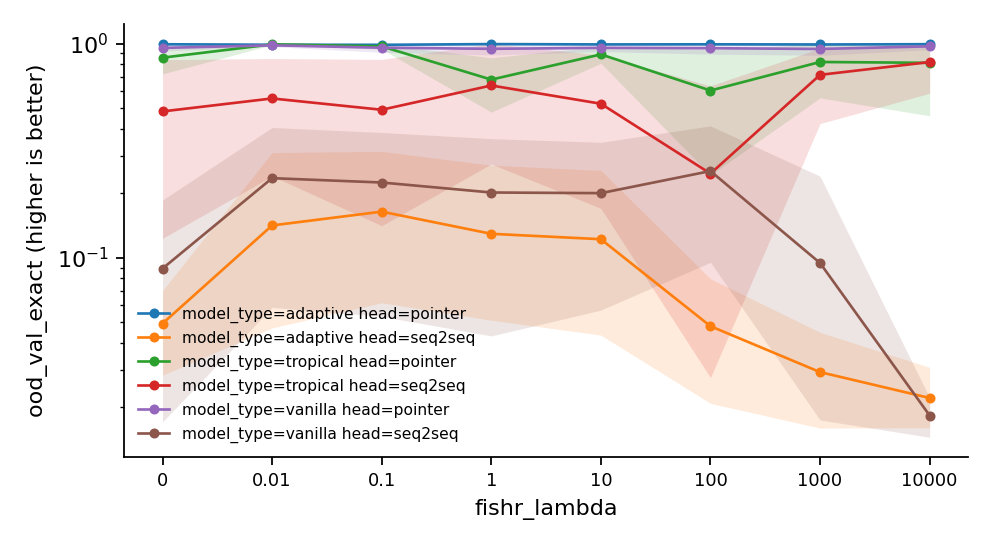
\includegraphics[width=\textwidth]{metric_ood_val_exact.png}
\caption{\texttt{ood\_val\_exact} against \texttt{fishr\_lambda}: the mean over seeds with a 95\% bootstrap CI, one line per combination of the other factors.}
\label{fig:ood_val_exact}
\end{figure}

{\small
\begin{longtable}{lllrlrrr}
\caption{\texttt{ood\_val\_exact} per cell: mean, 95\% bootstrap CI, SD, seeds, diverged runs.}\label{tab:summary-ood_val_exact}\\
\toprule
\texttt{model\_type} & \texttt{head} & \texttt{fishr\_lambda} & mean & 95\% CI & SD & $n$ & div.\\
\midrule
\endhead
adaptive & pointer & 0 & 0.9939 & [0.984, 1] & 0.011 & 5 & 0\\
adaptive & pointer & 0.01 & 0.9886 & [0.978, 0.998] & 0.0128 & 5 & 0\\
adaptive & pointer & 0.1 & 0.9879 & [0.972, 0.998] & 0.0172 & 5 & 0\\
adaptive & pointer & 1 & 0.9957 & [0.993, 0.998] & 0.00362 & 5 & 0\\
adaptive & pointer & 10 & 0.9921 & [0.987, 0.998] & 0.00713 & 5 & 0\\
adaptive & pointer & 100 & 0.9933 & [0.988, 0.999] & 0.0069 & 5 & 0\\
adaptive & pointer & 1000 & 0.9915 & [0.985, 0.997] & 0.00795 & 5 & 0\\
adaptive & pointer & 1e+04 & 0.9945 & [0.99, 1] & 0.00667 & 5 & 0\\
adaptive & seq2seq & 0 & 0.04928 & [0.0283, 0.0703] & 0.0268 & 5 & 0\\
adaptive & seq2seq & 0.01 & 0.1415 & [0.047, 0.31] & 0.187 & 5 & 0\\
adaptive & seq2seq & 0.1 & 0.1642 & [0.0616, 0.314] & 0.168 & 5 & 0\\
adaptive & seq2seq & 1 & 0.1294 & [0.0511, 0.271] & 0.157 & 5 & 0\\
adaptive & seq2seq & 10 & 0.1221 & [0.0435, 0.256] & 0.149 & 5 & 0\\
adaptive & seq2seq & 100 & 0.04788 & [0.0209, 0.0798] & 0.0376 & 5 & 0\\
adaptive & seq2seq & 1000 & 0.02922 & [0.016, 0.0448] & 0.0188 & 5 & 0\\
adaptive & seq2seq & 1e+04 & 0.02212 & [0.0161, 0.0307] & 0.00996 & 5 & 0\\
tropical & pointer & 0 & 0.8602 & [0.723, 0.972] & 0.161 & 5 & 0\\
tropical & pointer & 0.01 & 0.9929 & [0.988, 0.998] & 0.00701 & 5 & 0\\
tropical & pointer & 0.1 & 0.9715 & [0.942, 0.997] & 0.0345 & 5 & 0\\
tropical & pointer & 1 & 0.6795 & [0.479, 0.859] & 0.256 & 5 & 0\\
tropical & pointer & 10 & 0.8913 & [0.81, 0.972] & 0.104 & 5 & 0\\
tropical & pointer & 100 & 0.6042 & [0.243, 0.939] & 0.458 & 5 & 0\\
tropical & pointer & 1000 & 0.8212 & [0.558, 0.997] & 0.312 & 5 & 0\\
tropical & pointer & 1e+04 & 0.8138 & [0.46, 0.996] & 0.395 & 5 & 0\\
tropical & seq2seq & 0 & 0.4825 & [0.123, 0.842] & 0.478 & 5 & 0\\
tropical & seq2seq & 0.01 & 0.5548 & [0.241, 0.853] & 0.402 & 5 & 0\\
tropical & seq2seq & 0.1 & 0.4912 & [0.141, 0.844] & 0.471 & 5 & 0\\
tropical & seq2seq & 1 & 0.6379 & [0.274, 1] & 0.496 & 5 & 0\\
tropical & seq2seq & 10 & 0.5242 & [0.17, 0.885] & 0.455 & 5 & 0\\
tropical & seq2seq & 100 & 0.2472 & [0.0275, 0.635] & 0.424 & 5 & 0\\
tropical & seq2seq & 1000 & 0.7152 & [0.423, 0.952] & 0.348 & 5 & 0\\
tropical & seq2seq & 1e+04 & 0.8206 & [0.587, 1] & 0.264 & 5 & 0\\
vanilla & pointer & 0 & 0.9556 & [0.926, 0.987] & 0.0396 & 5 & 0\\
vanilla & pointer & 0.01 & 0.9825 & [0.968, 0.997] & 0.0189 & 5 & 0\\
vanilla & pointer & 0.1 & 0.9574 & [0.911, 0.999] & 0.0638 & 5 & 0\\
vanilla & pointer & 1 & 0.9464 & [0.886, 0.997] & 0.0801 & 5 & 0\\
vanilla & pointer & 10 & 0.9559 & [0.918, 0.993] & 0.0494 & 5 & 0\\
vanilla & pointer & 100 & 0.9526 & [0.893, 0.998] & 0.067 & 5 & 0\\
vanilla & pointer & 1000 & 0.9447 & [0.883, 0.993] & 0.0709 & 5 & 0\\
vanilla & pointer & 1e+04 & 0.9718 & [0.938, 0.996] & 0.0383 & 5 & 0\\
vanilla & seq2seq & 0 & 0.08902 & [0.0171, 0.186] & 0.108 & 5 & 0\\
vanilla & seq2seq & 0.01 & 0.2354 & [0.0586, 0.406] & 0.222 & 5 & 0\\
vanilla & seq2seq & 0.1 & 0.2246 & [0.0532, 0.385] & 0.216 & 5 & 0\\
vanilla & seq2seq & 1 & 0.2017 & [0.0431, 0.36] & 0.202 & 5 & 0\\
vanilla & seq2seq & 10 & 0.2003 & [0.0569, 0.346] & 0.187 & 5 & 0\\
vanilla & seq2seq & 100 & 0.2541 & [0.0952, 0.413] & 0.212 & 5 & 0\\
vanilla & seq2seq & 1000 & 0.09448 & [0.0175, 0.24] & 0.162 & 5 & 0\\
vanilla & seq2seq & 1e+04 & 0.01832 & [0.0145, 0.0222] & 0.00499 & 5 & 0\\
\bottomrule
\end{longtable}
}

{\small
\begin{longtable}{lllrrrl}
\caption{\texttt{ood\_val\_exact}: each level of \texttt{fishr\_lambda} against its control (0), within each combination of the other factors. rank: Wilcoxon signed-rank by seed, Holm.}\label{tab:control-ood_val_exact}\\
\toprule
\texttt{model\_type} & \texttt{head} & \texttt{fishr\_lambda} & difference & 95\% CI & $p$ & \\
\midrule
\endhead
adaptive & pointer & 0.01 & -0.0011 & [-0.0175, 0.00418] & 1.0000 & \\
adaptive & pointer & 0.1 & -0.0023 & [-0.0243, 0.00756] & 1.0000 & \\
adaptive & pointer & 1 & $-7.000\times10^{-4}$ & [-0.00418, 0.0092] & 1.0000 & \\
adaptive & pointer & 10 & $-4.000\times10^{-4}$ & [-0.00832, 0.0048] & 1.0000 & \\
adaptive & pointer & 100 & $-6.000\times10^{-4}$ & [-0.00724, 0.00602] & 1.0000 & \\
adaptive & pointer & 1000 & -0.0029 & [-0.011, 0.00586] & 1.0000 & \\
adaptive & pointer & 1e+04 & 0 & [-0.00688, 0.00766] & 1.0000 & \\
adaptive & seq2seq & 0.01 & 0.0328 & [-0.00556, 0.249] & 1.0000 & \\
adaptive & seq2seq & 0.1 & 0.0496 & [0.00608, 0.247] & 1.0000 & \\
adaptive & seq2seq & 1 & 0.0332 & [$3.78\times10^{-4}$, 0.208] & 1.0000 & \\
adaptive & seq2seq & 10 & 0.0211 & [-0.00341, 0.192] & 1.0000 & \\
adaptive & seq2seq & 100 & 0.0019 & [-0.0404, 0.0409] & 1.0000 & \\
adaptive & seq2seq & 1000 & -0.0132 & [-0.0437, -0.00482] & 0.4375 & \\
adaptive & seq2seq & 1e+04 & -0.0282 & [-0.0527, $3.60\times10^{-4}$] & 1.0000 & \\
tropical & pointer & 0.01 & 0.1048 & [0.021, 0.267] & 0.8750 & \\
tropical & pointer & 0.1 & 0.1035 & [0.0238, 0.227] & 0.8750 & \\
tropical & pointer & 1 & -0.1558 & [-0.375, 0.0209] & 1.0000 & \\
tropical & pointer & 10 & 0.0717 & [-0.0761, 0.119] & 1.0000 & \\
tropical & pointer & 100 & -0.0836 & [-0.548, 0.0179] & 1.0000 & \\
tropical & pointer & 1000 & 0.1049 & [-0.386, 0.245] & 1.0000 & \\
tropical & pointer & 1e+04 & 0.1038 & [-0.482, 0.258] & 1.0000 & \\
tropical & seq2seq & 0.01 & 0 & [-0.0476, 0.245] & 1.0000 & \\
tropical & seq2seq & 0.1 & 0 & [-0.429, 0.481] & 1.0000 & \\
tropical & seq2seq & 1 & 0 & [-0.0819, 0.57] & 1.0000 & \\
tropical & seq2seq & 10 & 0 & [-0.488, 0.589] & 1.0000 & \\
tropical & seq2seq & 100 & -0.058 & [-0.611, -0.00876] & 1.0000 & \\
tropical & seq2seq & 1000 & 0 & [-0.12, 0.585] & 1.0000 & \\
tropical & seq2seq & 1e+04 & 0.2064 & [-0.0541, 0.76] & 1.0000 & \\
vanilla & pointer & 0.01 & 0.0348 & [-0.00312, 0.0569] & 1.0000 & \\
vanilla & pointer & 0.1 & 0.001 & [-0.0413, 0.0467] & 1.0000 & \\
vanilla & pointer & 1 & 0.001 & [-0.0625, 0.0445] & 1.0000 & \\
vanilla & pointer & 10 & $9.000\times10^{-4}$ & [-0.0435, 0.039] & 1.0000 & \\
vanilla & pointer & 100 & $9.000\times10^{-4}$ & [-0.0482, 0.046] & 1.0000 & \\
vanilla & pointer & 1000 & 0.0013 & [-0.0575, 0.0373] & 1.0000 & \\
vanilla & pointer & 1e+04 & 0.0013 & [-0.00774, 0.0465] & 1.0000 & \\
vanilla & seq2seq & 0.01 & 0.1779 & [-0.00382, 0.303] & 1.0000 & \\
vanilla & seq2seq & 0.1 & 0.157 & [-0.0132, 0.309] & 1.0000 & \\
vanilla & seq2seq & 1 & 0.1231 & [-0.0201, 0.262] & 1.0000 & \\
vanilla & seq2seq & 10 & 0.1663 & [-0.0202, 0.231] & 1.0000 & \\
vanilla & seq2seq & 100 & 0.1419 & [-0.0118, 0.342] & 1.0000 & \\
vanilla & seq2seq & 1000 & $2.000\times10^{-4}$ & [-0.0637, 0.0737] & 1.0000 & \\
vanilla & seq2seq & 1e+04 & -0.0026 & [-0.15, 0.0018] & 1.0000 & \\
\bottomrule
\end{longtable}
}

{\small
\begin{longtable}{llrrrrr}
\caption{\texttt{ood\_val\_exact} against log10 \texttt{fishr\_lambda}: rank: Spearman rho, seed-bootstrap CI, with the Jonckheere--Terpstra ordered-trend $\tau$ and $p$.}\label{tab:trend-ood_val_exact}\\
\toprule
\texttt{model\_type} & \texttt{head} & estimate & 95\% CI & $p$ & JT $\tau$ & JT $p$\\
\midrule
\endhead
adaptive & pointer & 0.1054 & [-0.0851, 0.343] & 0.5467 & 0.0724 & 0.6001\\
adaptive & seq2seq & -0.6344 & [-0.802, -0.407] & $<10^{-4}$ & -0.503 & 0.0004\\
tropical & pointer & -0.1782 & [-0.567, 0.116] & 0.3057 & -0.15 & 0.2629\\
tropical & seq2seq & 0.1162 & [-0.106, 0.321] & 0.5064 & 0.0705 & 0.5871\\
vanilla & pointer & -0.0573 & [-0.292, 0.207] & 0.7437 & -0.0533 & 0.6985\\
vanilla & seq2seq & -0.4025 & [-0.719, -0.197] & 0.0165 & -0.32 & 0.0170\\
\bottomrule
\end{longtable}
}

{\small
\begin{longtable}{lrrrl}
\caption{\texttt{ood\_val\_exact}: paired contrasts by seed, Holm-corrected across the cells. rank: Wilcoxon signed-rank by seed, Holm.}\label{tab:paired-ood_val_exact}\\
\toprule
contrast (within) & difference & 95\% CI & $p$ & \\
\midrule
\endhead
\stackcell{model\_type: tropical - vanilla\\\footnotesize head=pointer fishr\_lambda=0 } & -0.09536 & [-0.294, 0.104] & 1.0000 & \\
\stackcell{model\_type: tropical - vanilla\\\footnotesize head=pointer fishr\_lambda=0.01 } & 0.01038 & [-0.0168, 0.0375] & 1.0000 & \\
\stackcell{model\_type: tropical - vanilla\\\footnotesize head=pointer fishr\_lambda=0.1 } & 0.01412 & [-0.0501, 0.0784] & 1.0000 & \\
\stackcell{model\_type: tropical - vanilla\\\footnotesize head=pointer fishr\_lambda=1 } & -0.2669 & [-0.645, 0.112] & 1.0000 & \\
\stackcell{model\_type: tropical - vanilla\\\footnotesize head=pointer fishr\_lambda=10 } & -0.06462 & [-0.189, 0.0596] & 1.0000 & \\
\stackcell{model\_type: tropical - vanilla\\\footnotesize head=pointer fishr\_lambda=100 } & -0.3484 & [-0.972, 0.276] & 1.0000 & \\
\stackcell{model\_type: tropical - vanilla\\\footnotesize head=pointer fishr\_lambda=1000 } & -0.1235 & [-0.512, 0.265] & 1.0000 & \\
\stackcell{model\_type: tropical - vanilla\\\footnotesize head=pointer fishr\_lambda=1e+04 } & -0.158 & [-0.65, 0.334] & 1.0000 & \\
\stackcell{model\_type: tropical - vanilla\\\footnotesize head=seq2seq fishr\_lambda=0 } & 0.3935 & [-0.0833, 0.87] & 1.0000 & \\
\stackcell{model\_type: tropical - vanilla\\\footnotesize head=seq2seq fishr\_lambda=0.01 } & 0.3194 & [-0.267, 0.905] & 1.0000 & \\
\stackcell{model\_type: tropical - vanilla\\\footnotesize head=seq2seq fishr\_lambda=0.1 } & 0.2666 & [-0.108, 0.641] & 1.0000 & \\
\stackcell{model\_type: tropical - vanilla\\\footnotesize head=seq2seq fishr\_lambda=1 } & 0.4362 & [-0.303, 1.18] & 1.0000 & \\
\stackcell{model\_type: tropical - vanilla\\\footnotesize head=seq2seq fishr\_lambda=10 } & 0.3239 & [-0.224, 0.872] & 1.0000 & \\
\stackcell{model\_type: tropical - vanilla\\\footnotesize head=seq2seq fishr\_lambda=100 } & -0.00682 & [-0.473, 0.46] & 1.0000 & \\
\stackcell{model\_type: tropical - vanilla\\\footnotesize head=seq2seq fishr\_lambda=1000 } & 0.6207 & [0.228, 1.01] & 1.0000 & \\
\stackcell{model\_type: tropical - vanilla\\\footnotesize head=seq2seq fishr\_lambda=1e+04 } & 0.8022 & [0.475, 1.13] & 1.0000 & \\
\stackcell{model\_type: adaptive - vanilla\\\footnotesize head=pointer fishr\_lambda=0 } & 0.03828 & [-0.0197, 0.0962] & 1.0000 & \\
\stackcell{model\_type: adaptive - vanilla\\\footnotesize head=pointer fishr\_lambda=0.01 } & 0.00608 & [-0.00354, 0.0157] & 1.0000 & \\
\stackcell{model\_type: adaptive - vanilla\\\footnotesize head=pointer fishr\_lambda=0.1 } & 0.03052 & [-0.0279, 0.089] & 1.0000 & \\
\stackcell{model\_type: adaptive - vanilla\\\footnotesize head=pointer fishr\_lambda=1 } & 0.04928 & [-0.0507, 0.149] & 1.0000 & \\
\stackcell{model\_type: adaptive - vanilla\\\footnotesize head=pointer fishr\_lambda=10 } & 0.03618 & [-0.0195, 0.0918] & 1.0000 & \\
\stackcell{model\_type: adaptive - vanilla\\\footnotesize head=pointer fishr\_lambda=100 } & 0.04068 & [-0.035, 0.116] & 1.0000 & \\
\stackcell{model\_type: adaptive - vanilla\\\footnotesize head=pointer fishr\_lambda=1000 } & 0.04676 & [-0.0317, 0.125] & 1.0000 & \\
\stackcell{model\_type: adaptive - vanilla\\\footnotesize head=pointer fishr\_lambda=1e+04 } & 0.02272 & [-0.0263, 0.0717] & 1.0000 & \\
\stackcell{model\_type: adaptive - vanilla\\\footnotesize head=seq2seq fishr\_lambda=0 } & -0.03974 & [-0.147, 0.0673] & 1.0000 & \\
\stackcell{model\_type: adaptive - vanilla\\\footnotesize head=seq2seq fishr\_lambda=0.01 } & -0.09382 & [-0.302, 0.114] & 1.0000 & \\
\stackcell{model\_type: adaptive - vanilla\\\footnotesize head=seq2seq fishr\_lambda=0.1 } & -0.06042 & [-0.328, 0.207] & 1.0000 & \\
\stackcell{model\_type: adaptive - vanilla\\\footnotesize head=seq2seq fishr\_lambda=1 } & -0.07236 & [-0.271, 0.126] & 1.0000 & \\
\stackcell{model\_type: adaptive - vanilla\\\footnotesize head=seq2seq fishr\_lambda=10 } & -0.07826 & [-0.221, 0.0641] & 1.0000 & \\
\stackcell{model\_type: adaptive - vanilla\\\footnotesize head=seq2seq fishr\_lambda=100 } & -0.2062 & [-0.448, 0.0357] & 1.0000 & \\
\stackcell{model\_type: adaptive - vanilla\\\footnotesize head=seq2seq fishr\_lambda=1000 } & -0.06526 & [-0.279, 0.148] & 1.0000 & \\
\stackcell{model\_type: adaptive - vanilla\\\footnotesize head=seq2seq fishr\_lambda=1e+04 } & 0.0038 & [-0.0116, 0.0192] & 1.0000 & \\
\stackcell{head: pointer - seq2seq\\\footnotesize model\_type=adaptive fishr\_lambda=0 } & 0.9446 & [0.901, 0.988] & 1.0000 & \\
\stackcell{head: pointer - seq2seq\\\footnotesize model\_type=adaptive fishr\_lambda=0.01 } & 0.847 & [0.612, 1.08] & 1.0000 & \\
\stackcell{head: pointer - seq2seq\\\footnotesize model\_type=adaptive fishr\_lambda=0.1 } & 0.8237 & [0.618, 1.03] & 1.0000 & \\
\stackcell{head: pointer - seq2seq\\\footnotesize model\_type=adaptive fishr\_lambda=1 } & 0.8663 & [0.668, 1.06] & 1.0000 & \\
\stackcell{head: pointer - seq2seq\\\footnotesize model\_type=adaptive fishr\_lambda=10 } & 0.8701 & [0.68, 1.06] & 1.0000 & \\
\stackcell{head: pointer - seq2seq\\\footnotesize model\_type=adaptive fishr\_lambda=100 } & 0.9454 & [0.904, 0.987] & 1.0000 & \\
\stackcell{head: pointer - seq2seq\\\footnotesize model\_type=adaptive fishr\_lambda=1000 } & 0.9623 & [0.933, 0.991] & 1.0000 & \\
\stackcell{head: pointer - seq2seq\\\footnotesize model\_type=adaptive fishr\_lambda=1e+04 } & 0.9724 & [0.955, 0.99] & 1.0000 & \\
\stackcell{head: pointer - seq2seq\\\footnotesize model\_type=tropical fishr\_lambda=0 } & 0.3778 & [-0.166, 0.922] & 1.0000 & \\
\stackcell{head: pointer - seq2seq\\\footnotesize model\_type=tropical fishr\_lambda=0.01 } & 0.4381 & [-0.0587, 0.935] & 1.0000 & \\
\stackcell{head: pointer - seq2seq\\\footnotesize model\_type=tropical fishr\_lambda=0.1 } & 0.4803 & [-0.0805, 1.04] & 1.0000 & \\
\stackcell{head: pointer - seq2seq\\\footnotesize model\_type=tropical fishr\_lambda=1 } & 0.04158 & [-0.75, 0.833] & 1.0000 & \\
\stackcell{head: pointer - seq2seq\\\footnotesize model\_type=tropical fishr\_lambda=10 } & 0.3671 & [-0.304, 1.04] & 1.0000 & \\
\stackcell{head: pointer - seq2seq\\\footnotesize model\_type=tropical fishr\_lambda=100 } & 0.3569 & [-0.278, 0.992] & 1.0000 & \\
\stackcell{head: pointer - seq2seq\\\footnotesize model\_type=tropical fishr\_lambda=1000 } & 0.106 & [-0.622, 0.834] & 1.0000 & \\
\stackcell{head: pointer - seq2seq\\\footnotesize model\_type=tropical fishr\_lambda=1e+04 } & -0.00672 & [-0.694, 0.681] & 1.0000 & \\
\stackcell{head: pointer - seq2seq\\\footnotesize model\_type=vanilla fishr\_lambda=0 } & 0.8666 & [0.732, 1] & 1.0000 & \\
\stackcell{head: pointer - seq2seq\\\footnotesize model\_type=vanilla fishr\_lambda=0.01 } & 0.7471 & [0.471, 1.02] & 1.0000 & \\
\stackcell{head: pointer - seq2seq\\\footnotesize model\_type=vanilla fishr\_lambda=0.1 } & 0.7328 & [0.48, 0.985] & 1.0000 & \\
\stackcell{head: pointer - seq2seq\\\footnotesize model\_type=vanilla fishr\_lambda=1 } & 0.7447 & [0.504, 0.985] & 1.0000 & \\
\stackcell{head: pointer - seq2seq\\\footnotesize model\_type=vanilla fishr\_lambda=10 } & 0.7556 & [0.51, 1] & 1.0000 & \\
\stackcell{head: pointer - seq2seq\\\footnotesize model\_type=vanilla fishr\_lambda=100 } & 0.6985 & [0.456, 0.942] & 1.0000 & \\
\stackcell{head: pointer - seq2seq\\\footnotesize model\_type=vanilla fishr\_lambda=1000 } & 0.8502 & [0.616, 1.08] & 1.0000 & \\
\stackcell{head: pointer - seq2seq\\\footnotesize model\_type=vanilla fishr\_lambda=1e+04 } & 0.9535 & [0.904, 1] & 1.0000 & \\
\bottomrule
\end{longtable}
}

\subsection{\texttt{ood\_noise\_f1}}
\begin{figure}[tbp]
\centering
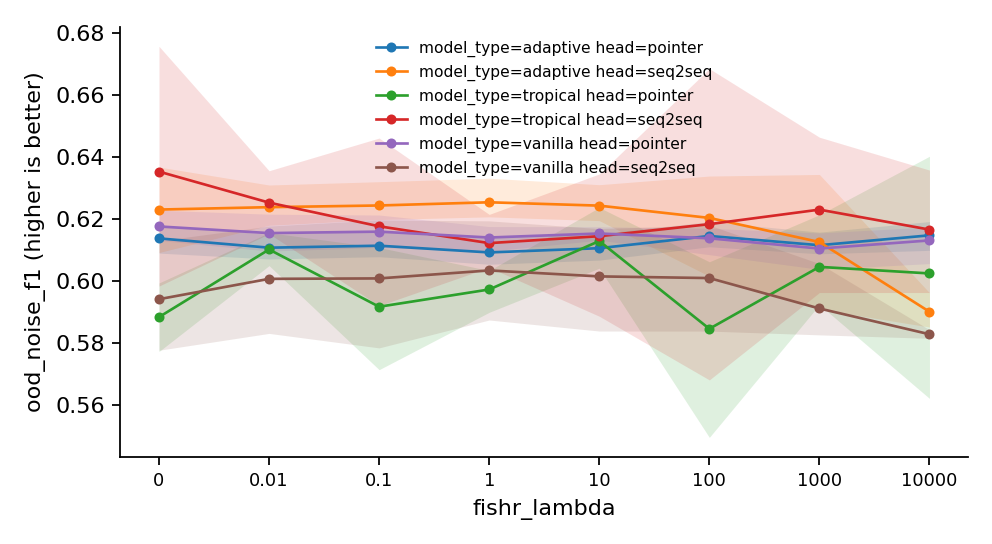
\includegraphics[width=\textwidth]{metric_ood_noise_f1.png}
\caption{\texttt{ood\_noise\_f1} against \texttt{fishr\_lambda}: the mean over seeds with a 95\% bootstrap CI, one line per combination of the other factors.}
\label{fig:ood_noise_f1}
\end{figure}

{\small
\begin{longtable}{lllrlrrr}
\caption{\texttt{ood\_noise\_f1} per cell: mean, 95\% bootstrap CI, SD, seeds, diverged runs.}\label{tab:summary-ood_noise_f1}\\
\toprule
\texttt{model\_type} & \texttt{head} & \texttt{fishr\_lambda} & mean & 95\% CI & SD & $n$ & div.\\
\midrule
\endhead
adaptive & pointer & 0 & 0.6138 & [0.609, 0.618] & 0.00555 & 5 & 0\\
adaptive & pointer & 0.01 & 0.6108 & [0.607, 0.615] & 0.0051 & 5 & 0\\
adaptive & pointer & 0.1 & 0.6114 & [0.608, 0.616] & 0.00525 & 5 & 0\\
adaptive & pointer & 1 & 0.6092 & [0.605, 0.614] & 0.00588 & 5 & 0\\
adaptive & pointer & 10 & 0.6106 & [0.607, 0.615] & 0.00553 & 5 & 0\\
adaptive & pointer & 100 & 0.6145 & [0.611, 0.619] & 0.00534 & 5 & 0\\
adaptive & pointer & 1000 & 0.6116 & [0.609, 0.616] & 0.0046 & 5 & 0\\
adaptive & pointer & 1e+04 & 0.6147 & [0.61, 0.619] & 0.00597 & 5 & 0\\
adaptive & seq2seq & 0 & 0.6231 & [0.609, 0.637] & 0.0168 & 5 & 0\\
adaptive & seq2seq & 0.01 & 0.6238 & [0.618, 0.631] & 0.00813 & 5 & 0\\
adaptive & seq2seq & 0.1 & 0.6244 & [0.62, 0.632] & 0.00851 & 5 & 0\\
adaptive & seq2seq & 1 & 0.6254 & [0.621, 0.633] & 0.00855 & 5 & 0\\
adaptive & seq2seq & 10 & 0.6243 & [0.619, 0.631] & 0.0079 & 5 & 0\\
adaptive & seq2seq & 100 & 0.6204 & [0.602, 0.634] & 0.0213 & 5 & 0\\
adaptive & seq2seq & 1000 & 0.6126 & [0.591, 0.634] & 0.0287 & 5 & 0\\
adaptive & seq2seq & 1e+04 & 0.5901 & [0.585, 0.596] & 0.0075 & 5 & 0\\
tropical & pointer & 0 & 0.5884 & [0.577, 0.599] & 0.0144 & 5 & 0\\
tropical & pointer & 0.01 & 0.6102 & [0.605, 0.616] & 0.00691 & 5 & 0\\
tropical & pointer & 0.1 & 0.5917 & [0.571, 0.611] & 0.0272 & 5 & 0\\
tropical & pointer & 1 & 0.5973 & [0.59, 0.603] & 0.0087 & 5 & 0\\
tropical & pointer & 10 & 0.6129 & [0.604, 0.624] & 0.0128 & 5 & 0\\
tropical & pointer & 100 & 0.5846 & [0.55, 0.606] & 0.0394 & 5 & 0\\
tropical & pointer & 1000 & 0.6046 & [0.592, 0.621] & 0.0187 & 5 & 0\\
tropical & pointer & 1e+04 & 0.6025 & [0.562, 0.64] & 0.0466 & 5 & 0\\
tropical & seq2seq & 0 & 0.6353 & [0.598, 0.676] & 0.0494 & 5 & 0\\
tropical & seq2seq & 0.01 & 0.6253 & [0.615, 0.636] & 0.0133 & 5 & 0\\
tropical & seq2seq & 0.1 & 0.6177 & [0.592, 0.646] & 0.036 & 5 & 0\\
tropical & seq2seq & 1 & 0.6122 & [0.604, 0.621] & 0.0109 & 5 & 0\\
tropical & seq2seq & 10 & 0.6145 & [0.589, 0.635] & 0.0308 & 5 & 0\\
tropical & seq2seq & 100 & 0.6184 & [0.568, 0.668] & 0.0634 & 5 & 0\\
tropical & seq2seq & 1000 & 0.623 & [0.596, 0.646] & 0.0327 & 5 & 0\\
tropical & seq2seq & 1e+04 & 0.6166 & [0.596, 0.636] & 0.0264 & 5 & 0\\
vanilla & pointer & 0 & 0.6176 & [0.613, 0.623] & 0.00585 & 5 & 0\\
vanilla & pointer & 0.01 & 0.6155 & [0.61, 0.622] & 0.00728 & 5 & 0\\
vanilla & pointer & 0.1 & 0.6159 & [0.611, 0.621] & 0.00643 & 5 & 0\\
vanilla & pointer & 1 & 0.614 & [0.61, 0.618] & 0.00505 & 5 & 0\\
vanilla & pointer & 10 & 0.6153 & [0.613, 0.618] & 0.00276 & 5 & 0\\
vanilla & pointer & 100 & 0.6138 & [0.609, 0.617] & 0.00597 & 5 & 0\\
vanilla & pointer & 1000 & 0.6105 & [0.604, 0.616] & 0.00789 & 5 & 0\\
vanilla & pointer & 1e+04 & 0.6131 & [0.606, 0.617] & 0.00809 & 5 & 0\\
vanilla & seq2seq & 0 & 0.5942 & [0.578, 0.613] & 0.0226 & 5 & 0\\
vanilla & seq2seq & 0.01 & 0.6007 & [0.583, 0.618] & 0.0224 & 5 & 0\\
vanilla & seq2seq & 0.1 & 0.6009 & [0.578, 0.62] & 0.0266 & 5 & 0\\
vanilla & seq2seq & 1 & 0.6034 & [0.587, 0.619] & 0.0212 & 5 & 0\\
vanilla & seq2seq & 10 & 0.6015 & [0.584, 0.617] & 0.0216 & 5 & 0\\
vanilla & seq2seq & 100 & 0.601 & [0.584, 0.618] & 0.023 & 5 & 0\\
vanilla & seq2seq & 1000 & 0.5912 & [0.583, 0.606] & 0.0159 & 5 & 0\\
vanilla & seq2seq & 1e+04 & 0.5829 & [0.582, 0.584] & 0.0019 & 5 & 0\\
\bottomrule
\end{longtable}
}

{\small
\begin{longtable}{lllrrrl}
\caption{\texttt{ood\_noise\_f1}: each level of \texttt{fishr\_lambda} against its control (0), within each combination of the other factors. parametric: Dunnett vs control.}\label{tab:control-ood_noise_f1}\\
\toprule
\texttt{model\_type} & \texttt{head} & \texttt{fishr\_lambda} & difference & 95\% CI & $p$ & \\
\midrule
\endhead
adaptive & pointer & 0.01 & -0.002997 & [-0.0125, 0.00647] & 0.9155 & \\
adaptive & pointer & 0.1 & -0.00236 & [-0.0118, 0.00711] & 0.9727 & \\
adaptive & pointer & 1 & -0.004524 & [-0.014, 0.00494] & 0.6446 & \\
adaptive & pointer & 10 & -0.003162 & [-0.0126, 0.0063] & 0.8941 & \\
adaptive & pointer & 100 & $7.766\times10^{-4}$ & [-0.00869, 0.0102] & 1.0000 & \\
adaptive & pointer & 1000 & -0.002202 & [-0.0117, 0.00726] & 0.9810 & \\
adaptive & pointer & 1e+04 & $9.809\times10^{-4}$ & [-0.00849, 0.0104] & 0.9999 & \\
adaptive & seq2seq & 0.01 & $7.714\times10^{-4}$ & [-0.0261, 0.0276] & 1.0000 & \\
adaptive & seq2seq & 0.1 & 0.001316 & [-0.0255, 0.0282] & 1.0000 & \\
adaptive & seq2seq & 1 & 0.002343 & [-0.0245, 0.0292] & 1.0000 & \\
adaptive & seq2seq & 10 & 0.001266 & [-0.0256, 0.0281] & 1.0000 & \\
adaptive & seq2seq & 100 & -0.002697 & [-0.0295, 0.0241] & 0.9999 & \\
adaptive & seq2seq & 1000 & -0.01047 & [-0.0373, 0.0164] & 0.8091 & \\
adaptive & seq2seq & 1e+04 & -0.03295 & [-0.0598, -0.0061] & 0.0110 & *\\
tropical & pointer & 0.01 & 0.0218 & [-0.0232, 0.0668] & 0.6323 & \\
tropical & pointer & 0.1 & 0.003337 & [-0.0417, 0.0484] & 1.0000 & \\
tropical & pointer & 1 & 0.008903 & [-0.0361, 0.0539] & 0.9923 & \\
tropical & pointer & 10 & 0.02453 & [-0.0205, 0.0696] & 0.5152 & \\
tropical & pointer & 100 & -0.003776 & [-0.0488, 0.0413] & 1.0000 & \\
tropical & pointer & 1000 & 0.01619 & [-0.0288, 0.0612] & 0.8582 & \\
tropical & pointer & 1e+04 & 0.01408 & [-0.031, 0.0591] & 0.9200 & \\
tropical & seq2seq & 0.01 & -0.01 & [-0.0741, 0.0541] & 0.9981 & \\
tropical & seq2seq & 0.1 & -0.01764 & [-0.0817, 0.0464] & 0.9554 & \\
tropical & seq2seq & 1 & -0.02306 & [-0.0871, 0.041] & 0.8579 & \\
tropical & seq2seq & 10 & -0.02083 & [-0.0849, 0.0433] & 0.9055 & \\
tropical & seq2seq & 100 & -0.01694 & [-0.081, 0.0471] & 0.9633 & \\
tropical & seq2seq & 1000 & -0.01226 & [-0.0763, 0.0518] & 0.9936 & \\
tropical & seq2seq & 1e+04 & -0.0187 & [-0.0828, 0.0454] & 0.9413 & \\
vanilla & pointer & 0.01 & -0.002141 & [-0.0133, 0.00899] & 0.9934 & \\
vanilla & pointer & 0.1 & -0.00167 & [-0.0128, 0.00946] & 0.9985 & \\
vanilla & pointer & 1 & -0.003564 & [-0.0147, 0.00757] & 0.9114 & \\
vanilla & pointer & 10 & -0.00227 & [-0.0134, 0.00887] & 0.9908 & \\
vanilla & pointer & 100 & -0.003817 & [-0.015, 0.00732] & 0.8823 & \\
vanilla & pointer & 1000 & -0.007122 & [-0.0183, 0.00401] & 0.3516 & \\
vanilla & pointer & 1e+04 & -0.004503 & [-0.0156, 0.00663] & 0.7843 & \\
vanilla & seq2seq & 0.01 & 0.006557 & [-0.0296, 0.0427] & 0.9953 & \\
vanilla & seq2seq & 0.1 & 0.006698 & [-0.0294, 0.0428] & 0.9947 & \\
vanilla & seq2seq & 1 & 0.00927 & [-0.0269, 0.0454] & 0.9684 & \\
vanilla & seq2seq & 10 & 0.007349 & [-0.0288, 0.0435] & 0.9909 & \\
vanilla & seq2seq & 100 & 0.006808 & [-0.0293, 0.0429] & 0.9941 & \\
vanilla & seq2seq & 1000 & -0.003001 & [-0.0391, 0.0331] & 1.0000 & \\
vanilla & seq2seq & 1e+04 & -0.0113 & [-0.0474, 0.0248] & 0.9198 & \\
\bottomrule
\end{longtable}
}

{\small
\begin{longtable}{llrrrrr}
\caption{\texttt{ood\_noise\_f1} against log10 \texttt{fishr\_lambda}: parametric: OLS slope t-test, seed-bootstrap CI, with the Jonckheere--Terpstra ordered-trend $\tau$ and $p$.}\label{tab:trend-ood_noise_f1}\\
\toprule
\texttt{model\_type} & \texttt{head} & estimate & 95\% CI & $p$ & JT $\tau$ & JT $p$\\
\midrule
\endhead
adaptive & pointer & $6.267\times10^{-4}$ & [$3.61\times10^{-4}$, 0.00108] & 0.1624 & 0.189 & 0.1564\\
adaptive & seq2seq & -0.004635 & [-0.0058, -0.00347] & 0.0015 & -0.208 & 0.1254\\
tropical & pointer & $-3.622\times10^{-4}$ & [-0.00387, 0.00385] & 0.8733 & -0.0667 & 0.6331\\
tropical & seq2seq & $-3.291\times10^{-4}$ & [-0.0038, 0.0033] & 0.9041 & 0.0019 & 1.0000\\
vanilla & pointer & $-6.515\times10^{-4}$ & [-0.00146, $8.11\times10^{-5}$] & 0.2116 & -0.0438 & 0.7415\\
vanilla & seq2seq & -0.002694 & [-0.00571, $3.23\times10^{-4}$] & 0.1085 & -0.2 & 0.1274\\
\bottomrule
\end{longtable}
}

{\small
\begin{longtable}{lrrrl}
\caption{\texttt{ood\_noise\_f1}: paired contrasts by seed, Holm-corrected across the cells. parametric: paired t-test by seed, Holm.}\label{tab:paired-ood_noise_f1}\\
\toprule
contrast (within) & difference & 95\% CI & $p$ & \\
\midrule
\endhead
\stackcell{model\_type: tropical - vanilla\\\footnotesize head=pointer fishr\_lambda=0 } & -0.02922 & [-0.0429, -0.0156] & 0.0641 & \\
\stackcell{model\_type: tropical - vanilla\\\footnotesize head=pointer fishr\_lambda=0.01 } & -0.005279 & [-0.014, 0.00341] & 1.0000 & \\
\stackcell{model\_type: tropical - vanilla\\\footnotesize head=pointer fishr\_lambda=0.1 } & -0.02421 & [-0.0619, 0.0134] & 1.0000 & \\
\stackcell{model\_type: tropical - vanilla\\\footnotesize head=pointer fishr\_lambda=1 } & -0.01675 & [-0.0288, -0.00472] & 0.2708 & \\
\stackcell{model\_type: tropical - vanilla\\\footnotesize head=pointer fishr\_lambda=10 } & -0.002425 & [-0.0187, 0.0139] & 1.0000 & \\
\stackcell{model\_type: tropical - vanilla\\\footnotesize head=pointer fishr\_lambda=100 } & -0.02918 & [-0.0809, 0.0226] & 1.0000 & \\
\stackcell{model\_type: tropical - vanilla\\\footnotesize head=pointer fishr\_lambda=1000 } & -0.005907 & [-0.0343, 0.0225] & 1.0000 & \\
\stackcell{model\_type: tropical - vanilla\\\footnotesize head=pointer fishr\_lambda=1e+04 } & -0.01064 & [-0.0764, 0.0551] & 1.0000 & \\
\stackcell{model\_type: tropical - vanilla\\\footnotesize head=seq2seq fishr\_lambda=0 } & 0.04113 & [-0.0149, 0.0972] & 1.0000 & \\
\stackcell{model\_type: tropical - vanilla\\\footnotesize head=seq2seq fishr\_lambda=0.01 } & 0.02458 & [-0.00249, 0.0516] & 0.7831 & \\
\stackcell{model\_type: tropical - vanilla\\\footnotesize head=seq2seq fishr\_lambda=0.1 } & 0.0168 & [-0.0272, 0.0608] & 1.0000 & \\
\stackcell{model\_type: tropical - vanilla\\\footnotesize head=seq2seq fishr\_lambda=1 } & 0.008809 & [-0.0268, 0.0445] & 1.0000 & \\
\stackcell{model\_type: tropical - vanilla\\\footnotesize head=seq2seq fishr\_lambda=10 } & 0.01296 & [-0.0342, 0.0601] & 1.0000 & \\
\stackcell{model\_type: tropical - vanilla\\\footnotesize head=seq2seq fishr\_lambda=100 } & 0.01738 & [-0.0427, 0.0775] & 1.0000 & \\
\stackcell{model\_type: tropical - vanilla\\\footnotesize head=seq2seq fishr\_lambda=1000 } & 0.03188 & [0.00463, 0.0591] & 0.4398 & \\
\stackcell{model\_type: tropical - vanilla\\\footnotesize head=seq2seq fishr\_lambda=1e+04 } & 0.03374 & [$1.58\times10^{-4}$, 0.0673] & 0.6414 & \\
\stackcell{model\_type: adaptive - vanilla\\\footnotesize head=pointer fishr\_lambda=0 } & -0.003846 & [-0.00642, -0.00127] & 0.2002 & \\
\stackcell{model\_type: adaptive - vanilla\\\footnotesize head=pointer fishr\_lambda=0.01 } & -0.004702 & [-0.00966, $2.53\times10^{-4}$] & 0.7526 & \\
\stackcell{model\_type: adaptive - vanilla\\\footnotesize head=pointer fishr\_lambda=0.1 } & -0.004536 & [-0.00706, -0.00201] & 0.1211 & \\
\stackcell{model\_type: adaptive - vanilla\\\footnotesize head=pointer fishr\_lambda=1 } & -0.004806 & [-0.0103, $6.63\times10^{-4}$] & 0.8546 & \\
\stackcell{model\_type: adaptive - vanilla\\\footnotesize head=pointer fishr\_lambda=10 } & -0.004739 & [-0.0103, $8.27\times10^{-4}$] & 0.8546 & \\
\stackcell{model\_type: adaptive - vanilla\\\footnotesize head=pointer fishr\_lambda=100 } & $7.479\times10^{-4}$ & [-0.00566, 0.00716] & 1.0000 & \\
\stackcell{model\_type: adaptive - vanilla\\\footnotesize head=pointer fishr\_lambda=1000 } & 0.001074 & [-0.00963, 0.0118] & 1.0000 & \\
\stackcell{model\_type: adaptive - vanilla\\\footnotesize head=pointer fishr\_lambda=1e+04 } & 0.001637 & [-0.00468, 0.00795] & 1.0000 & \\
\stackcell{model\_type: adaptive - vanilla\\\footnotesize head=seq2seq fishr\_lambda=0 } & 0.0289 & [0.011, 0.0468] & 0.1650 & \\
\stackcell{model\_type: adaptive - vanilla\\\footnotesize head=seq2seq fishr\_lambda=0.01 } & 0.02311 & [-0.00985, 0.0561] & 1.0000 & \\
\stackcell{model\_type: adaptive - vanilla\\\footnotesize head=seq2seq fishr\_lambda=0.1 } & 0.02352 & [-0.0189, 0.0659] & 1.0000 & \\
\stackcell{model\_type: adaptive - vanilla\\\footnotesize head=seq2seq fishr\_lambda=1 } & 0.02197 & [-0.0132, 0.0572] & 1.0000 & \\
\stackcell{model\_type: adaptive - vanilla\\\footnotesize head=seq2seq fishr\_lambda=10 } & 0.02281 & [-0.0115, 0.0572] & 1.0000 & \\
\stackcell{model\_type: adaptive - vanilla\\\footnotesize head=seq2seq fishr\_lambda=100 } & 0.01939 & [-0.0124, 0.0512] & 1.0000 & \\
\stackcell{model\_type: adaptive - vanilla\\\footnotesize head=seq2seq fishr\_lambda=1000 } & 0.02143 & [-0.0278, 0.0706] & 1.0000 & \\
\stackcell{model\_type: adaptive - vanilla\\\footnotesize head=seq2seq fishr\_lambda=1e+04 } & 0.007251 & [-0.0029, 0.0174] & 1.0000 & \\
\stackcell{head: pointer - seq2seq\\\footnotesize model\_type=adaptive fishr\_lambda=0 } & -0.009295 & [-0.0311, 0.0125] & 1.0000 & \\
\stackcell{head: pointer - seq2seq\\\footnotesize model\_type=adaptive fishr\_lambda=0.01 } & -0.01306 & [-0.0277, 0.0016] & 1.0000 & \\
\stackcell{head: pointer - seq2seq\\\footnotesize model\_type=adaptive fishr\_lambda=0.1 } & -0.01297 & [-0.0262, $2.89\times10^{-4}$] & 1.0000 & \\
\stackcell{head: pointer - seq2seq\\\footnotesize model\_type=adaptive fishr\_lambda=1 } & -0.01616 & [-0.031, -0.00136] & 0.8521 & \\
\stackcell{head: pointer - seq2seq\\\footnotesize model\_type=adaptive fishr\_lambda=10 } & -0.01372 & [-0.0275, $8.65\times10^{-5}$] & 1.0000 & \\
\stackcell{head: pointer - seq2seq\\\footnotesize model\_type=adaptive fishr\_lambda=100 } & -0.005821 & [-0.0386, 0.0269] & 1.0000 & \\
\stackcell{head: pointer - seq2seq\\\footnotesize model\_type=adaptive fishr\_lambda=1000 } & -0.001025 & [-0.0411, 0.039] & 1.0000 & \\
\stackcell{head: pointer - seq2seq\\\footnotesize model\_type=adaptive fishr\_lambda=1e+04 } & 0.02463 & [0.0185, 0.0307] & 0.0086 & *\\
\stackcell{head: pointer - seq2seq\\\footnotesize model\_type=tropical fishr\_lambda=0 } & -0.04691 & [-0.108, 0.0138] & 1.0000 & \\
\stackcell{head: pointer - seq2seq\\\footnotesize model\_type=tropical fishr\_lambda=0.01 } & -0.01511 & [-0.032, 0.00176] & 1.0000 & \\
\stackcell{head: pointer - seq2seq\\\footnotesize model\_type=tropical fishr\_lambda=0.1 } & -0.02593 & [-0.0843, 0.0324] & 1.0000 & \\
\stackcell{head: pointer - seq2seq\\\footnotesize model\_type=tropical fishr\_lambda=1 } & -0.01495 & [-0.037, 0.00713] & 1.0000 & \\
\stackcell{head: pointer - seq2seq\\\footnotesize model\_type=tropical fishr\_lambda=10 } & -0.001554 & [-0.0326, 0.0295] & 1.0000 & \\
\stackcell{head: pointer - seq2seq\\\footnotesize model\_type=tropical fishr\_lambda=100 } & -0.03374 & [-0.0909, 0.0234] & 1.0000 & \\
\stackcell{head: pointer - seq2seq\\\footnotesize model\_type=tropical fishr\_lambda=1000 } & -0.01846 & [-0.07, 0.033] & 1.0000 & \\
\stackcell{head: pointer - seq2seq\\\footnotesize model\_type=tropical fishr\_lambda=1e+04 } & -0.01413 & [-0.0905, 0.0622] & 1.0000 & \\
\stackcell{head: pointer - seq2seq\\\footnotesize model\_type=vanilla fishr\_lambda=0 } & 0.02345 & [-0.00158, 0.0485] & 1.0000 & \\
\stackcell{head: pointer - seq2seq\\\footnotesize model\_type=vanilla fishr\_lambda=0.01 } & 0.01475 & [-0.0194, 0.0489] & 1.0000 & \\
\stackcell{head: pointer - seq2seq\\\footnotesize model\_type=vanilla fishr\_lambda=0.1 } & 0.01508 & [-0.022, 0.0522] & 1.0000 & \\
\stackcell{head: pointer - seq2seq\\\footnotesize model\_type=vanilla fishr\_lambda=1 } & 0.01062 & [-0.0205, 0.0418] & 1.0000 & \\
\stackcell{head: pointer - seq2seq\\\footnotesize model\_type=vanilla fishr\_lambda=10 } & 0.01383 & [-0.0139, 0.0415] & 1.0000 & \\
\stackcell{head: pointer - seq2seq\\\footnotesize model\_type=vanilla fishr\_lambda=100 } & 0.01282 & [-0.0204, 0.046] & 1.0000 & \\
\stackcell{head: pointer - seq2seq\\\footnotesize model\_type=vanilla fishr\_lambda=1000 } & 0.01933 & [-0.00268, 0.0413] & 1.0000 & \\
\stackcell{head: pointer - seq2seq\\\footnotesize model\_type=vanilla fishr\_lambda=1e+04 } & 0.03025 & [0.0181, 0.0424] & 0.0529 & \\
\bottomrule
\end{longtable}
}

\subsection{\texttt{ood\_noise\_exact}}
\begin{figure}[tbp]
\centering
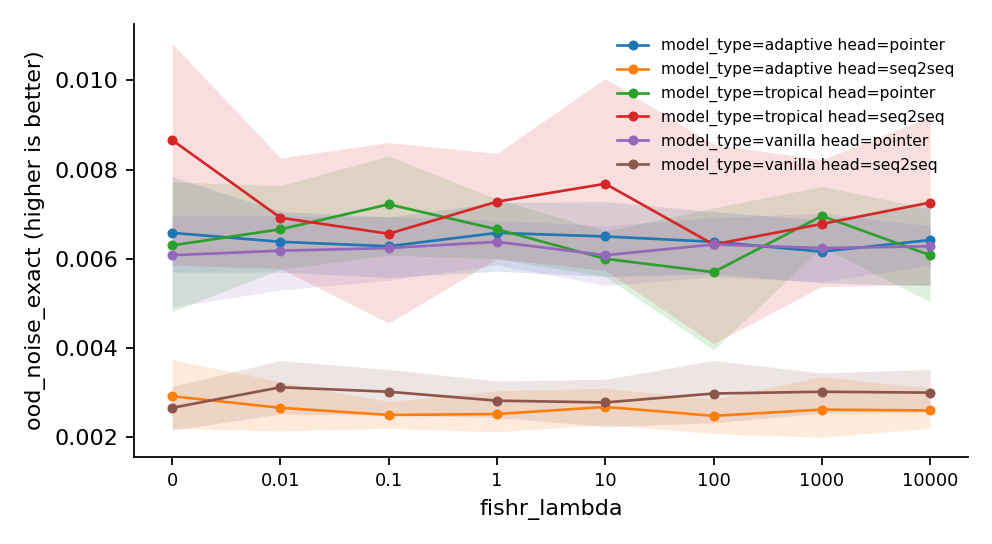
\includegraphics[width=\textwidth]{metric_ood_noise_exact.png}
\caption{\texttt{ood\_noise\_exact} against \texttt{fishr\_lambda}: the mean over seeds with a 95\% bootstrap CI, one line per combination of the other factors.}
\label{fig:ood_noise_exact}
\end{figure}

{\small
\begin{longtable}{lllrlrrr}
\caption{\texttt{ood\_noise\_exact} per cell: mean, 95\% bootstrap CI, SD, seeds, diverged runs.}\label{tab:summary-ood_noise_exact}\\
\toprule
\texttt{model\_type} & \texttt{head} & \texttt{fishr\_lambda} & mean & 95\% CI & SD & $n$ & div.\\
\midrule
\endhead
adaptive & pointer & 0 & 0.00658 & [0.0057, 0.00784] & 0.00147 & 5 & 0\\
adaptive & pointer & 0.01 & 0.00638 & [0.0057, 0.00706] & $9.09\times10^{-4}$ & 5 & 0\\
adaptive & pointer & 0.1 & 0.00628 & [0.00558, 0.00694] & $8.98\times10^{-4}$ & 5 & 0\\
adaptive & pointer & 1 & 0.00658 & [0.00572, 0.00726] & $9.86\times10^{-4}$ & 5 & 0\\
adaptive & pointer & 10 & 0.0065 & [0.0056, 0.00728] & 0.00106 & 5 & 0\\
adaptive & pointer & 100 & 0.00638 & [0.00566, 0.00706] & $9.36\times10^{-4}$ & 5 & 0\\
adaptive & pointer & 1000 & 0.00616 & [0.00546, 0.00686] & $9.24\times10^{-4}$ & 5 & 0\\
adaptive & pointer & 1e+04 & 0.00642 & [0.0054, 0.00724] & 0.00129 & 5 & 0\\
adaptive & seq2seq & 0 & 0.00292 & [0.0022, 0.00374] & $9.88\times10^{-4}$ & 5 & 0\\
adaptive & seq2seq & 0.01 & 0.00266 & [0.00214, 0.00324] & $7.40\times10^{-4}$ & 5 & 0\\
adaptive & seq2seq & 0.1 & 0.0025 & [0.0022, 0.0028] & $3.87\times10^{-4}$ & 5 & 0\\
adaptive & seq2seq & 1 & 0.00252 & [0.00212, 0.00304] & $6.06\times10^{-4}$ & 5 & 0\\
adaptive & seq2seq & 10 & 0.00268 & [0.00228, 0.0031] & $4.97\times10^{-4}$ & 5 & 0\\
adaptive & seq2seq & 100 & 0.00248 & [0.00208, 0.00286] & $5.07\times10^{-4}$ & 5 & 0\\
adaptive & seq2seq & 1000 & 0.00262 & [0.002, 0.00336] & $8.76\times10^{-4}$ & 5 & 0\\
adaptive & seq2seq & 1e+04 & 0.0026 & [0.0022, 0.0031] & $5.70\times10^{-4}$ & 5 & 0\\
tropical & pointer & 0 & 0.0063 & [0.00482, 0.00772] & 0.00202 & 5 & 0\\
tropical & pointer & 0.01 & 0.00666 & [0.00576, 0.00764] & 0.00122 & 5 & 0\\
tropical & pointer & 0.1 & 0.00722 & [0.00608, 0.0083] & 0.00146 & 5 & 0\\
tropical & pointer & 1 & 0.00666 & [0.006, 0.00734] & $8.65\times10^{-4}$ & 5 & 0\\
tropical & pointer & 10 & 0.006 & [0.0056, 0.00662] & $6.89\times10^{-4}$ & 5 & 0\\
tropical & pointer & 100 & 0.0057 & [0.00396, 0.00714] & 0.002 & 5 & 0\\
tropical & pointer & 1000 & 0.00696 & [0.00626, 0.00762] & $8.93\times10^{-4}$ & 5 & 0\\
tropical & pointer & 1e+04 & 0.00608 & [0.00504, 0.00712] & 0.00133 & 5 & 0\\
tropical & seq2seq & 0 & 0.00866 & [0.00586, 0.0108] & 0.00326 & 5 & 0\\
tropical & seq2seq & 0.01 & 0.00692 & [0.00578, 0.00826] & 0.00171 & 5 & 0\\
tropical & seq2seq & 0.1 & 0.00656 & [0.00456, 0.0086] & 0.00267 & 5 & 0\\
tropical & seq2seq & 1 & 0.00728 & [0.006, 0.00836] & 0.00152 & 5 & 0\\
tropical & seq2seq & 10 & 0.00768 & [0.00574, 0.01] & 0.00274 & 5 & 0\\
tropical & seq2seq & 100 & 0.00632 & [0.0041, 0.00856] & 0.00291 & 5 & 0\\
tropical & seq2seq & 1000 & 0.00678 & [0.00538, 0.00822] & 0.0019 & 5 & 0\\
tropical & seq2seq & 1e+04 & 0.00726 & [0.00542, 0.00918] & 0.00236 & 5 & 0\\
vanilla & pointer & 0 & 0.00608 & [0.00492, 0.00698] & 0.00133 & 5 & 0\\
vanilla & pointer & 0.01 & 0.00618 & [0.0053, 0.00696] & 0.00105 & 5 & 0\\
vanilla & pointer & 0.1 & 0.00624 & [0.00552, 0.00694] & $9.69\times10^{-4}$ & 5 & 0\\
vanilla & pointer & 1 & 0.00638 & [0.00586, 0.00686] & $6.57\times10^{-4}$ & 5 & 0\\
vanilla & pointer & 10 & 0.00608 & [0.0054, 0.00674] & $8.87\times10^{-4}$ & 5 & 0\\
vanilla & pointer & 100 & 0.00632 & [0.0056, 0.00692] & $8.35\times10^{-4}$ & 5 & 0\\
vanilla & pointer & 1000 & 0.00624 & [0.00548, 0.00702] & 0.001 & 5 & 0\\
vanilla & pointer & 1e+04 & 0.00628 & [0.00586, 0.00674] & $5.63\times10^{-4}$ & 5 & 0\\
vanilla & seq2seq & 0 & 0.00266 & [0.00216, 0.00314] & $6.43\times10^{-4}$ & 5 & 0\\
vanilla & seq2seq & 0.01 & 0.00312 & [0.00252, 0.00372] & $8.29\times10^{-4}$ & 5 & 0\\
vanilla & seq2seq & 0.1 & 0.00302 & [0.0025, 0.00352] & $6.94\times10^{-4}$ & 5 & 0\\
vanilla & seq2seq & 1 & 0.00282 & [0.00244, 0.00326] & $5.12\times10^{-4}$ & 5 & 0\\
vanilla & seq2seq & 10 & 0.00278 & [0.00224, 0.0033] & $6.61\times10^{-4}$ & 5 & 0\\
vanilla & seq2seq & 100 & 0.00298 & [0.00232, 0.00372] & $9.26\times10^{-4}$ & 5 & 0\\
vanilla & seq2seq & 1000 & 0.00302 & [0.00254, 0.00344] & $5.85\times10^{-4}$ & 5 & 0\\
vanilla & seq2seq & 1e+04 & 0.003 & [0.00256, 0.00352] & $6.28\times10^{-4}$ & 5 & 0\\
\bottomrule
\end{longtable}
}

{\small
\begin{longtable}{lllrrrl}
\caption{\texttt{ood\_noise\_exact}: each level of \texttt{fishr\_lambda} against its control (0), within each combination of the other factors. rank: Wilcoxon signed-rank by seed, Holm.}\label{tab:control-ood_noise_exact}\\
\toprule
\texttt{model\_type} & \texttt{head} & \texttt{fishr\_lambda} & difference & 95\% CI & $p$ & \\
\midrule
\endhead
adaptive & pointer & 0.01 & $-1.000\times10^{-4}$ & [-0.00102, $4.20\times10^{-4}$] & 1.0000 & \\
adaptive & pointer & 0.1 & $-1.000\times10^{-4}$ & [-0.00128, $4.60\times10^{-4}$] & 1.0000 & \\
adaptive & pointer & 1 & $4.000\times10^{-4}$ & [$-8.40\times10^{-4}$, $7.20\times10^{-4}$] & 1.0000 & \\
adaptive & pointer & 10 & $3.000\times10^{-4}$ & [$-8.60\times10^{-4}$, $5.40\times10^{-4}$] & 1.0000 & \\
adaptive & pointer & 100 & $2.000\times10^{-4}$ & [$-9.40\times10^{-4}$, $3.60\times10^{-4}$] & 1.0000 & \\
adaptive & pointer & 1000 & $-1.000\times10^{-4}$ & [-0.00118, $1.80\times10^{-4}$] & 1.0000 & \\
adaptive & pointer & 1e+04 & $3.000\times10^{-4}$ & [$-9.80\times10^{-4}$, $6.60\times10^{-4}$] & 1.0000 & \\
adaptive & seq2seq & 0.01 & $-2.000\times10^{-4}$ & [-0.00116, $6.40\times10^{-4}$] & 1.0000 & \\
adaptive & seq2seq & 0.1 & $-1.000\times10^{-4}$ & [-0.00134, $3.60\times10^{-4}$] & 1.0000 & \\
adaptive & seq2seq & 1 & $-2.000\times10^{-4}$ & [-0.00148, $5.60\times10^{-4}$] & 1.0000 & \\
adaptive & seq2seq & 10 & $-2.000\times10^{-4}$ & [-0.0011, $5.00\times10^{-4}$] & 1.0000 & \\
adaptive & seq2seq & 100 & $1.000\times10^{-4}$ & [-0.00144, $1.80\times10^{-4}$] & 1.0000 & \\
adaptive & seq2seq & 1000 & $1.000\times10^{-4}$ & [-0.00146, $5.00\times10^{-4}$] & 1.0000 & \\
adaptive & seq2seq & 1e+04 & $1.000\times10^{-4}$ & [-0.00116, $1.40\times10^{-4}$] & 1.0000 & \\
tropical & pointer & 0.01 & $5.000\times10^{-4}$ & [$-3.00\times10^{-4}$, 0.001] & 1.0000 & \\
tropical & pointer & 0.1 & $8.000\times10^{-4}$ & [$5.20\times10^{-4}$, 0.00148] & 0.4375 & \\
tropical & pointer & 1 & $5.000\times10^{-4}$ & [$-6.20\times10^{-4}$, 0.0014] & 1.0000 & \\
tropical & pointer & 10 & -0.001 & [-0.00132, $9.80\times10^{-4}$] & 1.0000 & \\
tropical & pointer & 100 & $-5.000\times10^{-4}$ & [-0.0018, $5.20\times10^{-4}$] & 1.0000 & \\
tropical & pointer & 1000 & $3.000\times10^{-4}$ & [$-8.80\times10^{-4}$, 0.00276] & 1.0000 & \\
tropical & pointer & 1e+04 & $4.000\times10^{-4}$ & [-0.00196, $8.20\times10^{-4}$] & 1.0000 & \\
tropical & seq2seq & 0.01 & -0.0032 & [-0.0048, 0.00132] & 1.0000 & \\
tropical & seq2seq & 0.1 & -0.0021 & [-0.00482, $8.42\times10^{-4}$] & 1.0000 & \\
tropical & seq2seq & 1 & -0.0011 & [-0.00362, 0.00114] & 1.0000 & \\
tropical & seq2seq & 10 & $-4.000\times10^{-4}$ & [-0.00328, 0.00132] & 1.0000 & \\
tropical & seq2seq & 100 & -0.0032 & [-0.00452, $-1.20\times10^{-4}$] & 1.0000 & \\
tropical & seq2seq & 1000 & -0.0022 & [-0.00476, $8.00\times10^{-4}$] & 1.0000 & \\
tropical & seq2seq & 1e+04 & -0.0012 & [-0.00258, $-2.60\times10^{-4}$] & 0.8750 & \\
vanilla & pointer & 0.01 & $1.000\times10^{-4}$ & [-0.00106, 0.00142] & 1.0000 & \\
vanilla & pointer & 0.1 & $-2.000\times10^{-4}$ & [$-9.20\times10^{-4}$, 0.00152] & 1.0000 & \\
vanilla & pointer & 1 & 0 & [$-7.60\times10^{-4}$, 0.00154] & 1.0000 & \\
vanilla & pointer & 10 & $-1.000\times10^{-4}$ & [-0.00102, 0.00122] & 1.0000 & \\
vanilla & pointer & 100 & $-1.000\times10^{-4}$ & [$-8.20\times10^{-4}$, 0.00164] & 1.0000 & \\
vanilla & pointer & 1000 & $-3.000\times10^{-4}$ & [$-9.00\times10^{-4}$, 0.00146] & 1.0000 & \\
vanilla & pointer & 1e+04 & 0 & [$-7.60\times10^{-4}$, 0.00124] & 1.0000 & \\
vanilla & seq2seq & 0.01 & $3.000\times10^{-4}$ & [$2.00\times10^{-5}$, $9.60\times10^{-4}$] & 1.0000 & \\
vanilla & seq2seq & 0.1 & $5.000\times10^{-4}$ & [$-2.00\times10^{-4}$, $8.60\times10^{-4}$] & 1.0000 & \\
vanilla & seq2seq & 1 & $1.000\times10^{-4}$ & [$-2.20\times10^{-4}$, $5.20\times10^{-4}$] & 1.0000 & \\
vanilla & seq2seq & 10 & 0 & [$-3.80\times10^{-4}$, $7.00\times10^{-4}$] & 1.0000 & \\
vanilla & seq2seq & 100 & $4.000\times10^{-4}$ & [$-3.20\times10^{-4}$, $8.40\times10^{-4}$] & 1.0000 & \\
vanilla & seq2seq & 1000 & $1.000\times10^{-4}$ & [$-2.20\times10^{-4}$, $1.00\times10^{-3}$] & 1.0000 & \\
vanilla & seq2seq & 1e+04 & $2.000\times10^{-4}$ & [$1.20\times10^{-4}$, $5.80\times10^{-4}$] & 0.8750 & \\
\bottomrule
\end{longtable}
}

{\small
\begin{longtable}{llrrrrr}
\caption{\texttt{ood\_noise\_exact} against log10 \texttt{fishr\_lambda}: rank: Spearman rho, seed-bootstrap CI, with the Jonckheere--Terpstra ordered-trend $\tau$ and $p$.}\label{tab:trend-ood_noise_exact}\\
\toprule
\texttt{model\_type} & \texttt{head} & estimate & 95\% CI & $p$ & JT $\tau$ & JT $p$\\
\midrule
\endhead
adaptive & pointer & -0.05529 & [-0.375, 0.185] & 0.7524 & -0.0514 & 0.7119\\
adaptive & seq2seq & -0.03552 & [-0.544, 0.523] & 0.8395 & -0.0343 & 0.8072\\
tropical & pointer & -0.1536 & [-0.516, 0.0426] & 0.3783 & -0.122 & 0.3573\\
tropical & seq2seq & 0.02618 & [-0.315, 0.318] & 0.8813 & 0.0133 & 0.9278\\
vanilla & pointer & 0.002126 & [-0.329, 0.327] & 0.9903 & -0.0019 & 0.9954\\
vanilla & seq2seq & -0.01985 & [-0.159, 0.129] & 0.9099 & -0.0171 & 0.9020\\
\bottomrule
\end{longtable}
}

{\small
\begin{longtable}{lrrrl}
\caption{\texttt{ood\_noise\_exact}: paired contrasts by seed, Holm-corrected across the cells. rank: Wilcoxon signed-rank by seed, Holm.}\label{tab:paired-ood_noise_exact}\\
\toprule
contrast (within) & difference & 95\% CI & $p$ & \\
\midrule
\endhead
\stackcell{model\_type: tropical - vanilla\\\footnotesize head=pointer fishr\_lambda=0 } & $2.200\times10^{-4}$ & [-0.00185, 0.00229] & 1.0000 & \\
\stackcell{model\_type: tropical - vanilla\\\footnotesize head=pointer fishr\_lambda=0.01 } & $4.800\times10^{-4}$ & [-0.00112, 0.00208] & 1.0000 & \\
\stackcell{model\_type: tropical - vanilla\\\footnotesize head=pointer fishr\_lambda=0.1 } & $9.800\times10^{-4}$ & [$-8.22\times10^{-4}$, 0.00278] & 1.0000 & \\
\stackcell{model\_type: tropical - vanilla\\\footnotesize head=pointer fishr\_lambda=1 } & $2.800\times10^{-4}$ & [$-8.66\times10^{-4}$, 0.00143] & 1.0000 & \\
\stackcell{model\_type: tropical - vanilla\\\footnotesize head=pointer fishr\_lambda=10 } & $-8.000\times10^{-5}$ & [-0.00155, 0.00139] & 1.0000 & \\
\stackcell{model\_type: tropical - vanilla\\\footnotesize head=pointer fishr\_lambda=100 } & $-6.200\times10^{-4}$ & [-0.00342, 0.00218] & 1.0000 & \\
\stackcell{model\_type: tropical - vanilla\\\footnotesize head=pointer fishr\_lambda=1000 } & $7.200\times10^{-4}$ & [-0.00111, 0.00255] & 1.0000 & \\
\stackcell{model\_type: tropical - vanilla\\\footnotesize head=pointer fishr\_lambda=1e+04 } & $-2.000\times10^{-4}$ & [-0.00123, $8.28\times10^{-4}$] & 1.0000 & \\
\stackcell{model\_type: tropical - vanilla\\\footnotesize head=seq2seq fishr\_lambda=0 } & 0.006 & [0.00221, 0.00979] & 1.0000 & \\
\stackcell{model\_type: tropical - vanilla\\\footnotesize head=seq2seq fishr\_lambda=0.01 } & 0.0038 & [0.00125, 0.00635] & 1.0000 & \\
\stackcell{model\_type: tropical - vanilla\\\footnotesize head=seq2seq fishr\_lambda=0.1 } & 0.00354 & [$1.32\times10^{-4}$, 0.00695] & 1.0000 & \\
\stackcell{model\_type: tropical - vanilla\\\footnotesize head=seq2seq fishr\_lambda=1 } & 0.00446 & [0.00211, 0.00681] & 1.0000 & \\
\stackcell{model\_type: tropical - vanilla\\\footnotesize head=seq2seq fishr\_lambda=10 } & 0.0049 & [$8.80\times10^{-4}$, 0.00892] & 1.0000 & \\
\stackcell{model\_type: tropical - vanilla\\\footnotesize head=seq2seq fishr\_lambda=100 } & 0.00334 & [$-8.84\times10^{-4}$, 0.00756] & 1.0000 & \\
\stackcell{model\_type: tropical - vanilla\\\footnotesize head=seq2seq fishr\_lambda=1000 } & 0.00376 & [0.0013, 0.00622] & 1.0000 & \\
\stackcell{model\_type: tropical - vanilla\\\footnotesize head=seq2seq fishr\_lambda=1e+04 } & 0.00426 & [0.00156, 0.00696] & 1.0000 & \\
\stackcell{model\_type: adaptive - vanilla\\\footnotesize head=pointer fishr\_lambda=0 } & $5.000\times10^{-4}$ & [-0.00102, 0.00202] & 1.0000 & \\
\stackcell{model\_type: adaptive - vanilla\\\footnotesize head=pointer fishr\_lambda=0.01 } & $2.000\times10^{-4}$ & [$-9.94\times10^{-4}$, 0.00139] & 1.0000 & \\
\stackcell{model\_type: adaptive - vanilla\\\footnotesize head=pointer fishr\_lambda=0.1 } & $4.000\times10^{-5}$ & [-0.00109, 0.00117] & 1.0000 & \\
\stackcell{model\_type: adaptive - vanilla\\\footnotesize head=pointer fishr\_lambda=1 } & $2.000\times10^{-4}$ & [-0.00115, 0.00155] & 1.0000 & \\
\stackcell{model\_type: adaptive - vanilla\\\footnotesize head=pointer fishr\_lambda=10 } & $4.200\times10^{-4}$ & [$-9.36\times10^{-4}$, 0.00178] & 1.0000 & \\
\stackcell{model\_type: adaptive - vanilla\\\footnotesize head=pointer fishr\_lambda=100 } & $6.000\times10^{-5}$ & [-0.00132, 0.00144] & 1.0000 & \\
\stackcell{model\_type: adaptive - vanilla\\\footnotesize head=pointer fishr\_lambda=1000 } & $-8.000\times10^{-5}$ & [-0.00153, 0.00137] & 1.0000 & \\
\stackcell{model\_type: adaptive - vanilla\\\footnotesize head=pointer fishr\_lambda=1e+04 } & $1.400\times10^{-4}$ & [-0.0013, 0.00158] & 1.0000 & \\
\stackcell{model\_type: adaptive - vanilla\\\footnotesize head=seq2seq fishr\_lambda=0 } & $2.600\times10^{-4}$ & [-0.00137, 0.00189] & 1.0000 & \\
\stackcell{model\_type: adaptive - vanilla\\\footnotesize head=seq2seq fishr\_lambda=0.01 } & $-4.600\times10^{-4}$ & [-0.00203, 0.00111] & 1.0000 & \\
\stackcell{model\_type: adaptive - vanilla\\\footnotesize head=seq2seq fishr\_lambda=0.1 } & $-5.200\times10^{-4}$ & [-0.00144, $3.98\times10^{-4}$] & 1.0000 & \\
\stackcell{model\_type: adaptive - vanilla\\\footnotesize head=seq2seq fishr\_lambda=1 } & $-3.000\times10^{-4}$ & [-0.00134, $7.39\times10^{-4}$] & 1.0000 & \\
\stackcell{model\_type: adaptive - vanilla\\\footnotesize head=seq2seq fishr\_lambda=10 } & $-1.000\times10^{-4}$ & [-0.0011, $9.01\times10^{-4}$] & 1.0000 & \\
\stackcell{model\_type: adaptive - vanilla\\\footnotesize head=seq2seq fishr\_lambda=100 } & $-5.000\times10^{-4}$ & [-0.00179, $7.93\times10^{-4}$] & 1.0000 & \\
\stackcell{model\_type: adaptive - vanilla\\\footnotesize head=seq2seq fishr\_lambda=1000 } & $-4.000\times10^{-4}$ & [-0.00116, $3.60\times10^{-4}$] & 1.0000 & \\
\stackcell{model\_type: adaptive - vanilla\\\footnotesize head=seq2seq fishr\_lambda=1e+04 } & $-4.000\times10^{-4}$ & [-0.00107, $2.74\times10^{-4}$] & 1.0000 & \\
\stackcell{head: pointer - seq2seq\\\footnotesize model\_type=adaptive fishr\_lambda=0 } & 0.00366 & [0.00153, 0.00579] & 1.0000 & \\
\stackcell{head: pointer - seq2seq\\\footnotesize model\_type=adaptive fishr\_lambda=0.01 } & 0.00372 & [0.00241, 0.00503] & 1.0000 & \\
\stackcell{head: pointer - seq2seq\\\footnotesize model\_type=adaptive fishr\_lambda=0.1 } & 0.00378 & [0.00288, 0.00468] & 1.0000 & \\
\stackcell{head: pointer - seq2seq\\\footnotesize model\_type=adaptive fishr\_lambda=1 } & 0.00406 & [0.00279, 0.00533] & 1.0000 & \\
\stackcell{head: pointer - seq2seq\\\footnotesize model\_type=adaptive fishr\_lambda=10 } & 0.00382 & [0.00257, 0.00507] & 1.0000 & \\
\stackcell{head: pointer - seq2seq\\\footnotesize model\_type=adaptive fishr\_lambda=100 } & 0.0039 & [0.0032, 0.0046] & 1.0000 & \\
\stackcell{head: pointer - seq2seq\\\footnotesize model\_type=adaptive fishr\_lambda=1000 } & 0.00354 & [0.00286, 0.00422] & 1.0000 & \\
\stackcell{head: pointer - seq2seq\\\footnotesize model\_type=adaptive fishr\_lambda=1e+04 } & 0.00382 & [0.00248, 0.00516] & 1.0000 & \\
\stackcell{head: pointer - seq2seq\\\footnotesize model\_type=tropical fishr\_lambda=0 } & -0.00236 & [-0.00693, 0.00221] & 1.0000 & \\
\stackcell{head: pointer - seq2seq\\\footnotesize model\_type=tropical fishr\_lambda=0.01 } & $-2.600\times10^{-4}$ & [-0.0019, 0.00138] & 1.0000 & \\
\stackcell{head: pointer - seq2seq\\\footnotesize model\_type=tropical fishr\_lambda=0.1 } & $6.600\times10^{-4}$ & [-0.00191, 0.00323] & 1.0000 & \\
\stackcell{head: pointer - seq2seq\\\footnotesize model\_type=tropical fishr\_lambda=1 } & $-6.200\times10^{-4}$ & [-0.00303, 0.00179] & 1.0000 & \\
\stackcell{head: pointer - seq2seq\\\footnotesize model\_type=tropical fishr\_lambda=10 } & -0.00168 & [-0.00488, 0.00152] & 1.0000 & \\
\stackcell{head: pointer - seq2seq\\\footnotesize model\_type=tropical fishr\_lambda=100 } & $-6.200\times10^{-4}$ & [-0.00274, 0.0015] & 1.0000 & \\
\stackcell{head: pointer - seq2seq\\\footnotesize model\_type=tropical fishr\_lambda=1000 } & $1.800\times10^{-4}$ & [-0.00204, 0.0024] & 1.0000 & \\
\stackcell{head: pointer - seq2seq\\\footnotesize model\_type=tropical fishr\_lambda=1e+04 } & -0.00118 & [-0.00353, 0.00117] & 1.0000 & \\
\stackcell{head: pointer - seq2seq\\\footnotesize model\_type=vanilla fishr\_lambda=0 } & 0.00342 & [0.00187, 0.00497] & 1.0000 & \\
\stackcell{head: pointer - seq2seq\\\footnotesize model\_type=vanilla fishr\_lambda=0.01 } & 0.00306 & [0.00132, 0.0048] & 1.0000 & \\
\stackcell{head: pointer - seq2seq\\\footnotesize model\_type=vanilla fishr\_lambda=0.1 } & 0.00322 & [0.00212, 0.00432] & 1.0000 & \\
\stackcell{head: pointer - seq2seq\\\footnotesize model\_type=vanilla fishr\_lambda=1 } & 0.00356 & [0.00283, 0.00429] & 1.0000 & \\
\stackcell{head: pointer - seq2seq\\\footnotesize model\_type=vanilla fishr\_lambda=10 } & 0.0033 & [0.0018, 0.0048] & 1.0000 & \\
\stackcell{head: pointer - seq2seq\\\footnotesize model\_type=vanilla fishr\_lambda=100 } & 0.00334 & [0.00172, 0.00496] & 1.0000 & \\
\stackcell{head: pointer - seq2seq\\\footnotesize model\_type=vanilla fishr\_lambda=1000 } & 0.00322 & [0.00211, 0.00433] & 1.0000 & \\
\stackcell{head: pointer - seq2seq\\\footnotesize model\_type=vanilla fishr\_lambda=1e+04 } & 0.00328 & [0.00236, 0.0042] & 1.0000 & \\
\bottomrule
\end{longtable}
}

\subsection{\texttt{id\_f1}}
\begin{figure}[tbp]
\centering
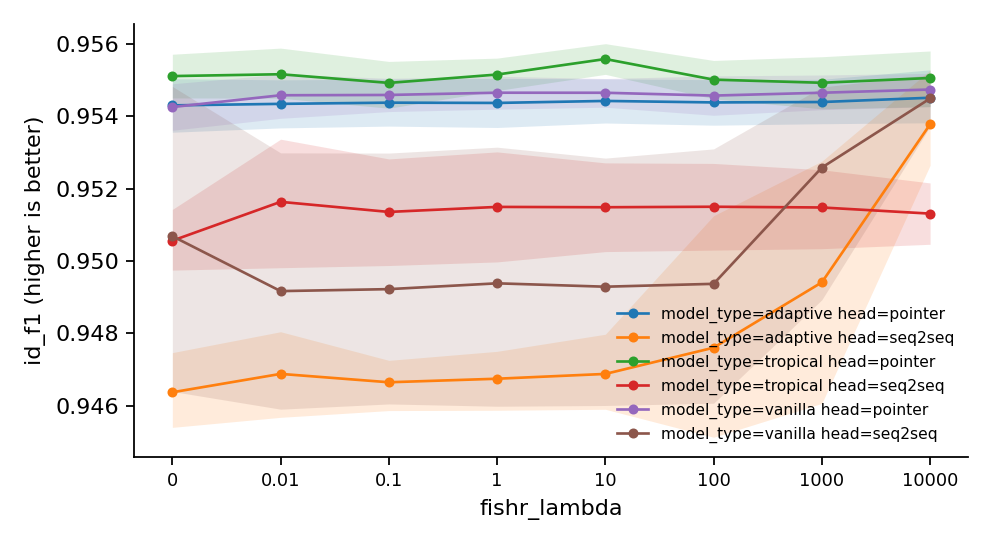
\includegraphics[width=\textwidth]{metric_id_f1.png}
\caption{\texttt{id\_f1} against \texttt{fishr\_lambda}: the mean over seeds with a 95\% bootstrap CI, one line per combination of the other factors.}
\label{fig:id_f1}
\end{figure}

{\small
\begin{longtable}{lllrlrrr}
\caption{\texttt{id\_f1} per cell: mean, 95\% bootstrap CI, SD, seeds, diverged runs.}\label{tab:summary-id_f1}\\
\toprule
\texttt{model\_type} & \texttt{head} & \texttt{fishr\_lambda} & mean & 95\% CI & SD & $n$ & div.\\
\midrule
\endhead
adaptive & pointer & 0 & 0.9543 & [0.954, 0.955] & 0.00105 & 5 & 0\\
adaptive & pointer & 0.01 & 0.9543 & [0.954, 0.955] & $8.67\times10^{-4}$ & 5 & 0\\
adaptive & pointer & 0.1 & 0.9544 & [0.954, 0.955] & $8.61\times10^{-4}$ & 5 & 0\\
adaptive & pointer & 1 & 0.9544 & [0.954, 0.955] & $8.85\times10^{-4}$ & 5 & 0\\
adaptive & pointer & 10 & 0.9544 & [0.954, 0.955] & $7.79\times10^{-4}$ & 5 & 0\\
adaptive & pointer & 100 & 0.9544 & [0.954, 0.955] & $8.35\times10^{-4}$ & 5 & 0\\
adaptive & pointer & 1000 & 0.9544 & [0.954, 0.955] & $8.06\times10^{-4}$ & 5 & 0\\
adaptive & pointer & 1e+04 & 0.9545 & [0.954, 0.955] & $9.38\times10^{-4}$ & 5 & 0\\
adaptive & seq2seq & 0 & 0.9464 & [0.945, 0.947] & 0.00133 & 5 & 0\\
adaptive & seq2seq & 0.01 & 0.9469 & [0.946, 0.948] & 0.0015 & 5 & 0\\
adaptive & seq2seq & 0.1 & 0.9466 & [0.946, 0.947] & $8.86\times10^{-4}$ & 5 & 0\\
adaptive & seq2seq & 1 & 0.9467 & [0.946, 0.948] & 0.00109 & 5 & 0\\
adaptive & seq2seq & 10 & 0.9469 & [0.946, 0.948] & 0.0014 & 5 & 0\\
adaptive & seq2seq & 100 & 0.9476 & [0.945, 0.951] & 0.00411 & 5 & 0\\
adaptive & seq2seq & 1000 & 0.9494 & [0.946, 0.953] & 0.00435 & 5 & 0\\
adaptive & seq2seq & 1e+04 & 0.9538 & [0.953, 0.955] & 0.00168 & 5 & 0\\
tropical & pointer & 0 & 0.9551 & [0.955, 0.956] & $7.67\times10^{-4}$ & 5 & 0\\
tropical & pointer & 0.01 & 0.9552 & [0.954, 0.956] & $8.82\times10^{-4}$ & 5 & 0\\
tropical & pointer & 0.1 & 0.9549 & [0.954, 0.956] & $8.21\times10^{-4}$ & 5 & 0\\
tropical & pointer & 1 & 0.9552 & [0.955, 0.956] & $5.96\times10^{-4}$ & 5 & 0\\
tropical & pointer & 10 & 0.9556 & [0.955, 0.956] & $5.70\times10^{-4}$ & 5 & 0\\
tropical & pointer & 100 & 0.955 & [0.954, 0.956] & $7.12\times10^{-4}$ & 5 & 0\\
tropical & pointer & 1000 & 0.9549 & [0.954, 0.956] & $9.27\times10^{-4}$ & 5 & 0\\
tropical & pointer & 1e+04 & 0.9551 & [0.954, 0.956] & 0.00102 & 5 & 0\\
tropical & seq2seq & 0 & 0.9506 & [0.95, 0.951] & 0.00101 & 5 & 0\\
tropical & seq2seq & 0.01 & 0.9516 & [0.95, 0.953] & 0.00234 & 5 & 0\\
tropical & seq2seq & 0.1 & 0.9514 & [0.95, 0.953] & 0.00183 & 5 & 0\\
tropical & seq2seq & 1 & 0.9515 & [0.95, 0.953] & 0.00199 & 5 & 0\\
tropical & seq2seq & 10 & 0.9515 & [0.95, 0.953] & 0.00161 & 5 & 0\\
tropical & seq2seq & 100 & 0.9515 & [0.95, 0.953] & 0.00165 & 5 & 0\\
tropical & seq2seq & 1000 & 0.9515 & [0.95, 0.953] & 0.00144 & 5 & 0\\
tropical & seq2seq & 1e+04 & 0.9513 & [0.95, 0.952] & 0.00113 & 5 & 0\\
vanilla & pointer & 0 & 0.9543 & [0.954, 0.955] & $8.38\times10^{-4}$ & 5 & 0\\
vanilla & pointer & 0.01 & 0.9546 & [0.954, 0.955] & $7.77\times10^{-4}$ & 5 & 0\\
vanilla & pointer & 0.1 & 0.9546 & [0.954, 0.955] & $5.87\times10^{-4}$ & 5 & 0\\
vanilla & pointer & 1 & 0.9546 & [0.954, 0.955] & $5.82\times10^{-4}$ & 5 & 0\\
vanilla & pointer & 10 & 0.9546 & [0.954, 0.955] & $5.16\times10^{-4}$ & 5 & 0\\
vanilla & pointer & 100 & 0.9546 & [0.954, 0.955] & $6.99\times10^{-4}$ & 5 & 0\\
vanilla & pointer & 1000 & 0.9546 & [0.954, 0.955] & $6.32\times10^{-4}$ & 5 & 0\\
vanilla & pointer & 1e+04 & 0.9547 & [0.954, 0.955] & $6.05\times10^{-4}$ & 5 & 0\\
vanilla & seq2seq & 0 & 0.9507 & [0.946, 0.955] & 0.00551 & 5 & 0\\
vanilla & seq2seq & 0.01 & 0.9492 & [0.946, 0.953] & 0.00453 & 5 & 0\\
vanilla & seq2seq & 0.1 & 0.9492 & [0.946, 0.953] & 0.00444 & 5 & 0\\
vanilla & seq2seq & 1 & 0.9494 & [0.946, 0.953] & 0.00462 & 5 & 0\\
vanilla & seq2seq & 10 & 0.9493 & [0.946, 0.953] & 0.00441 & 5 & 0\\
vanilla & seq2seq & 100 & 0.9494 & [0.946, 0.953] & 0.00451 & 5 & 0\\
vanilla & seq2seq & 1000 & 0.9526 & [0.949, 0.955] & 0.00403 & 5 & 0\\
vanilla & seq2seq & 1e+04 & 0.9545 & [0.954, 0.955] & $9.10\times10^{-4}$ & 5 & 0\\
\bottomrule
\end{longtable}
}

{\small
\begin{longtable}{lllrrrl}
\caption{\texttt{id\_f1}: each level of \texttt{fishr\_lambda} against its control (0), within each combination of the other factors. parametric: Dunnett vs control.}\label{tab:control-id_f1}\\
\toprule
\texttt{model\_type} & \texttt{head} & \texttt{fishr\_lambda} & difference & 95\% CI & $p$ & \\
\midrule
\endhead
adaptive & pointer & 0.01 & $4.184\times10^{-5}$ & [-0.0015, 0.00158] & 1.0000 & \\
adaptive & pointer & 0.1 & $7.518\times10^{-5}$ & [-0.00146, 0.00161] & 1.0000 & \\
adaptive & pointer & 1 & $6.751\times10^{-5}$ & [-0.00147, 0.00161] & 1.0000 & \\
adaptive & pointer & 10 & $1.227\times10^{-4}$ & [-0.00142, 0.00166] & 1.0000 & \\
adaptive & pointer & 100 & $8.134\times10^{-5}$ & [-0.00146, 0.00162] & 1.0000 & \\
adaptive & pointer & 1000 & $9.238\times10^{-5}$ & [-0.00145, 0.00163] & 1.0000 & \\
adaptive & pointer & 1e+04 & $2.109\times10^{-4}$ & [-0.00133, 0.00175] & 0.9992 & \\
adaptive & seq2seq & 0.01 & $5.085\times10^{-4}$ & [-0.00371, 0.00473] & 0.9996 & \\
adaptive & seq2seq & 0.1 & $2.769\times10^{-4}$ & [-0.00394, 0.0045] & 1.0000 & \\
adaptive & seq2seq & 1 & $3.747\times10^{-4}$ & [-0.00384, 0.00459] & 1.0000 & \\
adaptive & seq2seq & 10 & $5.074\times10^{-4}$ & [-0.00371, 0.00473] & 0.9996 & \\
adaptive & seq2seq & 100 & 0.001233 & [-0.00299, 0.00545] & 0.9409 & \\
adaptive & seq2seq & 1000 & 0.003039 & [-0.00118, 0.00726] & 0.2417 & \\
adaptive & seq2seq & 1e+04 & 0.007408 & [0.00319, 0.0116] & 0.0002 & *\\
tropical & pointer & 0.01 & $5.087\times10^{-5}$ & [-0.00135, 0.00145] & 1.0000 & \\
tropical & pointer & 0.1 & $-1.889\times10^{-4}$ & [-0.00159, 0.00121] & 0.9992 & \\
tropical & pointer & 1 & $4.231\times10^{-5}$ & [-0.00136, 0.00144] & 1.0000 & \\
tropical & pointer & 10 & $4.716\times10^{-4}$ & [$-9.27\times10^{-4}$, 0.00187] & 0.8901 & \\
tropical & pointer & 100 & $-9.867\times10^{-5}$ & [-0.0015, 0.0013] & 1.0000 & \\
tropical & pointer & 1000 & $-1.850\times10^{-4}$ & [-0.00158, 0.00121] & 0.9993 & \\
tropical & pointer & 1e+04 & $-5.287\times10^{-5}$ & [-0.00145, 0.00135] & 1.0000 & \\
tropical & seq2seq & 0.01 & 0.001073 & [-0.00185, 0.004] & 0.8473 & \\
tropical & seq2seq & 0.1 & $7.945\times10^{-4}$ & [-0.00213, 0.00372] & 0.9583 & \\
tropical & seq2seq & 1 & $9.333\times10^{-4}$ & [-0.00199, 0.00386] & 0.9129 & \\
tropical & seq2seq & 10 & $9.241\times10^{-4}$ & [-0.002, 0.00385] & 0.9165 & \\
tropical & seq2seq & 100 & $9.379\times10^{-4}$ & [-0.00199, 0.00387] & 0.9110 & \\
tropical & seq2seq & 1000 & $9.176\times10^{-4}$ & [-0.00201, 0.00384] & 0.9190 & \\
tropical & seq2seq & 1e+04 & $7.480\times10^{-4}$ & [-0.00218, 0.00368] & 0.9691 & \\
vanilla & pointer & 0.01 & $3.256\times10^{-4}$ & [$-8.32\times10^{-4}$, 0.00148] & 0.9504 & \\
vanilla & pointer & 0.1 & $3.339\times10^{-4}$ & [$-8.23\times10^{-4}$, 0.00149] & 0.9443 & \\
vanilla & pointer & 1 & $3.962\times10^{-4}$ & [$-7.61\times10^{-4}$, 0.00155] & 0.8830 & \\
vanilla & pointer & 10 & $3.947\times10^{-4}$ & [$-7.63\times10^{-4}$, 0.00155] & 0.8847 & \\
vanilla & pointer & 100 & $3.166\times10^{-4}$ & [$-8.41\times10^{-4}$, 0.00147] & 0.9567 & \\
vanilla & pointer & 1000 & $3.953\times10^{-4}$ & [$-7.62\times10^{-4}$, 0.00155] & 0.8840 & \\
vanilla & pointer & 1e+04 & $4.840\times10^{-4}$ & [$-6.73\times10^{-4}$, 0.00164] & 0.7593 & \\
vanilla & seq2seq & 0.01 & -0.001518 & [-0.00905, 0.00601] & 0.9914 & \\
vanilla & seq2seq & 0.1 & -0.001464 & [-0.009, 0.00607] & 0.9930 & \\
vanilla & seq2seq & 1 & -0.001303 & [-0.00883, 0.00623] & 0.9965 & \\
vanilla & seq2seq & 10 & -0.001396 & [-0.00893, 0.00614] & 0.9947 & \\
vanilla & seq2seq & 100 & -0.001317 & [-0.00885, 0.00621] & 0.9962 & \\
vanilla & seq2seq & 1000 & 0.001896 & [-0.00564, 0.00943] & 0.9713 & \\
vanilla & seq2seq & 1e+04 & 0.003806 & [-0.00373, 0.0113] & 0.5909 & \\
\bottomrule
\end{longtable}
}

{\small
\begin{longtable}{llrrrrr}
\caption{\texttt{id\_f1} against log10 \texttt{fishr\_lambda}: parametric: OLS slope t-test, seed-bootstrap CI, with the Jonckheere--Terpstra ordered-trend $\tau$ and $p$.}\label{tab:trend-id_f1}\\
\toprule
\texttt{model\_type} & \texttt{head} & estimate & 95\% CI & $p$ & JT $\tau$ & JT $p$\\
\midrule
\endhead
adaptive & pointer & $1.983\times10^{-5}$ & [$-1.87\times10^{-5}$, $5.65\times10^{-5}$] & 0.7677 & 0.0514 & 0.7015\\
adaptive & seq2seq & $9.671\times10^{-4}$ & [$7.60\times10^{-4}$, 0.00131] & 0.0002 & 0.284 & 0.0358\\
tropical & pointer & $-1.588\times10^{-5}$ & [$-8.35\times10^{-5}$, $2.28\times10^{-5}$] & 0.8093 & -0.0514 & 0.7101\\
tropical & seq2seq & $-2.590\times10^{-5}$ & [$-1.85\times10^{-4}$, $1.38\times10^{-4}$] & 0.8507 & -0.0514 & 0.7249\\
vanilla & pointer & $1.850\times10^{-5}$ & [$5.44\times10^{-7}$, $3.89\times10^{-5}$] & 0.7106 & 0.0438 & 0.7560\\
vanilla & seq2seq & $8.099\times10^{-4}$ & [$2.67\times10^{-4}$, 0.00135] & 0.0215 & 0.28 & 0.0352\\
\bottomrule
\end{longtable}
}

{\small
\begin{longtable}{lrrrl}
\caption{\texttt{id\_f1}: paired contrasts by seed, Holm-corrected across the cells. parametric: paired t-test by seed, Holm.}\label{tab:paired-id_f1}\\
\toprule
contrast (within) & difference & 95\% CI & $p$ & \\
\midrule
\endhead
\stackcell{model\_type: tropical - vanilla\\\footnotesize head=pointer fishr\_lambda=0 } & $8.558\times10^{-4}$ & [$1.63\times10^{-4}$, 0.00155] & 0.3458 & \\
\stackcell{model\_type: tropical - vanilla\\\footnotesize head=pointer fishr\_lambda=0.01 } & $5.810\times10^{-4}$ & [$1.68\times10^{-4}$, $9.94\times10^{-4}$] & 0.2451 & \\
\stackcell{model\_type: tropical - vanilla\\\footnotesize head=pointer fishr\_lambda=0.1 } & $3.331\times10^{-4}$ & [$-3.50\times10^{-5}$, $7.01\times10^{-4}$] & 0.6588 & \\
\stackcell{model\_type: tropical - vanilla\\\footnotesize head=pointer fishr\_lambda=1 } & $5.019\times10^{-4}$ & [$8.16\times10^{-5}$, $9.22\times10^{-4}$] & 0.3540 & \\
\stackcell{model\_type: tropical - vanilla\\\footnotesize head=pointer fishr\_lambda=10 } & $9.327\times10^{-4}$ & [$6.51\times10^{-4}$, 0.00121] & 0.0124 & *\\
\stackcell{model\_type: tropical - vanilla\\\footnotesize head=pointer fishr\_lambda=100 } & $4.406\times10^{-4}$ & [$4.59\times10^{-5}$, $8.35\times10^{-4}$] & 0.3986 & \\
\stackcell{model\_type: tropical - vanilla\\\footnotesize head=pointer fishr\_lambda=1000 } & $2.754\times10^{-4}$ & [$-2.81\times10^{-4}$, $8.32\times10^{-4}$] & 1.0000 & \\
\stackcell{model\_type: tropical - vanilla\\\footnotesize head=pointer fishr\_lambda=1e+04 } & $3.190\times10^{-4}$ & [$-3.18\times10^{-4}$, $9.56\times10^{-4}$] & 1.0000 & \\
\stackcell{model\_type: tropical - vanilla\\\footnotesize head=seq2seq fishr\_lambda=0 } & $-1.241\times10^{-4}$ & [-0.0062, 0.00595] & 1.0000 & \\
\stackcell{model\_type: tropical - vanilla\\\footnotesize head=seq2seq fishr\_lambda=0.01 } & 0.002467 & [-0.00449, 0.00942] & 1.0000 & \\
\stackcell{model\_type: tropical - vanilla\\\footnotesize head=seq2seq fishr\_lambda=0.1 } & 0.002134 & [-0.00404, 0.00831] & 1.0000 & \\
\stackcell{model\_type: tropical - vanilla\\\footnotesize head=seq2seq fishr\_lambda=1 } & 0.002112 & [-0.00454, 0.00876] & 1.0000 & \\
\stackcell{model\_type: tropical - vanilla\\\footnotesize head=seq2seq fishr\_lambda=10 } & 0.002196 & [-0.0039, 0.0083] & 1.0000 & \\
\stackcell{model\_type: tropical - vanilla\\\footnotesize head=seq2seq fishr\_lambda=100 } & 0.002131 & [-0.00382, 0.00808] & 1.0000 & \\
\stackcell{model\_type: tropical - vanilla\\\footnotesize head=seq2seq fishr\_lambda=1000 } & -0.001103 & [-0.00727, 0.00507] & 1.0000 & \\
\stackcell{model\_type: tropical - vanilla\\\footnotesize head=seq2seq fishr\_lambda=1e+04 } & -0.003182 & [-0.00433, -0.00203] & 0.0233 & *\\
\stackcell{model\_type: adaptive - vanilla\\\footnotesize head=pointer fishr\_lambda=0 } & $4.603\times10^{-5}$ & [$-8.79\times10^{-4}$, $9.71\times10^{-4}$] & 1.0000 & \\
\stackcell{model\_type: adaptive - vanilla\\\footnotesize head=pointer fishr\_lambda=0.01 } & $-2.378\times10^{-4}$ & [$-5.31\times10^{-4}$, $5.54\times10^{-5}$] & 1.0000 & \\
\stackcell{model\_type: adaptive - vanilla\\\footnotesize head=pointer fishr\_lambda=0.1 } & $-2.127\times10^{-4}$ & [$-6.03\times10^{-4}$, $1.77\times10^{-4}$] & 1.0000 & \\
\stackcell{model\_type: adaptive - vanilla\\\footnotesize head=pointer fishr\_lambda=1 } & $-2.826\times10^{-4}$ & [$-6.72\times10^{-4}$, $1.07\times10^{-4}$] & 1.0000 & \\
\stackcell{model\_type: adaptive - vanilla\\\footnotesize head=pointer fishr\_lambda=10 } & $-2.260\times10^{-4}$ & [$-5.64\times10^{-4}$, $1.12\times10^{-4}$] & 1.0000 & \\
\stackcell{model\_type: adaptive - vanilla\\\footnotesize head=pointer fishr\_lambda=100 } & $-1.892\times10^{-4}$ & [$-4.82\times10^{-4}$, $1.04\times10^{-4}$] & 1.0000 & \\
\stackcell{model\_type: adaptive - vanilla\\\footnotesize head=pointer fishr\_lambda=1000 } & $-2.569\times10^{-4}$ & [$-4.91\times10^{-4}$, $-2.27\times10^{-5}$] & 0.6114 & \\
\stackcell{model\_type: adaptive - vanilla\\\footnotesize head=pointer fishr\_lambda=1e+04 } & $-2.271\times10^{-4}$ & [$-9.04\times10^{-4}$, $4.50\times10^{-4}$] & 1.0000 & \\
\stackcell{model\_type: adaptive - vanilla\\\footnotesize head=seq2seq fishr\_lambda=0 } & -0.004315 & [-0.0102, 0.00153] & 1.0000 & \\
\stackcell{model\_type: adaptive - vanilla\\\footnotesize head=seq2seq fishr\_lambda=0.01 } & -0.002288 & [-0.00778, 0.00321] & 1.0000 & \\
\stackcell{model\_type: adaptive - vanilla\\\footnotesize head=seq2seq fishr\_lambda=0.1 } & -0.002574 & [-0.0084, 0.00325] & 1.0000 & \\
\stackcell{model\_type: adaptive - vanilla\\\footnotesize head=seq2seq fishr\_lambda=1 } & -0.002637 & [-0.00857, 0.00329] & 1.0000 & \\
\stackcell{model\_type: adaptive - vanilla\\\footnotesize head=seq2seq fishr\_lambda=10 } & -0.002411 & [-0.00766, 0.00283] & 1.0000 & \\
\stackcell{model\_type: adaptive - vanilla\\\footnotesize head=seq2seq fishr\_lambda=100 } & -0.001765 & [-0.00609, 0.00256] & 1.0000 & \\
\stackcell{model\_type: adaptive - vanilla\\\footnotesize head=seq2seq fishr\_lambda=1000 } & -0.003172 & [-0.0114, 0.00504] & 1.0000 & \\
\stackcell{model\_type: adaptive - vanilla\\\footnotesize head=seq2seq fishr\_lambda=1e+04 } & $-7.130\times10^{-4}$ & [-0.00183, $4.02\times10^{-4}$] & 1.0000 & \\
\stackcell{head: pointer - seq2seq\\\footnotesize model\_type=adaptive fishr\_lambda=0 } & 0.00793 & [0.00621, 0.00965] & 0.0038 & *\\
\stackcell{head: pointer - seq2seq\\\footnotesize model\_type=adaptive fishr\_lambda=0.01 } & 0.007464 & [0.00614, 0.00879] & 0.0019 & *\\
\stackcell{head: pointer - seq2seq\\\footnotesize model\_type=adaptive fishr\_lambda=0.1 } & 0.007729 & [0.0066, 0.00886] & 0.0010 & *\\
\stackcell{head: pointer - seq2seq\\\footnotesize model\_type=adaptive fishr\_lambda=1 } & 0.007623 & [0.00672, 0.00852] & 0.0005 & *\\
\stackcell{head: pointer - seq2seq\\\footnotesize model\_type=adaptive fishr\_lambda=10 } & 0.007546 & [0.00625, 0.00884] & 0.0018 & *\\
\stackcell{head: pointer - seq2seq\\\footnotesize model\_type=adaptive fishr\_lambda=100 } & 0.006779 & [0.00208, 0.0115] & 0.1769 & \\
\stackcell{head: pointer - seq2seq\\\footnotesize model\_type=adaptive fishr\_lambda=1000 } & 0.004984 & [$3.82\times10^{-4}$, 0.00959] & 0.3968 & \\
\stackcell{head: pointer - seq2seq\\\footnotesize model\_type=adaptive fishr\_lambda=1e+04 } & $7.336\times10^{-4}$ & [$-4.80\times10^{-4}$, 0.00195] & 0.6744 & \\
\stackcell{head: pointer - seq2seq\\\footnotesize model\_type=tropical fishr\_lambda=0 } & 0.00455 & [0.00387, 0.00523] & 0.0011 & *\\
\stackcell{head: pointer - seq2seq\\\footnotesize model\_type=tropical fishr\_lambda=0.01 } & 0.003527 & [0.00138, 0.00568] & 0.1245 & \\
\stackcell{head: pointer - seq2seq\\\footnotesize model\_type=tropical fishr\_lambda=0.1 } & 0.003566 & [0.00194, 0.00519] & 0.0513 & \\
\stackcell{head: pointer - seq2seq\\\footnotesize model\_type=tropical fishr\_lambda=1 } & 0.003659 & [0.00175, 0.00557] & 0.0782 & \\
\stackcell{head: pointer - seq2seq\\\footnotesize model\_type=tropical fishr\_lambda=10 } & 0.004097 & [0.00277, 0.00542] & 0.0172 & *\\
\stackcell{head: pointer - seq2seq\\\footnotesize model\_type=tropical fishr\_lambda=100 } & 0.003513 & [0.00225, 0.00478] & 0.0244 & *\\
\stackcell{head: pointer - seq2seq\\\footnotesize model\_type=tropical fishr\_lambda=1000 } & 0.003447 & [0.0021, 0.00479] & 0.0310 & *\\
\stackcell{head: pointer - seq2seq\\\footnotesize model\_type=tropical fishr\_lambda=1e+04 } & 0.003749 & [0.00307, 0.00443] & 0.0020 & *\\
\stackcell{head: pointer - seq2seq\\\footnotesize model\_type=vanilla fishr\_lambda=0 } & 0.00357 & [-0.00286, 0.00999] & 0.6744 & \\
\stackcell{head: pointer - seq2seq\\\footnotesize model\_type=vanilla fishr\_lambda=0.01 } & 0.005414 & [$-3.68\times10^{-4}$, 0.0112] & 0.4815 & \\
\stackcell{head: pointer - seq2seq\\\footnotesize model\_type=vanilla fishr\_lambda=0.1 } & 0.005367 & [$-1.30\times10^{-4}$, 0.0109] & 0.4815 & \\
\stackcell{head: pointer - seq2seq\\\footnotesize model\_type=vanilla fishr\_lambda=1 } & 0.005269 & [$-4.51\times10^{-4}$, 0.011] & 0.4815 & \\
\stackcell{head: pointer - seq2seq\\\footnotesize model\_type=vanilla fishr\_lambda=10 } & 0.005361 & [$-1.32\times10^{-4}$, 0.0109] & 0.4815 & \\
\stackcell{head: pointer - seq2seq\\\footnotesize model\_type=vanilla fishr\_lambda=100 } & 0.005203 & [$-5.34\times10^{-4}$, 0.0109] & 0.4815 & \\
\stackcell{head: pointer - seq2seq\\\footnotesize model\_type=vanilla fishr\_lambda=1000 } & 0.002069 & [-0.0032, 0.00734] & 0.6744 & \\
\stackcell{head: pointer - seq2seq\\\footnotesize model\_type=vanilla fishr\_lambda=1e+04 } & $2.476\times10^{-4}$ & [$-8.22\times10^{-4}$, 0.00132] & 0.6744 & \\
\bottomrule
\end{longtable}
}

\subsection{\texttt{id\_exact}}
\begin{figure}[tbp]
\centering
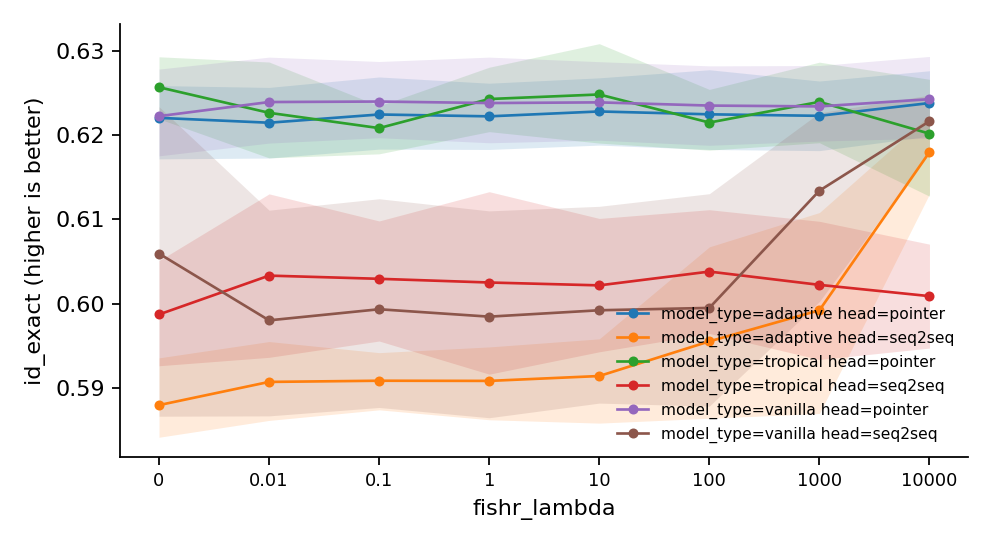
\includegraphics[width=\textwidth]{metric_id_exact.png}
\caption{\texttt{id\_exact} against \texttt{fishr\_lambda}: the mean over seeds with a 95\% bootstrap CI, one line per combination of the other factors.}
\label{fig:id_exact}
\end{figure}

{\small
\begin{longtable}{lllrlrrr}
\caption{\texttt{id\_exact} per cell: mean, 95\% bootstrap CI, SD, seeds, diverged runs.}\label{tab:summary-id_exact}\\
\toprule
\texttt{model\_type} & \texttt{head} & \texttt{fishr\_lambda} & mean & 95\% CI & SD & $n$ & div.\\
\midrule
\endhead
adaptive & pointer & 0 & 0.6221 & [0.617, 0.626] & 0.00574 & 5 & 0\\
adaptive & pointer & 0.01 & 0.6215 & [0.617, 0.626] & 0.00554 & 5 & 0\\
adaptive & pointer & 0.1 & 0.6225 & [0.618, 0.627] & 0.00546 & 5 & 0\\
adaptive & pointer & 1 & 0.6223 & [0.618, 0.626] & 0.00522 & 5 & 0\\
adaptive & pointer & 10 & 0.6228 & [0.619, 0.627] & 0.00531 & 5 & 0\\
adaptive & pointer & 100 & 0.6225 & [0.618, 0.628] & 0.00615 & 5 & 0\\
adaptive & pointer & 1000 & 0.6223 & [0.618, 0.626] & 0.00534 & 5 & 0\\
adaptive & pointer & 1e+04 & 0.6238 & [0.62, 0.628] & 0.00497 & 5 & 0\\
adaptive & seq2seq & 0 & 0.5879 & [0.584, 0.594] & 0.0064 & 5 & 0\\
adaptive & seq2seq & 0.01 & 0.5907 & [0.586, 0.595] & 0.00606 & 5 & 0\\
adaptive & seq2seq & 0.1 & 0.5908 & [0.587, 0.594] & 0.00474 & 5 & 0\\
adaptive & seq2seq & 1 & 0.5908 & [0.586, 0.595] & 0.00578 & 5 & 0\\
adaptive & seq2seq & 10 & 0.5914 & [0.586, 0.596] & 0.00664 & 5 & 0\\
adaptive & seq2seq & 100 & 0.5955 & [0.586, 0.607] & 0.0131 & 5 & 0\\
adaptive & seq2seq & 1000 & 0.5992 & [0.587, 0.611] & 0.0156 & 5 & 0\\
adaptive & seq2seq & 1e+04 & 0.618 & [0.613, 0.622] & 0.00631 & 5 & 0\\
tropical & pointer & 0 & 0.6257 & [0.622, 0.629] & 0.00488 & 5 & 0\\
tropical & pointer & 0.01 & 0.6227 & [0.617, 0.629] & 0.00744 & 5 & 0\\
tropical & pointer & 0.1 & 0.6209 & [0.618, 0.624] & 0.00372 & 5 & 0\\
tropical & pointer & 1 & 0.6243 & [0.62, 0.628] & 0.00509 & 5 & 0\\
tropical & pointer & 10 & 0.6249 & [0.619, 0.631] & 0.00774 & 5 & 0\\
tropical & pointer & 100 & 0.6215 & [0.618, 0.625] & 0.00461 & 5 & 0\\
tropical & pointer & 1000 & 0.624 & [0.619, 0.629] & 0.0064 & 5 & 0\\
tropical & pointer & 1e+04 & 0.6202 & [0.613, 0.627] & 0.00932 & 5 & 0\\
tropical & seq2seq & 0 & 0.5987 & [0.593, 0.605] & 0.00808 & 5 & 0\\
tropical & seq2seq & 0.01 & 0.6033 & [0.594, 0.613] & 0.013 & 5 & 0\\
tropical & seq2seq & 0.1 & 0.6029 & [0.596, 0.61] & 0.00935 & 5 & 0\\
tropical & seq2seq & 1 & 0.6025 & [0.592, 0.613] & 0.0143 & 5 & 0\\
tropical & seq2seq & 10 & 0.6022 & [0.594, 0.61] & 0.0102 & 5 & 0\\
tropical & seq2seq & 100 & 0.6038 & [0.596, 0.611] & 0.0097 & 5 & 0\\
tropical & seq2seq & 1000 & 0.6022 & [0.593, 0.61] & 0.00999 & 5 & 0\\
tropical & seq2seq & 1e+04 & 0.6009 & [0.595, 0.607] & 0.00787 & 5 & 0\\
vanilla & pointer & 0 & 0.6223 & [0.618, 0.628] & 0.00657 & 5 & 0\\
vanilla & pointer & 0.01 & 0.624 & [0.619, 0.629] & 0.00656 & 5 & 0\\
vanilla & pointer & 0.1 & 0.624 & [0.62, 0.629] & 0.00585 & 5 & 0\\
vanilla & pointer & 1 & 0.6238 & [0.619, 0.629] & 0.00643 & 5 & 0\\
vanilla & pointer & 10 & 0.6239 & [0.619, 0.629] & 0.00599 & 5 & 0\\
vanilla & pointer & 100 & 0.6235 & [0.619, 0.628] & 0.00629 & 5 & 0\\
vanilla & pointer & 1000 & 0.6234 & [0.619, 0.628] & 0.00573 & 5 & 0\\
vanilla & pointer & 1e+04 & 0.6243 & [0.62, 0.629] & 0.00611 & 5 & 0\\
vanilla & seq2seq & 0 & 0.6059 & [0.587, 0.623] & 0.0239 & 5 & 0\\
vanilla & seq2seq & 0.01 & 0.598 & [0.587, 0.611] & 0.0156 & 5 & 0\\
vanilla & seq2seq & 0.1 & 0.5993 & [0.588, 0.612] & 0.016 & 5 & 0\\
vanilla & seq2seq & 1 & 0.5984 & [0.586, 0.611] & 0.0161 & 5 & 0\\
vanilla & seq2seq & 10 & 0.5992 & [0.588, 0.612] & 0.0152 & 5 & 0\\
vanilla & seq2seq & 100 & 0.5995 & [0.588, 0.613] & 0.016 & 5 & 0\\
vanilla & seq2seq & 1000 & 0.6134 & [0.6, 0.623] & 0.0149 & 5 & 0\\
vanilla & seq2seq & 1e+04 & 0.6217 & [0.618, 0.625] & 0.00465 & 5 & 0\\
\bottomrule
\end{longtable}
}

{\small
\begin{longtable}{lllrrrl}
\caption{\texttt{id\_exact}: each level of \texttt{fishr\_lambda} against its control (0), within each combination of the other factors. parametric: Dunnett vs control.}\label{tab:control-id_exact}\\
\toprule
\texttt{model\_type} & \texttt{head} & \texttt{fishr\_lambda} & difference & 95\% CI & $p$ & \\
\midrule
\endhead
adaptive & pointer & 0.01 & $-5.800\times10^{-4}$ & [-0.0101, 0.00899] & 1.0000 & \\
adaptive & pointer & 0.1 & $4.000\times10^{-4}$ & [-0.00917, 0.00997] & 1.0000 & \\
adaptive & pointer & 1 & $1.800\times10^{-4}$ & [-0.00939, 0.00975] & 1.0000 & \\
adaptive & pointer & 10 & $7.600\times10^{-4}$ & [-0.00881, 0.0103] & 1.0000 & \\
adaptive & pointer & 100 & $4.200\times10^{-4}$ & [-0.00915, 0.00999] & 1.0000 & \\
adaptive & pointer & 1000 & $2.400\times10^{-4}$ & [-0.00933, 0.00981] & 1.0000 & \\
adaptive & pointer & 1e+04 & 0.00176 & [-0.00781, 0.0113] & 0.9949 & \\
adaptive & seq2seq & 0.01 & 0.00276 & [-0.0128, 0.0183] & 0.9958 & \\
adaptive & seq2seq & 0.1 & 0.0029 & [-0.0126, 0.0184] & 0.9944 & \\
adaptive & seq2seq & 1 & 0.00288 & [-0.0126, 0.0184] & 0.9946 & \\
adaptive & seq2seq & 10 & 0.00346 & [-0.0121, 0.019] & 0.9849 & \\
adaptive & seq2seq & 100 & 0.00758 & [-0.00795, 0.0231] & 0.6243 & \\
adaptive & seq2seq & 1000 & 0.01128 & [-0.00425, 0.0268] & 0.2346 & \\
adaptive & seq2seq & 1e+04 & 0.03008 & [0.0146, 0.0456] & $<10^{-4}$ & *\\
tropical & pointer & 0.01 & -0.00304 & [-0.0142, 0.00814] & 0.9580 & \\
tropical & pointer & 0.1 & -0.00486 & [-0.016, 0.00632] & 0.7286 & \\
tropical & pointer & 1 & -0.0014 & [-0.0126, 0.00978] & 0.9995 & \\
tropical & pointer & 10 & $-8.600\times10^{-4}$ & [-0.012, 0.0103] & 1.0000 & \\
tropical & pointer & 100 & -0.0042 & [-0.0154, 0.00698] & 0.8332 & \\
tropical & pointer & 1000 & -0.00174 & [-0.0129, 0.00944] & 0.9981 & \\
tropical & pointer & 1e+04 & -0.00552 & [-0.0167, 0.00566] & 0.6138 & \\
tropical & seq2seq & 0.01 & 0.00462 & [-0.0137, 0.023] & 0.9714 & \\
tropical & seq2seq & 0.1 & 0.00424 & [-0.0141, 0.0226] & 0.9817 & \\
tropical & seq2seq & 1 & 0.0038 & [-0.0146, 0.0222] & 0.9900 & \\
tropical & seq2seq & 10 & 0.00346 & [-0.0149, 0.0218] & 0.9941 & \\
tropical & seq2seq & 100 & 0.0051 & [-0.0133, 0.0235] & 0.9534 & \\
tropical & seq2seq & 1000 & 0.00352 & [-0.0148, 0.0219] & 0.9935 & \\
tropical & seq2seq & 1e+04 & 0.00218 & [-0.0162, 0.0205] & 0.9997 & \\
vanilla & pointer & 0.01 & 0.00168 & [-0.00915, 0.0125] & 0.9982 & \\
vanilla & pointer & 0.1 & 0.00174 & [-0.00909, 0.0126] & 0.9977 & \\
vanilla & pointer & 1 & 0.00156 & [-0.00927, 0.0124] & 0.9988 & \\
vanilla & pointer & 10 & 0.00164 & [-0.00919, 0.0125] & 0.9984 & \\
vanilla & pointer & 100 & 0.00126 & [-0.00957, 0.0121] & 0.9997 & \\
vanilla & pointer & 1000 & 0.00116 & [-0.00967, 0.012] & 0.9998 & \\
vanilla & pointer & 1e+04 & 0.00202 & [-0.00881, 0.0128] & 0.9945 & \\
vanilla & seq2seq & 0.01 & -0.00794 & [-0.036, 0.0201] & 0.9487 & \\
vanilla & seq2seq & 0.1 & -0.00662 & [-0.0346, 0.0214] & 0.9793 & \\
vanilla & seq2seq & 1 & -0.0075 & [-0.0355, 0.0205] & 0.9610 & \\
vanilla & seq2seq & 10 & -0.00674 & [-0.0348, 0.0213] & 0.9773 & \\
vanilla & seq2seq & 100 & -0.00646 & [-0.0345, 0.0216] & 0.9818 & \\
vanilla & seq2seq & 1000 & 0.00748 & [-0.0205, 0.0355] & 0.9615 & \\
vanilla & seq2seq & 1e+04 & 0.01574 & [-0.0123, 0.0438] & 0.4832 & \\
\bottomrule
\end{longtable}
}

{\small
\begin{longtable}{llrrrrr}
\caption{\texttt{id\_exact} against log10 \texttt{fishr\_lambda}: parametric: OLS slope t-test, seed-bootstrap CI, with the Jonckheere--Terpstra ordered-trend $\tau$ and $p$.}\label{tab:trend-id_exact}\\
\toprule
\texttt{model\_type} & \texttt{head} & estimate & 95\% CI & $p$ & JT $\tau$ & JT $p$\\
\midrule
\endhead
adaptive & pointer & $2.479\times10^{-4}$ & [$1.25\times10^{-4}$, $3.71\times10^{-4}$] & 0.5637 & 0.112 & 0.3985\\
adaptive & seq2seq & 0.003694 & [0.00282, 0.0052] & 0.0001 & 0.389 & 0.0032\\
tropical & pointer & $-1.429\times10^{-4}$ & [$-7.09\times10^{-4}$, $2.54\times10^{-4}$] & 0.7904 & 0.00762 & 0.9650\\
tropical & seq2seq & $-2.664\times10^{-4}$ & [$-8.45\times10^{-4}$, $3.24\times10^{-4}$] & 0.7543 & -0.0971 & 0.4731\\
vanilla & pointer & $-1.571\times10^{-5}$ & [$-8.86\times10^{-5}$, $4.43\times10^{-5}$] & 0.9740 & 0.0114 & 0.9416\\
vanilla & seq2seq & 0.003581 & [0.00108, 0.00609] & 0.0058 & 0.427 & 0.0018\\
\bottomrule
\end{longtable}
}

{\small
\begin{longtable}{lrrrl}
\caption{\texttt{id\_exact}: paired contrasts by seed, Holm-corrected across the cells. parametric: paired t-test by seed, Holm.}\label{tab:paired-id_exact}\\
\toprule
contrast (within) & difference & 95\% CI & $p$ & \\
\midrule
\endhead
\stackcell{model\_type: tropical - vanilla\\\footnotesize head=pointer fishr\_lambda=0 } & 0.00344 & [-0.00118, 0.00806] & 1.0000 & \\
\stackcell{model\_type: tropical - vanilla\\\footnotesize head=pointer fishr\_lambda=0.01 } & -0.00128 & [-0.0039, 0.00134] & 1.0000 & \\
\stackcell{model\_type: tropical - vanilla\\\footnotesize head=pointer fishr\_lambda=0.1 } & -0.00316 & [-0.0083, 0.00198] & 1.0000 & \\
\stackcell{model\_type: tropical - vanilla\\\footnotesize head=pointer fishr\_lambda=1 } & $4.800\times10^{-4}$ & [-0.00205, 0.00301] & 1.0000 & \\
\stackcell{model\_type: tropical - vanilla\\\footnotesize head=pointer fishr\_lambda=10 } & $9.400\times10^{-4}$ & [-0.00295, 0.00483] & 1.0000 & \\
\stackcell{model\_type: tropical - vanilla\\\footnotesize head=pointer fishr\_lambda=100 } & -0.00202 & [-0.00484, $8.04\times10^{-4}$] & 1.0000 & \\
\stackcell{model\_type: tropical - vanilla\\\footnotesize head=pointer fishr\_lambda=1000 } & $5.400\times10^{-4}$ & [-0.00122, 0.0023] & 1.0000 & \\
\stackcell{model\_type: tropical - vanilla\\\footnotesize head=pointer fishr\_lambda=1e+04 } & -0.0041 & [-0.0126, 0.0044] & 1.0000 & \\
\stackcell{model\_type: tropical - vanilla\\\footnotesize head=seq2seq fishr\_lambda=0 } & -0.00724 & [-0.0376, 0.0231] & 1.0000 & \\
\stackcell{model\_type: tropical - vanilla\\\footnotesize head=seq2seq fishr\_lambda=0.01 } & 0.00532 & [-0.0225, 0.0331] & 1.0000 & \\
\stackcell{model\_type: tropical - vanilla\\\footnotesize head=seq2seq fishr\_lambda=0.1 } & 0.00362 & [-0.0216, 0.0289] & 1.0000 & \\
\stackcell{model\_type: tropical - vanilla\\\footnotesize head=seq2seq fishr\_lambda=1 } & 0.00406 & [-0.0262, 0.0343] & 1.0000 & \\
\stackcell{model\_type: tropical - vanilla\\\footnotesize head=seq2seq fishr\_lambda=10 } & 0.00296 & [-0.0227, 0.0287] & 1.0000 & \\
\stackcell{model\_type: tropical - vanilla\\\footnotesize head=seq2seq fishr\_lambda=100 } & 0.00432 & [-0.0203, 0.029] & 1.0000 & \\
\stackcell{model\_type: tropical - vanilla\\\footnotesize head=seq2seq fishr\_lambda=1000 } & -0.0112 & [-0.0376, 0.0152] & 1.0000 & \\
\stackcell{model\_type: tropical - vanilla\\\footnotesize head=seq2seq fishr\_lambda=1e+04 } & -0.0208 & [-0.0309, -0.0107] & 0.0750 & \\
\stackcell{model\_type: adaptive - vanilla\\\footnotesize head=pointer fishr\_lambda=0 } & $-2.000\times10^{-4}$ & [-0.00598, 0.00558] & 1.0000 & \\
\stackcell{model\_type: adaptive - vanilla\\\footnotesize head=pointer fishr\_lambda=0.01 } & -0.00246 & [-0.00393, $-9.89\times10^{-4}$] & 0.1553 & \\
\stackcell{model\_type: adaptive - vanilla\\\footnotesize head=pointer fishr\_lambda=0.1 } & -0.00154 & [-0.0025, $-5.80\times10^{-4}$] & 0.1683 & \\
\stackcell{model\_type: adaptive - vanilla\\\footnotesize head=pointer fishr\_lambda=1 } & -0.00158 & [-0.00349, $3.34\times10^{-4}$] & 1.0000 & \\
\stackcell{model\_type: adaptive - vanilla\\\footnotesize head=pointer fishr\_lambda=10 } & -0.00108 & [-0.00278, $6.21\times10^{-4}$] & 1.0000 & \\
\stackcell{model\_type: adaptive - vanilla\\\footnotesize head=pointer fishr\_lambda=100 } & -0.00104 & [-0.00261, $5.32\times10^{-4}$] & 1.0000 & \\
\stackcell{model\_type: adaptive - vanilla\\\footnotesize head=pointer fishr\_lambda=1000 } & -0.00112 & [-0.00244, $2.04\times10^{-4}$] & 1.0000 & \\
\stackcell{model\_type: adaptive - vanilla\\\footnotesize head=pointer fishr\_lambda=1e+04 } & $-4.600\times10^{-4}$ & [-0.00241, 0.00149] & 1.0000 & \\
\stackcell{model\_type: adaptive - vanilla\\\footnotesize head=seq2seq fishr\_lambda=0 } & -0.01802 & [-0.0454, 0.00935] & 1.0000 & \\
\stackcell{model\_type: adaptive - vanilla\\\footnotesize head=seq2seq fishr\_lambda=0.01 } & -0.00732 & [-0.0315, 0.0168] & 1.0000 & \\
\stackcell{model\_type: adaptive - vanilla\\\footnotesize head=seq2seq fishr\_lambda=0.1 } & -0.0085 & [-0.0333, 0.0163] & 1.0000 & \\
\stackcell{model\_type: adaptive - vanilla\\\footnotesize head=seq2seq fishr\_lambda=1 } & -0.00764 & [-0.0329, 0.0176] & 1.0000 & \\
\stackcell{model\_type: adaptive - vanilla\\\footnotesize head=seq2seq fishr\_lambda=10 } & -0.00782 & [-0.0314, 0.0158] & 1.0000 & \\
\stackcell{model\_type: adaptive - vanilla\\\footnotesize head=seq2seq fishr\_lambda=100 } & -0.00398 & [-0.022, 0.0141] & 1.0000 & \\
\stackcell{model\_type: adaptive - vanilla\\\footnotesize head=seq2seq fishr\_lambda=1000 } & -0.01422 & [-0.0466, 0.0182] & 1.0000 & \\
\stackcell{model\_type: adaptive - vanilla\\\footnotesize head=seq2seq fishr\_lambda=1e+04 } & -0.00368 & [-0.0101, 0.00273] & 1.0000 & \\
\stackcell{head: pointer - seq2seq\\\footnotesize model\_type=adaptive fishr\_lambda=0 } & 0.03416 & [0.0226, 0.0457] & 0.0214 & *\\
\stackcell{head: pointer - seq2seq\\\footnotesize model\_type=adaptive fishr\_lambda=0.01 } & 0.03082 & [0.0271, 0.0346] & 0.0005 & *\\
\stackcell{head: pointer - seq2seq\\\footnotesize model\_type=adaptive fishr\_lambda=0.1 } & 0.03166 & [0.0265, 0.0368] & 0.0016 & *\\
\stackcell{head: pointer - seq2seq\\\footnotesize model\_type=adaptive fishr\_lambda=1 } & 0.03146 & [0.0286, 0.0343] & 0.0002 & *\\
\stackcell{head: pointer - seq2seq\\\footnotesize model\_type=adaptive fishr\_lambda=10 } & 0.03146 & [0.0254, 0.0376] & 0.0028 & *\\
\stackcell{head: pointer - seq2seq\\\footnotesize model\_type=adaptive fishr\_lambda=100 } & 0.027 & [0.0101, 0.0439] & 0.1486 & \\
\stackcell{head: pointer - seq2seq\\\footnotesize model\_type=adaptive fishr\_lambda=1000 } & 0.02312 & [0.00346, 0.0428] & 0.3093 & \\
\stackcell{head: pointer - seq2seq\\\footnotesize model\_type=adaptive fishr\_lambda=1e+04 } & 0.00584 & [$-6.78\times10^{-4}$, 0.0124] & 0.4227 & \\
\stackcell{head: pointer - seq2seq\\\footnotesize model\_type=tropical fishr\_lambda=0 } & 0.02702 & [0.02, 0.034] & 0.0082 & *\\
\stackcell{head: pointer - seq2seq\\\footnotesize model\_type=tropical fishr\_lambda=0.01 } & 0.01936 & [0.00605, 0.0327] & 0.1719 & \\
\stackcell{head: pointer - seq2seq\\\footnotesize model\_type=tropical fishr\_lambda=0.1 } & 0.01792 & [0.00777, 0.0281] & 0.1205 & \\
\stackcell{head: pointer - seq2seq\\\footnotesize model\_type=tropical fishr\_lambda=1 } & 0.02182 & [0.00874, 0.0349] & 0.1371 & \\
\stackcell{head: pointer - seq2seq\\\footnotesize model\_type=tropical fishr\_lambda=10 } & 0.0227 & [0.0184, 0.027] & 0.0026 & *\\
\stackcell{head: pointer - seq2seq\\\footnotesize model\_type=tropical fishr\_lambda=100 } & 0.01772 & [0.00829, 0.0272] & 0.1032 & \\
\stackcell{head: pointer - seq2seq\\\footnotesize model\_type=tropical fishr\_lambda=1000 } & 0.02176 & [0.0139, 0.0297] & 0.0268 & *\\
\stackcell{head: pointer - seq2seq\\\footnotesize model\_type=tropical fishr\_lambda=1e+04 } & 0.01932 & [0.00656, 0.0321] & 0.1640 & \\
\stackcell{head: pointer - seq2seq\\\footnotesize model\_type=vanilla fishr\_lambda=0 } & 0.01634 & [-0.0123, 0.0449] & 0.5636 & \\
\stackcell{head: pointer - seq2seq\\\footnotesize model\_type=vanilla fishr\_lambda=0.01 } & 0.02596 & [$5.62\times10^{-4}$, 0.0514] & 0.4227 & \\
\stackcell{head: pointer - seq2seq\\\footnotesize model\_type=vanilla fishr\_lambda=0.1 } & 0.0247 & [$-5.03\times10^{-4}$, 0.0499] & 0.4227 & \\
\stackcell{head: pointer - seq2seq\\\footnotesize model\_type=vanilla fishr\_lambda=1 } & 0.0254 & [$-4.21\times10^{-5}$, 0.0508] & 0.4227 & \\
\stackcell{head: pointer - seq2seq\\\footnotesize model\_type=vanilla fishr\_lambda=10 } & 0.02472 & [$1.19\times10^{-5}$, 0.0494] & 0.4227 & \\
\stackcell{head: pointer - seq2seq\\\footnotesize model\_type=vanilla fishr\_lambda=100 } & 0.02406 & [-0.00143, 0.0495] & 0.4227 & \\
\stackcell{head: pointer - seq2seq\\\footnotesize model\_type=vanilla fishr\_lambda=1000 } & 0.01002 & [-0.0111, 0.0312] & 0.5636 & \\
\stackcell{head: pointer - seq2seq\\\footnotesize model\_type=vanilla fishr\_lambda=1e+04 } & 0.00262 & [-0.00402, 0.00926] & 0.5636 & \\
\bottomrule
\end{longtable}
}


\section{Curves}
\begin{figure}[tbp]
\centering
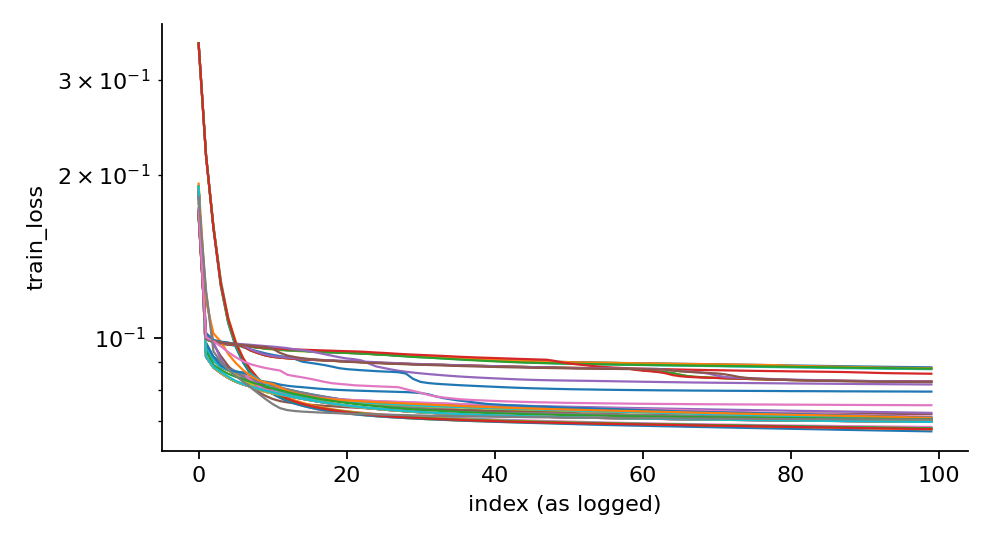
\includegraphics[width=\textwidth]{curve_train_loss.png}
\caption{\texttt{train\_loss}, the mean over seeds per cell.}
\label{fig:curve-1}
\end{figure}
\begin{figure}[tbp]
\centering
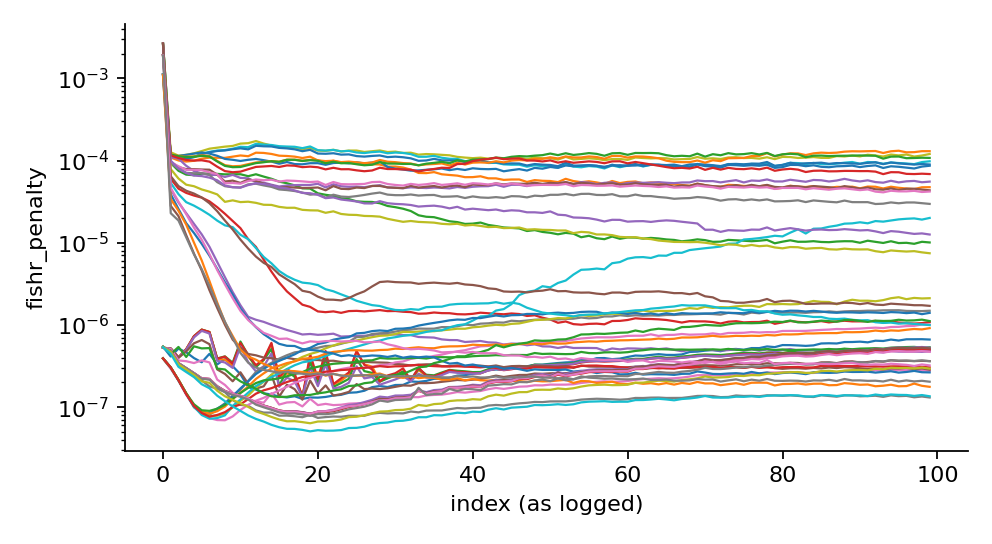
\includegraphics[width=\textwidth]{curve_fishr_penalty.png}
\caption{\texttt{fishr\_penalty}, the mean over seeds per cell.}
\label{fig:curve-2}
\end{figure}
\begin{figure}[tbp]
\centering
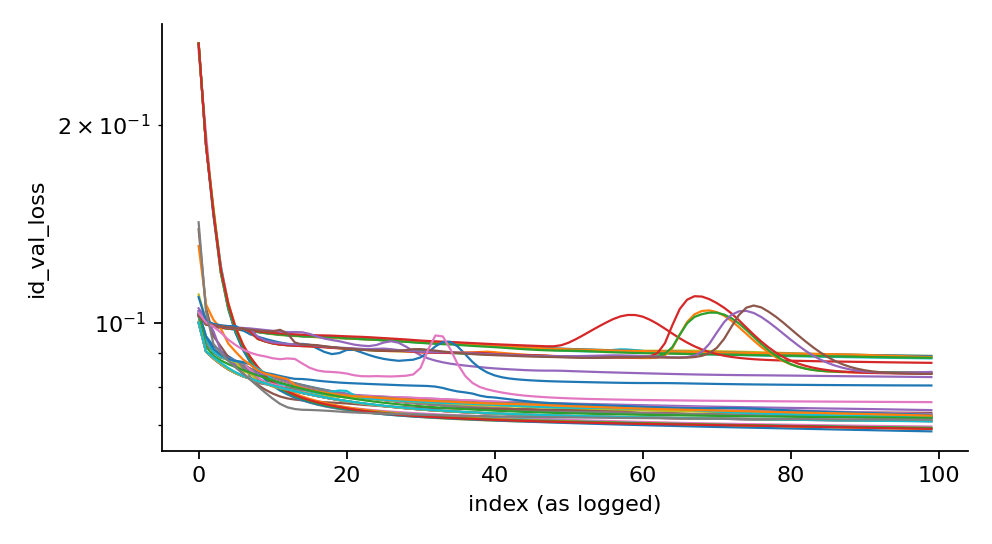
\includegraphics[width=\textwidth]{curve_id_val_loss.png}
\caption{\texttt{id\_val\_loss}, the mean over seeds per cell.}
\label{fig:curve-3}
\end{figure}

\section{Configuration}
The base configuration every run shares (frozen hash \texttt{765d817c3d73}); factor levels are in \autoref{tab:summary-ood_len_f1}.
{\footnotesize
\begin{verbatim}
task:
  name: FloydWarshallDataset
  value_range:
  - 1
  - 15
  target_range: null
  weight_range: null
  adversarial_range:
  - 10
  - 20
  noise_prob: 0.0
data:
  train_lengths:
  - 4
  - 5
  - 6
  - 7
  - 8
  ood_lengths:
  - 12
  - 16
  ood_value_range:
  - 16
  - 30
  ood_noise_range:
  - 1
  - 10
  ood_noise_prob: 0.5
  n_per_length: 20000
  n_eval_per_length: 2000
  curve_eval_limit: 256
model:
  d_model: 64
  n_heads: 2
  num_layers: 1
  dropout: 0.0
  tropical_impl: legacy
optim:
  lr: 0.0001
  epochs: 100
  batch_size: 8
  eval_batch_size: 8
fishr:
  ema: 0.95
  anneal_iters: 1500
  reset_optimizer: true
\end{verbatim}
}
Store: \texttt{campaigns/tropical/FloydWarshall/results}.
\end{document}